% 文档类(模板)
\documentclass[%
  type = bachelor,  % 本科论文(设计)
  % oneside,        % 单面模式
  twoside,          % 双面模式(openany)
]{nwafuthesis}
% 导言区

% 将需要载入的宏包统一在settings/package.tex中进行管理
% 请按自己的论文排版需求,加载需要的宏包

% TikZ绘图宏包

\makeatletter
\let\theoremstyle\relax
\let\newtheoremstyle\relax
\let\proof\relax
\let\endproof\relax
\makeatother

\usepackage{amsthm}

\usepackage{amsmath}

\usepackage{tikz}
% 卧图卧表宏包
\usepackage{lscape}
% 引号宏包
\usepackage{csquotes}
% 子图表宏包
\usepackage{subcaption}
% 双语标题宏包
\usepackage{bicaption}
% 合并表格行宏包
\usepackage{multirow}
% csv数据处理宏包
\usepackage{datatool}
% 单位符号宏包
\usepackage{siunitx}
% 跨页长表格宏包
\usepackage{longtable}
% 三线表宏包
\usepackage{booktabs}
% 新一代表格排版宏包
\usepackage{tabularray}
% 表格注释说明宏包
\usepackage{threeparttable}
% 带边框小页环境
\usepackage{boxedminipage2e}

\usepackage{empheq}

\usepackage{csvsimple}

\usepackage{caption}

\usepackage{tabularx}

\usepackage{float}

\usepackage{algorithm}
\usepackage{algorithmicx}

\makeatletter
\newenvironment{breakablealgorithm}
{%\begin{breakablealgorithm}
	\begin{center}
		\refstepcounter{algorithm}% New algorithm
		\hrule height.8pt depth0pt \kern2pt% \@fs@pre for \@fs@ruled
		\renewcommand{\caption}[2][\relax]{% Make a new \caption
			{\raggedright\textbf{\ALG 算法~\thealgorithm} ##2\par}%
			\ifx\relax##1\relax % #1 is \relax
			\addcontentsline{loa}{algorithm}{\protect\numberline{\thealgorithm}##2}%
			\else % #1 is not \relax
			\addcontentsline{loa}{algorithm}{\protect\numberline{\thealgorithm}##1}%
			\fi
			\kern2pt\hrule\kern2pt
		}
	}{%\end{breakablealgorithm}
		\kern2pt\hrule\relax% \@fs@post for \@fs@ruled
	\end{center}
}\makeatother
\usepackage[noend]{algpseudocode}

%%% Local Variables:
%%% mode: latex
%%% TeX-master: "../main.tex"
%%% End:

% 将必要的设置统一在settings/format.tex中进行管理
% ==============LaTeX命令排版命令(排版示例文档时使用)========================
\newcommand\cs[1]{\texttt{\textbackslash#1}}
\newcommand\pkg[1]{\texttt{#1}\textsuperscript{PKG}}
\newcommand\env[1]{\texttt{#1}}
\newcommand{\note}[1]{{%
  \color{magenta}{\bfseries 注意:}\emph{#1}}}
%% ==================================================

% 设置插图目录
\graphicspath{{./figs/},{./logo/}}
%% ==================================================

% 引入tabularray的booktabs库
\UseTblrLibrary{booktabs}

%% 自定义相关的名称宏命令
%% ==================================================
% 西北农林科技大学各单位名称
\newcommand{\nwsuaf}{西北农林科技大学}
\newcommand{\cie}{信息工程学院}
\newcommand{\ca}{农学院}
\newcommand{\cpp}{植物保护学院}
\newcommand{\chc}{园艺学院}
\newcommand{\cast}{动物科技学院}
\newcommand{\cvm}{动物医学院}
\newcommand{\cf}{林学院}
\newcommand{\claa}{风景园林艺术学院}
\newcommand{\cnre}{资源环境学院}
\newcommand{\cwrae}{水利与建筑工程学院}
\newcommand{\cmee}{机械与电子工程学院}
\newcommand{\cfse}{食品科学与工程学院}
\newcommand{\celg}{葡萄酒学院}
\newcommand{\clsc}{生命科学学院}
\newcommand{\cst}{理学院}
\newcommand{\ccp}{化学与药学院}
\newcommand{\cem}{经济管理学院}
\newcommand{\cm}{马克思主义学院}
\newcommand{\chsd}{人文社会发展学院}
\newcommand{\dfl}{外语系}
\newcommand{\iec}{创新实验学院}
\newcommand{\ci}{国际学院}
\newcommand{\dpe}{体育部}
\newcommand{\cvae}{成人教育}
\newcommand{\iswc}{水土保持研究所}

%%% Local Variables:
%%% mode: latex
%%% TeX-master: "../main.tex"
%%% End:


% 编写测试文档用到的两个宏包,若不需要,可能删除
% 中文乱数假文宏包
\usepackage{zhlipsum}
% 最小工作示例(MWE)宏包,主要用于插图示例
\usepackage{mwe}

% 排版设置
\nwafuset{
% 论文格式
  style = {
    % font          = times*,           % 选择英文字体(需要安装有该字体,建议自动配置)
    % cjk-font      = adobe,            % 选择中文字体(需要安装有该字体,建议自动配置)
    hyperlink     = color,            % 超链接颜色
    % withchapter = false,            % 章标题是否为章模式(仅本科生需要)
    bib-resource  = {bib/sample.bib}, % 参考文献数据源文件名,注意需要完整路径及后缀名
  },
% 信息录入
  info = {
    grade = {2023}, % 毕业年份(届)
    enroll = {2019}, % 入学年份(级)
    class-id = {1}, % 班级号
    btype = {paper}, % 本科类型(论文/设计)
    % btype = {design},
    title = { 基于粗糙集方法的粮食安全分析 }, % 中文题目
    title* = { Food Security Analysis Based on Rough Set Method }, % 英文题目
    department = { 理学院 }, % 学院名称
    major = {信息与计算科学}, % 专业
    author = { 于恒彬 }, % 作者中文名称
    supervisor = { 杨斌 }, % 指导教师
    cosupervisor = {无}, % 协助指导教师
    date = {\datezh}, % 论文提交时间
    student-id = {2019013914}, % 学号
  },
}
% 录入摘要
\nwafuset{
  abstract = {
    abstractfile  = { contents/chap00-abs-zh.tex }, % 中文摘要文件名称,注意需要有.tex后缀名
    abstractfile* = { contents/chap00-abs-en.tex }, % 英文摘要文件名称,注意需要有.tex后缀名
    keywords      = {粮食安全,玉米生产,粗糙集,特征选择,产量预测}, % 中文关键字列表,注意用英文逗号分隔。
    keywords*     = {food security,maize production,rough set,feature selection,yield prediction}, % 英文关键字列表,注意用英文逗号分隔
  },
}
% 正文区(有且只能有一个)
\begin{document}
% 这个命令用来关闭版心底部强制对齐,
% 可以减少不必要的 underfull \vbox 提示,但会影响排版效果
% \raggedbottom

% 由于论文模板中已设计了自动排版封面、摘要、目录等功能,
% 因此,无需手动排版。

% 主体部分是论文的核心
\mainmatter

% 建议采用多文件编译的方式编写论文,
% 比较好的做法是把每一章放进一个单独的 tex 文件里,
% 并在这里用 \include 导入,如:
% 本文件是示例论文的一部分
% 论文的主文件是位于上级目录的 `main.tex`

\chapter{引言}
本章主要介绍粗糙集方法及我国粮食安全现状,粗糙集方法分析粮食安全的目的及意义。

\section{研究背景}
俄乌冲突作为2022年世界经济形势发展的最大影响因素,对全球各国经济发展、能源供应、资源贸易等方面都造成了较为严重的冲击,其中对全球粮食等农产品产业链产生了重要影响。

俄罗斯与乌克兰作为国际上重要的粮食生产与出口大国,在全球粮食产业链中具有着重要的地位。在冲突爆发前的2021年中,两国大麦、小麦和玉米的合计产量占据全球总量的19\%、14.3\%和4.6\%,且全球32.5\%的大麦、30.6\%的小麦及19.7\%的玉米出口均来自俄乌两国\cite{俄乌冲突的蝴蝶效应与中国粮食安全的地缘风险}。又因为俄乌两国自身在粮食消费方面的数量有限,其粮食出口量在全球中占据的份额远大于产量所占据的份额,因此两国在全球的粮食贸易中占有重要的地位。同时,俄乌两国作为全球的粮食出口大国,其粮食主要出口至北非、中东、南亚地区的低收入缺粮国,在维持这些国家的粮食供给方面起着重要作用。根据联合国粮食及农业组织数据库的统计显示,一些非洲、亚洲等地一些最不发达国家或低收入国家对俄乌粮食有着很强的依赖度,俄乌两国的粮食出口变化将会对很多国家造成较为严重的影响\cite{乌克兰危机对全球粮食安全的影响与中国应对策略}。此外,俄乌不仅是主要的粮食生产与出口国,还是农作物肥料的主要供应国,两国在全球化肥出口贸易上占据全球总额的近四分之一,是全球化肥供应的主要力量\cite{俄乌冲突对全球和我国粮食安全短期影响及建议}。

俄乌冲突导致了全球农业产业链受到了严重的冲击,其造成了交战地区的粮食生产中断,粮食贸易、化肥和能源等资源的供应也几乎中断,同时北约对俄罗斯的经济制裁以及由此引发的反制裁措施严重破坏了区域经济秩序,进一步全面推高了农业生产成本。此外,粮食、化肥和能源的供应短缺预期也加剧了市场的恐慌,引发了农产品价格的普涨,严重影响了全球部分进口消费区域的粮食安全\cite{俄乌冲突对中国粮食安全的影响}。

俄乌冲突造成的全球粮食安全危机对我国有着一定的影响\cite{俄乌冲突对中国农产品供需直接影响分析,俄乌冲突对中国粮食安全的影响}。目前我国粮食安全总体形势良好,国内粮食供应充足,价格基本稳定,生产能够保障有序开展。从短期来看,对我国有着农产品价格有着一定的冲击,从长期来看,也为我国也为我国敲响了粮食安全的警钟,再次提醒我们落实粮食安全战略的艰巨性和复杂性。其中,乌克兰是全球第四大玉米出口国,2020年占全球玉米出口量的14.85\%,我国自乌克兰进口的玉米量占其出口总量的28.31\%。同时2021年我国自乌克兰进口的玉米量约占我国总玉米进口量的30\%,此次冲突对我国玉米供应将造成一定的影响,或部分推升国内玉米价格。而我国大麦进口主要用途为饲料用粮,作为玉米的主要替代品,乌克兰是中国大麦的主要供应国,乌克兰大麦占中国进口量的26\%,因此或也将部分推升国内大麦价格。我国小麦自给率高,国家小麦储备充足,市场稳定性较强,俄乌冲突对小麦影响有限。此外,我国化肥产业自给率较高,但国际化肥市场的价格飞涨,一定程度上会提高农民的农业生产成本。这对于我国外贸依存度最大的大豆以及相关饲料产业和养殖业有一定影响\cite{俄乌冲突对我国粮食安全的影响及其对策研究}。
\section{研究现状}

\subsection{粗糙集}
粗糙集的概念最初由Pawlak\cite{pawlak1995rough}提出,作为一种处理数据分析中的不精确、模糊和不确定性的数学方法。这一理论已被充分证明在成功解决各种问题方面具有实用性和通用性\cite{1998Rough,huang1992intelligent,ziarko1994rough}。粗糙集理论的一个重要应用是数据库中的属性约简。给定一个具有离散化属性值的数据集,可以找到原始属性的子集,该子集包含与原始属性相同的信息。区别于其他理论而言,属性约简的概念可以被视为粗糙集理论中最有力、最重要的结果。属性约简的粗糙集方法可以作为一种纯粹的结构方法,使用数据集中包含的信息降维并保留特征的含义\cite{tsang2008attributes}。

其中,基于属性重要度的属性约简算法作为粗糙集属性约简算法的一个分支,在计算属性重要度与属性约简方面有着较大的潜力。路松峰等人\cite{路松峰2008}对属性依赖没有考虑条件属性间的依赖关系的问题,提出了ARA属性约简算法;翟俊海等人\cite{翟俊海2014}针对属性依赖度的计算忽略了边界概率分布信息这一问题,提出了利用最小相关性和最大依赖度准则求决策表属性约简的改进算法。廖倩\cite{基于粗糙集和模糊粗糙集的属性约简研究}针对现有的基于正域的属性约简算法的弊端,提出了新的属性重要度计算方法,并针对模糊粗糙集属性约简算法中属性组合爆炸问题提出改进属性约简算法,有效减少了计算量。此外,还有其他研究着眼于属性重要度的度量与定义,针对不同问题提出了不同的算法。

然而,如\cite{jensen2004fuzzy}中所述,属性的值可以是符号值和实值。传统的粗糙集理论在处理此类实值属性时会遇到困难。解决这个问题的一种方法是预先离散属性值\cite{1998Discretization,},并创建一个新的具有符号属性值的数据集。然而,使用这种方法会造成信息丢失。另一种方法是使用模糊粗糙集。模糊粗糙集包含了模糊性和不可分辨性这两个相关但不同的概念,这两个概念都是由于知识中存在的不确定性而产生的。在模糊粗糙集中,模糊相似关系被用来表征两个对象之间的相似程度,而不是在清晰粗糙集中使用的等价关系。如果相似度为1,那么它们是不可分辨的。如果相似度为0,则它们是可辨别的。如果相似度取0到1之间的值,那么这两个对象在一定程度上相似。然而,不同的模糊相似性关系可能产生不同程度的相似性,因此信息丢失也是可能的。不合理的模糊相似关系会带来较大的信息损失。这个问题可以通过定义一个合理的模糊相似关系来解决。

模糊粗糙集(以下简记FRS)由Dubois和Prade\cite{dubois1990rough}于1990年提出,是一种将模糊集与粗糙集理论相结合的模型。模糊粗糙集理论在处理不确定性、不准确数据和不完整数据方面发挥着关键作用。1992年,Kuncheva\cite{KUNCHEVA1992147}首次提出了一种使用模糊粗糙集的特征选择方法。其利用弱模糊划分方法定义了模糊的正、负和边界区域,提出了特征选择的思想。然而,由于FRS在当时刚刚诞生,它们并没有引起足够的关注。2004年,Jensen等人\cite{2004Fuzzy}提出了一种基于FRS的属性约简方法。从那时起,基于FRS的属性约简受到了广泛的关注。根据所使用的不同约简规则,基于FRS的属性约简方法可以大致可分为三类:基于模糊依赖性的、基于模糊不确定性测度的以及基于模糊辨别矩阵的。

在此,重点介绍基于模糊依赖度的模糊粗糙集属性约简方法。2005年,由于\cite{2004Fuzzy}中提出的方法无法经常找到最优子集,Jenshen和Shen\cite{2005Fuzzy}提出了一种基于蚁群优化的特征选择策略来解决这个问题。然后将该方法应用于FRS下的最优特征子集的求解问题。针对\cite{2004Fuzzy}中算法的不收敛问题,在通过实验发现该问题后,Bhatt等人\cite{2005On,2005compact}提出了一种在域附近的改进策略,以提高算法的性能。考虑到在许多情况下可分辨性的概念更为自然有效,Cornelis等人\cite{2010Feature}提出了使用基于模糊容差关系的经典粗糙集框架的推广,然后引入了基于正域的模糊决策约简的概念。2010年,Hu等人\cite{2010Gaussian}将高斯核与FRS相结合,提出了一种基于高斯核的FRS模型,并基于所提出的模型设计了一种基于高斯核的特征选择算法。2013年,Mac ParthaláIn等人\cite{mac2013unsupervised}提出了一种基于模糊依赖性的无监督特征方法。在后续的研究中,大多数针对FRS方法耗时难以忍受的问题进行了加速研究,Qian等人\cite{qian2015fuzzy}提出了一种用于特征选择的加速器方法,Zhang等人\cite{zhang2018fuzzy}针对FRS代表实例的特征选择问题提出了一种基于代表实例的特性选择方法,Ni等人\cite{ni2019positive}基于Dubois和Prade的模糊粗糙模型,设计了一种基于正区域的加速器算法。这些研究都将模糊粗糙集方法推向了分析大规模和高维数据集的应用。

% 然而,FRS方法的时间消耗对于分析大规模和高维数据集来说是非常难以忍受的,在此之前虽然已经开发了许多基于启发式模糊粗糙集的特征选择算法,但这些方法通常在计算上仍然很耗时。2015年,为了进一步解决这个问题,Qian等人提出了一种用于特征选择的加速器方法[42]。他们选择了Hu等人[68]提出的模糊粗糙模型。Zhang等人在2018年研究了基于FRS的代表实例的特征选择问题,并提出了一种基于代表实例的特性选择方法[76]。2019年,Ni等人基于Dubois和Prade的模糊粗糙模型,设计了一种基于正区域的加速器算法[81]。此外,在模糊正区域和关键实例集的增量机制的基础上,他们提出了一种基于FRS的增量特征选择算法[82]。在上述基于依赖性的特征选择方法中,大多数方法都采用模糊关系的交集(连接)运算来构造属性约简的隶属度函数。采用不同的模糊上下近似算子也会有着不同的特征选择效果,针对不同类型的数据,在应用中需要根据数据结构选择合适的属性约简算法。

同时,模糊粗糙集已经在许多领域得到了应用。Xie等人\cite{xie2017evaluation}将模糊粗糙集应用于变压器油纸绝缘状态评估,为变压器油纸的绝缘状态评估提供了新的思路,在工程应用中具有实用价值。Zhang等人\cite{ZHANGChao1531}将模糊粗糙集应用于职业评估等多属性决策问题,并利用模糊集和粗糙集在不确定决策中的优势,为决策者提供有价值的决策模型。Guo等人\cite{rongchao2017fuzzy}在多标签分类任务中使用了模糊粗糙集模型,通过特征选择得到分类效果良好。曹愈远等人\cite{曹愈远2017基于模糊粗糙集}将模糊粗糙集与支持向量机相结合,用于航空发动机故障诊断,得到该方法具有较强的诊断能力,在不影响诊断率的情况下大大缩短了计算时间。总之,模糊粗糙集在数据挖掘中的应用是广泛的,尤其是在处理不确定、不完全和模糊信息问题时\cite{duan2020energy}。因此,本文考虑将模糊粗糙集应用到粮食安全影响因素的分析及预测中。

\subsection{粮食安全}

近年来,有部分研究着眼于利用经典变量选择方法对粮食安全进行分析。2015年,李岩岩等人\cite{基于SIR方法分析重庆市粮食产量}利用切片逆回归(SIR)方法对1978-2013年重庆市粮食总产量数据进行降维得到主要影响因素,再根据降维后的数据进行最小二乘拟合,得到了较好的预测效果。2016年,Jeong等人\cite{jeong2016random}评估了随机森林(RF)与多元线性回归(MLR)在预测小麦、玉米和土豆在全球和区域尺度上对气候和生物物理变量的作物产量反应,得到RF具有很高的预测作物产量的能力,并且在所有比较的性能统计中都优于MLR基准。2017年,马云倩等人\cite{孙君茂2018}利用Lasso方法筛选出影响我国粮食总产量的6个显著影响因素,将这6个因素作为输入因子构建粮食产量预测模型GM(1,6)进行预测,同时与原模型进行比较,预测出未来3年内我国粮食产量处于稳步增长的状态。2019年,Khaki等人\cite{khaki2019crop}设计了一种深度神经网络(DNN)方法,利用玉米杂交种的基因型和产量表现预测2017年的产量,并基于训练的DNN模型进行了特征选择,成功地降低输入空间的维数的同时又保证了预测精度没有显著下降,结果显示该模型显著优于Lasso、浅层神经网络和回归树等其他流行的方法。2022年,钟奇\cite{基于主成分分析的BP神经网络粮食产量预测模型}采用主成分分析法与BP神经网络相结合的预测模型,先利用主成分分析法对高维数据进行降维,再利用BP神经网络进行预测,得到了影响粮食生产的2个主要因素。

粗糙集方法在变量选择方面相较于传统方法有着很好的优势,仅有少数研究将粗糙集理论与粮食安全的分析结合起来。 2005年,Zhang与He\cite{2005Study}提出的基于粗糙集的灰色关联BP神经网络综合了粗糙集和灰色系统的理论,先利用灰色关联与粗糙集理论对1990-2002年我国粮食产量数据的条件属性进行约简得到关键因子,然后利用关键因子对BP神经网络进行训练和预测,大大提高了相比于一般神经网络的预测精度。2008年,韩万渠等人\cite{韩万渠2008基于粗糙集理论的我国粮食生产能力制约因素分析}基于粗糙集理论对我国粮食生产能力制约因素进行了分析,得到科研、化肥、机械是提高粮食产量的3个最重要的因素。2013年,欧阳浩等人\cite{基于粗糙集方法的广东省粮食产量影响因素分析}利用粗糙集方法对广东省粮食产量影响因素分析,得到了化肥用量、水库总容量、人均经营耕地面积三个关键影响因子。2015年,王丹丹等人\cite{基于粗糙集理论的河南省粮食产量预测研究}利用运用粗糙集理论对河南省粮食产量决策表进行属性约简。结果表明,粮食作物播种面积、化肥施用折纯量和农用机械总动力是河南省粮食产量的主要影响因素,且相对于粮食产量的重要性程度依次降低。

\section{研究的意义及创新点}
虽然我国粮食安全总体形势良好,但玉米、大豆、大麦等粮食进口需求相比较大的农产品价格仍然受到了俄乌冲突的影响。在俄乌冲突造成的粮食市场供应短缺下,很多国家将提高粮食作物的生产能力作为重要目标,扩大粮食作物的播种面积,这为我国敲响了粮食安全的警钟。

粮食安全的基石是确保粮食充足供给,粮食生产作为粮食安全中重要的一环,确保主粮作物的充足供应是粮食安全战略的关键。在当今地缘冲突影响全球粮食贸易的背景下,对我国影响较大的农产品的粮食生产将更值得我们重视。

粮食生产作为农业生产系统的一部分,其产量会受到主观客观等多种因素的影响,因此研究影响粮食生产的主要影响因素将对俄乌冲突背景下确保主粮作物的充足供应和产业调整具有重要意义。同时,为了保障粮食的安全,需要预知未来一段时间内粮食产量的变化情况,研究粮食产量的预测也是非常必要的。

基于粗糙集理论的方法与统计方法处理不确定问题完全不同,它不采用概率方法描述数据的不确定性,与这一领域传统的模糊集合论处理不精确数据的方法也不同。粗糙集方法能够分析隐藏在数据中的信息,而不需要关于数据的任何附加信息。该方法可以在保持属性集分类能力不变的情况下,进行属性约简,尽量删除冗余属性,留下对分类最重要的属性。

近5年来,绝大多数研究都倾向于利用机器学习模型来分析和预测粮食安全,近十年内很少能找到有利用粗糙集理论对粮食安全进行分析的研究,粗糙集理论的优势在于可以在尽量不损失属性集信息的条件下对数据进行降维约简,模糊粗糙集更是可以克服粗糙集方法对于离散化数据要求的局限性,而机器学习方法的一大难度在于训练过程的优化难题,将二者的优势加以结合的研究便显得尤为重要。

因此,本文选择我国受到俄乌冲突影响较严重代表性农作物-玉米作为研究对象,通过采用粗糙集方法分析影响其产量的主要因素,同时与传统特征选择方法进行比较,再利用预测模型对特征选择结果进行评价,进而得到粗糙集方法在特征选择方面相对于一般方法的优劣,最后根据特征选择结果对我国玉米生产及粮食安全提供建议。
\section{本文组织结构}
\begin{itemize}
    \item \ 第2章主要介绍基于粗糙集的属性约简,包括粗糙集的理论知识及属性约简算法。
    \item \ 第3章主要建立了基于粗糙集方法的粮食生产模型,介绍了研究数据、模型框架及模型方法。
    \item \ 第4章分别用三种特征选择方法对数据集进行处理,选出了每个特征选择方法下影响玉米生产因素最重要的前10个变量,同时得到了相应的约简数据集,并比较了三种不同算法的特征选择耗时。
    \item \ 第5章主要对第三章中的特征选择结果进行了数值实验验证。通过将不同方法下的约简数据集放入随机森林预测模型中进行训练与预测,比较每个省份的不同约简数据集在训练耗时、均方误差及预测精度上的差异,进而评价不同特征选择方法的特征选择效果。
    \item \ 第6章主要进行了粮食安全结果分析,通过对模糊粗糙集属性约简算法得到的各省影响玉米产量最重要的因素进行结果可视化,分别从化肥投入情况、成本投入情况、排灌建设情况及机械化建设情况四个方面对影响玉米产量的影响因素进行分析,对我国玉米生产及粮食安全提供了建议。
    \item \ 第7章主要总结了本文的工作,并对进一步的研究进行了展望。
\end{itemize}

\chapter{基于粗糙集的属性约简}
\label{chapter:0105}
\section{基本概念}
\label{section:粗糙集基本概念}
\subsection{粗糙集}
\newtheorem{Definition}{\hspace{2em}定义}[chapter]
\begin{Definition}[决策表]\cite{2009New}
设$I=(U,AT,V,f)$是一个信息系统, 其中$U=\{x_1,\cdots,x_n\}$为有限对象的非空集合(即论域), $AT$为属性的非空有限集合, 其中$AT=C\bigcup \{d\}$, 子集$C$和$\{d\}$分别被称为条件属性集和决策属性集. $f:U \times  AT \rightarrow V$是一个信息函数, 它将每个对象的每个属性映射为一个信息值, 其中$V=\bigcup_{a \in AT} V_{a}$是属性值的集合,$V_{a}$是属性a的值域. 这样的信息系统成为决策表, 一般简记为$I=(U,AT)$.
\end{Definition}
\begin{Definition}[划分与等价类]\cite{gu2014knowledge}
对于任意非空属性子集$P \subseteq AT$, 定义由$P$确定的U上的不可分辨关系为:
$$\operatorname{IND}(P)=\{(x, y) \in U \times U: a(x)=a(y), \forall a \in P\}.$$
其中, $a(x)$和$a(y)$分别为对象$x$与$y$在属性$a$上的取值.

显然, $\operatorname{IND}(P)$满足自反性, 对称性与传递性, 是$U$上的等价关系。并定义由$\operatorname{IND}(P)$生成的关于$U$的划分$U/\operatorname{IND}(P)$(简记为$U/P$)为:
$$U/\operatorname{IND}(P)=U/P=\left\{[x]_{P}: x \in U\right\}.$$
其中$[x]_{P}$表示由$x$确定的关于$P$的等价类, 即$[x]_{P}=\left\{y \in U:(x, y) \in R_{P}\right\}.$它将$U$划分为$U$上不相交子集$U/\operatorname{IND}(P)$的族.
\end{Definition}
% \begin{Definition}[等价关系与等价类]
% 对于属性集$A$的任意条件属性子集$P \subseteq A$, 定义$P$上的等价关系(也称不可分辨关系)$\operatorname{IND}(P)$为:
% $$\operatorname{IND}(P)=\{(x,y) \in U \times U | \forall a \in P, a(x)=a(y)\}$$.
% 其中, $a(x)$和$a(y)$分别为对象$x$与$y$在属性$a$上的取值.
% 如果$(x,y) \in \operatorname{IND}(P)$,则称$x$和$y$不可由$P$中的属性分辨, $P$的不可分辨关系的等价类表示为$[x]_P$.
% \end{Definition}
% \begin{Definition}[划分]
% 设$\operatorname{IND}(P)$为$P$上的等价关系, 定义由$\operatorname{IND}(P)$生成的关于$U$的划分$U/\operatorname{IND}(P)$(简记为$U/P$)为:
% $$U / \operatorname{IND}(P)=\otimes\{U / \operatorname{IND}(\{a\}) \mid a \in P\}$$.
% 其中,对于集合$A$与$B$, $\otimes$定义为:
% $$A \otimes B=\{X \cap Y \mid X \in A, Y \in B, X \cap Y \neq \emptyset\}$$.
% \end{Definition}

\begin{Definition}[粗糙集]\cite{2009New}
设有决策表$I=(U,AT)$, $X\subseteq U$是论域$U$上的一个对象子集, $P \subseteq AT$是$AT$上的条件属性子集,可以定义$X$在属性子集$P$上的$P$-下近似$\underline{P}(X)$和$P$-上近似$\overline{P}(X)$:
$$\underline{P}(X)=\left\{x \in U \mid[x]_{P} \subseteq X\right\},$$
$$\overline{P}(X)=\left\{x \in U \mid[x]_{P} \cap X \neq \emptyset \right\}.$$
元组$\langle\underline{P}(X), \overline{P} (X)\rangle$被称为$X$关于$P$的粗糙集.
\end{Definition}

对此,根据粗糙集的定义,可以引出粗糙集上对于条件属性子集$P$上正域、负域及边界域的概念.
\begin{Definition}[正域、负域、边界域]\cite{2009New}
设$X\subseteq U$是论域$U$上的一个对象子集, $P \subseteq AT$是$AT$上的条件属性子集, 决策属性集$\{d\}$划分论域$U$为$U/\{d\}$, 定义对象子集$X$在条件属性子集$P$上的正域$\operatorname{POS}_{P}(\{d\})$、负域$\operatorname{NEG}_{P}(\{d\})$及边界域$\operatorname{BND}(X)$为:
$$\operatorname{POS}_{P}(\{d\})=\bigcup_{X \in U / \{d\}} \underline{P} (X).$$
$$\operatorname{NEG}_{P}(\{d\})=U-\bigcup_{X \in U / \{d\}} \overline{P} (X).$$
$$\operatorname{BND}(X)=\overline{P}(X)-\underline{P} (X).$$
\end{Definition}
% \begin{Definition}[正域]
% 设决策属性集$\{d\}$划分论域$U$为$U/\{d\}$, 则条件属性子集$P$关于决策属性集$\{d\}$的正域定义为:
% $$\operatorname{POS}_{P}(\{d\})=\bigcup_{X \in U / \{d\}} \underline{P} (X).$$
% \end{Definition}
% \begin{Definition}[负域]
% 设决策属性集$\{d\}$划分论域$U$为$U/\{d\}$, 定义条件属性子集$P$关于决策属性集$\{d\}$的负域$\operatorname{NEG}_{P}(\{d\})$为:
% $$\operatorname{NEG}_{P}(\{d\})=U-\bigcup_{X \in U / \{d\}} \overline{P} (X).$$
% \end{Definition}
其中,正域$\operatorname{POS}_{P}(\{d\})$包含$U$的所有可以被属性$P$中的信息分类为$U/\{d\}$类的对象, 负域$\operatorname{NEG}_{P}(\{d\})$是一组不能分类为$U/\{d\}$类的对象, 边界域$\operatorname{BND}(X)$是可以但不一定可以以这种方式分类的对象的集合.
\begin{Definition}[属性的必要性]\cite{翟俊海2014}
    给定属性集$AT$的子集$P$, 对于属性子集$P$中的任意属性$a \in P$, 如果成立$\operatorname{POS}_{P}(\{d\})  =  \operatorname{POS}_{P-\{a\}}(\{d\})$, 则称属性$a$对属性子集$P$是不必要的; 否则称属性$a$对属性子集$P$是必要的. 如果属性子集$P$中的任意属性都是必要的, 则称$P$是独立的. 
\end{Definition}
\begin{Definition}[约简决策表]\cite{翟俊海2014}
    设决策表$I=(U,AT)$对于给定的属性子集$P \subseteq AT$, 如果$P$满足:
    $$(1)P\text{是独立的}; \qquad(2)P\text{保持正域不变,即:}\operatorname{POS}_{P}(\{d\})=\operatorname{POS}_{AT}(\{d\}).$$
    则称$P$是决策表$I$的约简; 记决策表$I$的所有约简的集合为$\operatorname{RED}_{\{d\}}(AT)$.
\end{Definition}
\begin{Definition}[依赖度]\cite{翟俊海2014}
    给定属性集$AT$中的任意条件属性$a \in AT$, 定义决策属性集$\{d\}$依赖于条件属性$a$的依赖度为$\gamma_a(\{d\})$:
    $$k=\gamma_a(\{d\})=\frac{|\operatorname{POS}_{a}(\{d\})|}{|U|}.$$
    其中$\mid * \mid$表示$*$的基数. 当$k=1$时, 表示$\{d\}$完全依赖于$a$; 当$0 < k < 1$时, 表示$\{d\}$部分依赖于$a$; 当$k=0$时, 表示$\{d\}$不依赖于$a$. 
\end{Definition}
\subsection{模糊粗糙集}
\begin{Definition}[模糊集]\cite{粒计算基础教程}
设$U$是论域, $A:U\rightarrow [0,1]$, 则称$A$是$U$上的一个模糊集, $A(x)$称为模糊集A的隶属函数. 对$\forall x \in U $,$A(x)$表示$x$隶属于模糊集$A$的程度, 简称为隶属度. $U$上全体模糊集的类称为$U$的模糊幂集, 用$F(U)$表示, $A\in F(U)$表示$A$为$U$上的一个模糊集.
\end{Definition}
\begin{Definition}[模糊集的运算]\cite{粒计算基础教程}
  设$A,B\in F(U)$, 分别称运算$A\cup B,A\cap B$为$A$与$B$的并集与交集, $A^C$称为$A$的补集, 其隶属函数分别定义为:
    $$(A \cup B)(u)=A(u) \vee B(u)=\max \{A(u), B(u)\},$$
    $$(A \cap B)(u)=A(u) \wedge B(u)=\min \{A(u), B(u)\},$$
    $$A^{C}(u)=1-A(u), \quad \forall u \in U .$$
  \end{Definition}
\begin{Definition}[模糊等价关系]\cite{粒计算基础教程}
设$U$是论域, $R \in F(U \times U)$称为$U \times U$上的一个模糊关系. 如果$R$满足:
\end{Definition}
\begin{enumerate}
\item 自反性: $R(x,x)=1, \forall x \in U$;
\item 对称性: $R(x,y)=R(y,x),\forall x,y \in U$;
\item 传递性: 对$\forall x,y,z\in U$, 有$R(x,z)\geq R(x,y)\wedge R(y,z)$.
\end{enumerate}
则称$R$是$U$上的一个模糊等价关系.

若$R$是具有自反性、对称性的模糊关系,则称 $R$ 是$U$上的模糊相似关系。

通过将模糊集的概念引入到粗糙集中,可以扩展粗糙集理论中的下近似和上近似,进而可以得到模糊粗糙集的概念。
\begin{Definition}[广义模糊粗糙集]\cite{dong2023incremental}
    设$X\in F(U)$是一个模糊集, $R$是$U$的模糊等价关系, 定义$X$基于$R$的下近似算子和上近似算子为:
$$\underline{R} X(x)=\inf _{u \in U} \max \{1-R(x, u), X(u)\},$$
$$ \overline{R} X(x)=\sup _{u \in U} \min \{R(x, u), X(u)\} .$$
其中$\underline{R}X(x)$ 是$x$一定属于$X$的程度, $\overline{R}X(x)$是$x$可能属于$X$的程度.  

$\langle\overline{R} X(x), \underline{R}X(x)\rangle$被称为模糊粗糙集$X$.
\end{Definition}
然而,现实生活中很多模糊概念很难用等价关系表示,模糊相似关系相较于模糊等价关系没有了传递性的要求,因而有着更广泛的应用背景。下面给出基于模糊相似关系定义的模糊粗糙集。

设论域$U=\{x_1,x_2,\cdots,x_n\}$为有$n$个对象的论域空间. $P=\{P_1,P_2,\cdots,P_p\}$是一组模糊条件属性, 每个属性表示为若干模糊语言项的集合$A(P_i)=\{F_{ik}:k=1,2,\cdots,C_i\}$, $U/P=\{F_{ik}:i=1,2,\cdots,p;k=1,2,\cdots,C_i\}$是由$U$上的模糊相似关系$R$生成的$U$的一个模糊划分; $D$是决策属性, $\forall x_i \in U$都被划分到类集合$A(D)=\{F_t:t=1,2,\cdots,C_D\}$中, $F_t$既可以是精确集, 也可以是模糊集\cite{基于粗糙集和模糊粗糙集的属性约简研究}。 那么基于模糊相似关系定义的模糊粗糙集可以定义如下:
\begin{Definition}[基于模糊相似关系的模糊粗糙集]\cite{基于粗糙集和模糊粗糙集的属性约简研究}
    设$A$是任意给定的模糊集, 其对于$U$中任意元素$x$的隶属函数为$\mu_{A}(x): U \rightarrow[0,1],\forall x \in U,F_{ik}\in U/P$, 分别定义下、上近似隶属函数$\mu_{\underline{A}}$和$\mu_{\overline{A}}$为:
$$\mu_{\underline{A}}\left(F_{i k}\right)=\inf _{x \in U} \max \left\{1-\mu_{F_{i k}}(x), \mu_{A}(x)\right\},$$
$$\mu_{\overline{A}}\left(F_{i k}\right)=\sup _{x \in U} \min \left\{\mu_{F_{i k}}(x), \mu_{A}(x)\right\}.$$
元组$\langle\mu_{\underline{A}}, \mu_{\overline{A}}\rangle$构成模糊粗糙集.
\end{Definition}
\begin{Definition}[模糊正域隶属度]\cite{基于粗糙集和模糊粗糙集的属性约简研究}
  \label{def:模糊正域隶属度}
对于论域$U$中给定的对象$x$, 定义其关于模糊正域的隶属度$\mu_{\operatorname{POS}}(x)$为:
$$\mu_{\operatorname{POS}}(x)=\sup _{F_{i k} \in A\left(P_{i}\right)} \min \left\{\mu_{\underline{F_{i k}}}(x), \mu_{\operatorname{POS}}(F_{i k})\right\}.$$
其中, $\mu_{\operatorname{POS}}(F_{i k})=\sup _{F_{t} \in A(D)}\left\{\mu_{\underline{F_{t}}}\left(F_{i k}\right)\right\}.$
    \end{Definition}
% \begin{Definition}[模糊正域隶属度]
%     设$P \subseteq A$, $\{d\}$为决策属性集, 对$\forall x \in U$, 定义属性子集$P$的模糊正域$\operatorname{POS}_{P}^{R}(x)$为:
%     $$\operatorname{POS}_{P}^{R}(x)=\underline{R_{P}}\left([x]_{\{d\}}\right)(x)=\min _{u \in U, u \notin[x]_{\{d\}}}\left\{1-R_{P}(x, u)\right\}.$$
%     \end{Definition}
% \begin{Definition}[模糊正域]
% 设$P \subseteq A$, $\{d\}$为决策属性集, 对$\forall x \in U$, 定义属性子集$P$的模糊正域$\operatorname{POS}_{P}^{R}(x)$为:
% $$\operatorname{POS}_{P}^{R}(x)=\underline{R_{P}}\left([x]_{\{d\}}\right)(x)=\min _{u \in U, u \notin[x]_{\{d\}}}\left\{1-R_{P}(x, u)\right\}.$$
% \end{Definition}
\begin{Definition}[模糊依赖度与属性重要度]\cite{基于粗糙集和模糊粗糙集的属性约简研究}
  \label{def:模糊依赖度}
    定义模糊条件属性$P$关于模糊决策属性$D$的模糊依赖度$\tau_{P}(D)$为:
    $$\tau_{P}(D)=\frac{\sum_{x \in U} \mu_{\operatorname{POS}}(x)}{|U|}.$$
    定义模糊条件属性$P$关于模糊决策属性$D$的属性重要度$sig(P,D)$为:
        $$sig(P,D)=\tau_{P}(D)=\frac{\sum_{x \in U} \mu_{\operatorname{POS}}(x)}{|U|}.$$
\end{Definition}

\subsection{连续属性模糊化}

在粗糙集理论中,数据类型都是离散的,从而可以利用离散数据的特点对论域进行等价类划分。然而现实中大多数数据都是连续的,如果想利用粗糙集的理论对连续属性进行分析,就要对数据进行离散化,在离散化的过程中就会导致数据的丢失。因而将模糊集与粗糙集的理论结合起来处理连续属性的问题便显得尤为重要。

在粗糙集中,对象关于等价类的隶属度是唯一的,每个对象只能隶属于一个等价类。而在模糊粗糙集中,每个对象能以某种程度隶属于多个模糊等价类。在粗糙集理论中,属性所对应的是经典集合;而在模糊粗糙集中,属性对应的等价类就是模糊集合。对于连续属性的模糊等价类划分过程就相当于在粗糙集中对离散属性进行等价类划分。因而可以利用模糊等价类来对连续属性进行处理,以便能够得到与粗糙集中相对应的模糊等价类,进而可以利用模糊粗糙集的理论对数据进行处理\cite{基于粗糙集和模糊粗糙集的属性约简研究}。

由上所述,连续属性的模糊化在模糊粗糙集属性属性约简中有着较重要的作用。为了确定给定对象隶属于某个模糊等价类的程度,需要建立合适的模糊隶属函数来进行衡量。目前为止还没有一个固定统一的办法来确定不同数据集的模糊隶属函数,但根据现实中数据的大致分布,有如下较为常用的模糊隶属函数:


% \begin{figure}[H]
%     \centering
%     \resizebox{\textwidth}{!}
%     {
%     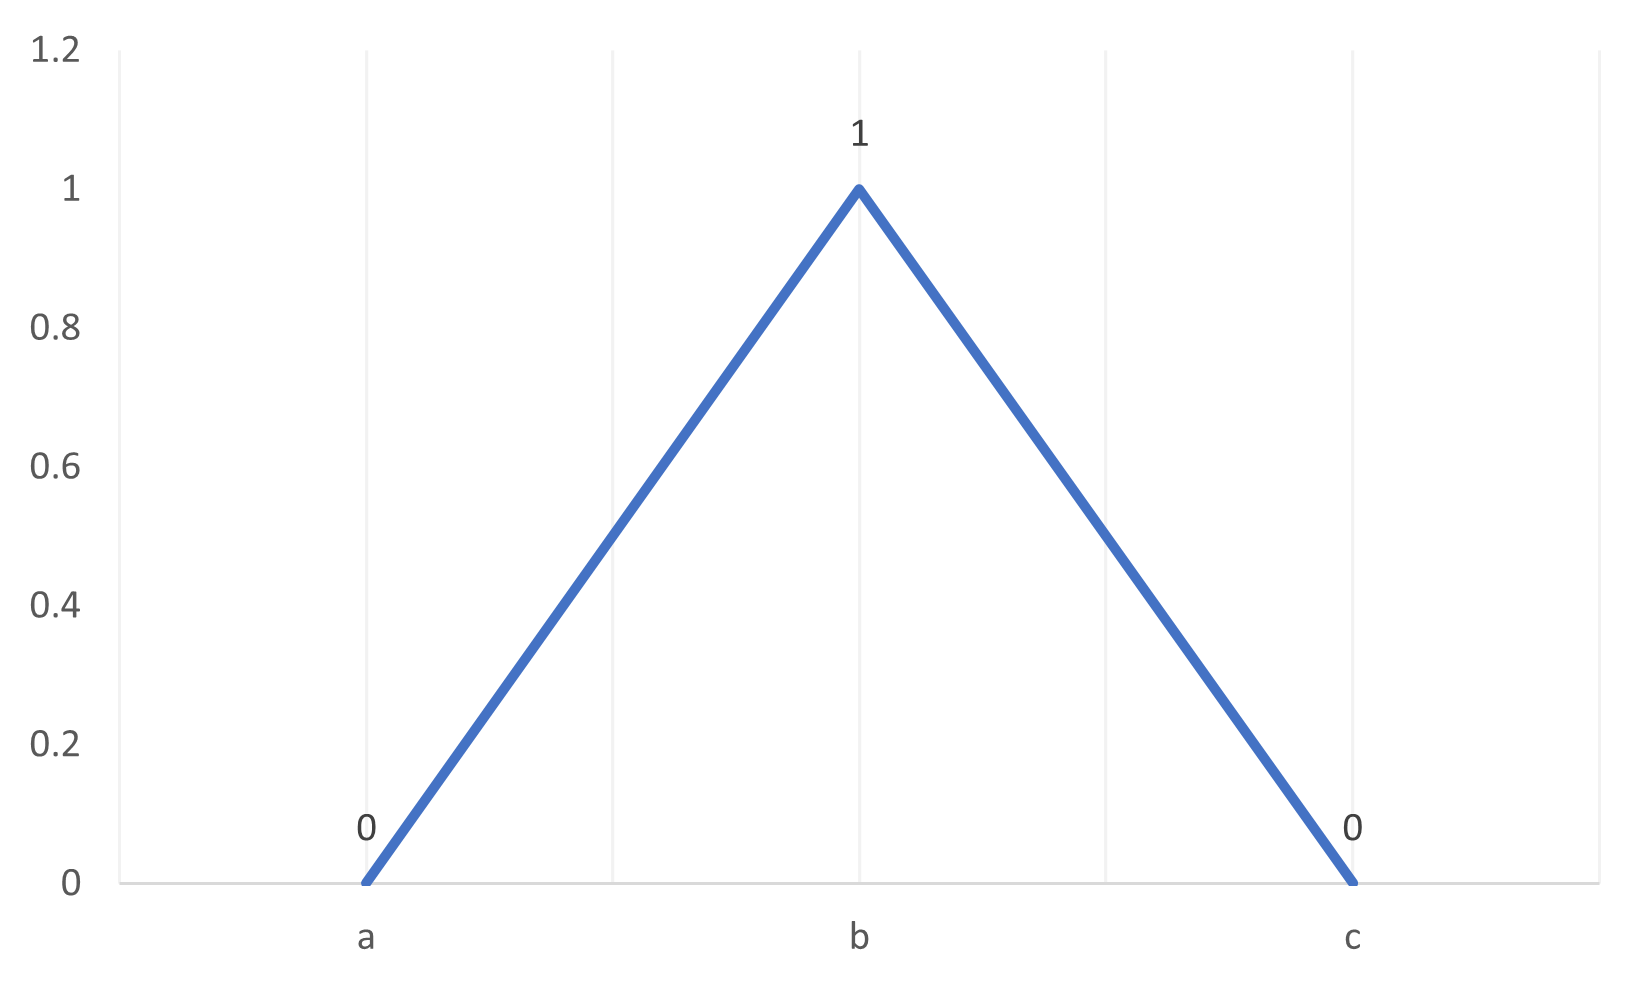
\includegraphics{figs/membership_tri.png}
%     }
%     \caption{三角隶属函数}
%     \label{fig:membership_tri}
%   \end{figure}

  \begin{figure}[htb]
    \centering
    \begin{minipage}[t]{0.49\linewidth}
      \centering
      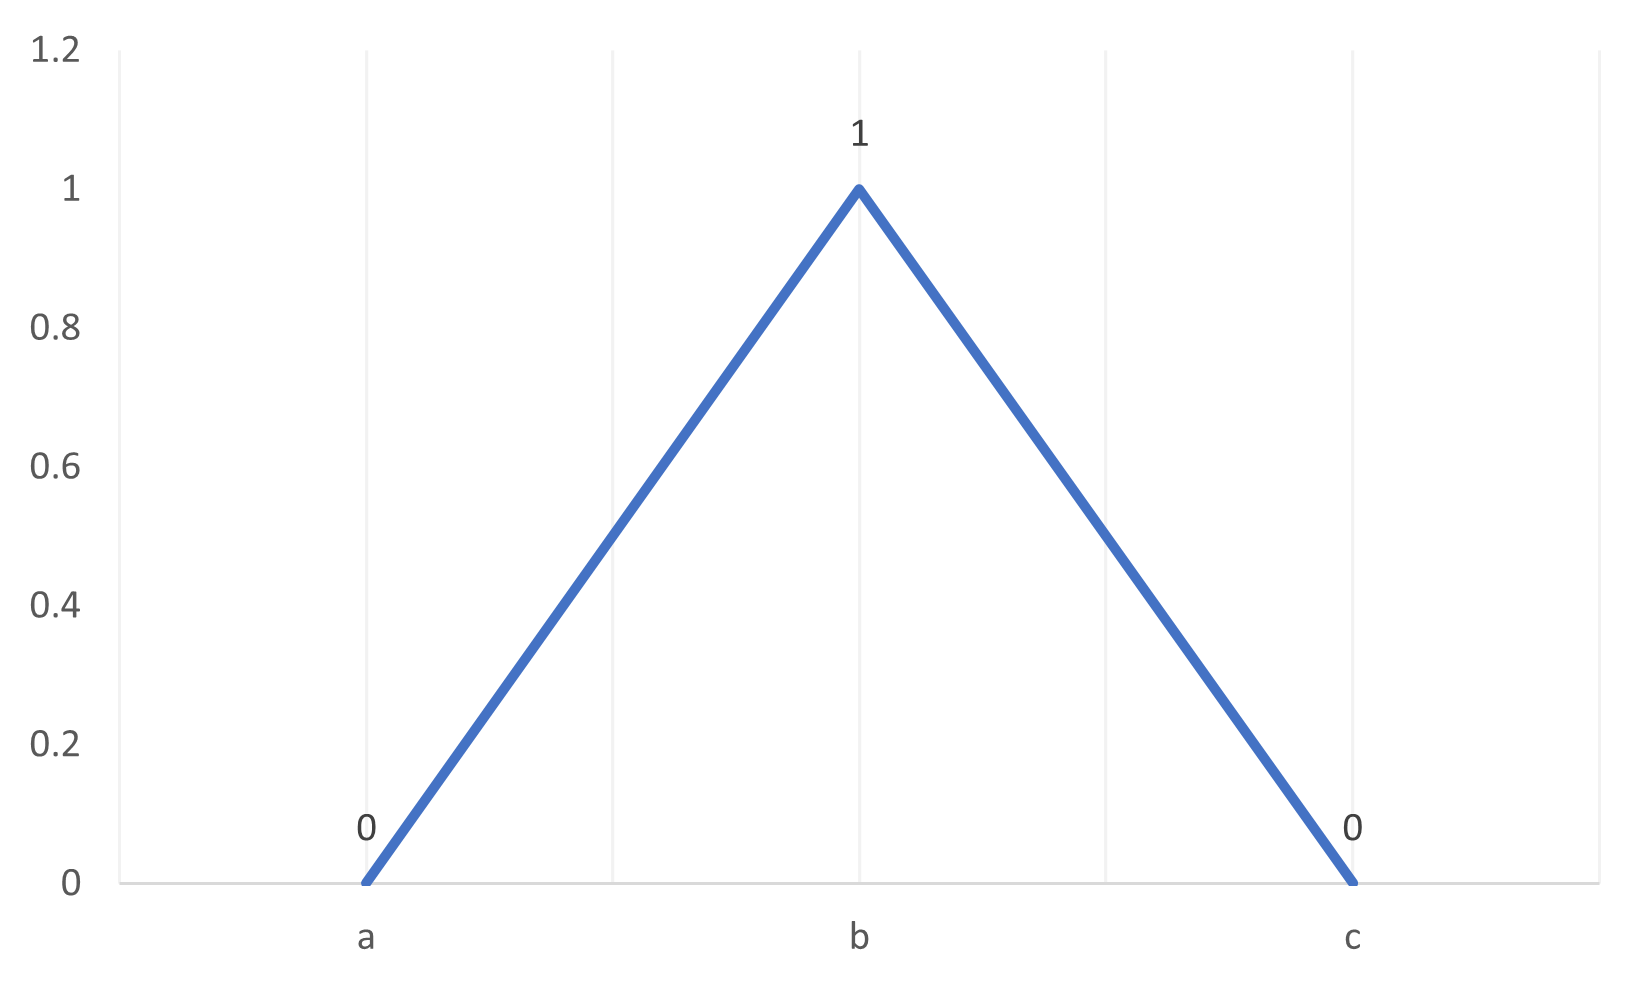
\includegraphics[width=\linewidth]{figs/membership_tri.png}
      \caption{三角隶属函数}
      \label{fig:membership_tri}
    \end{minipage}
    \hfill
    \begin{minipage}[t]{0.49\linewidth}
      \centering
      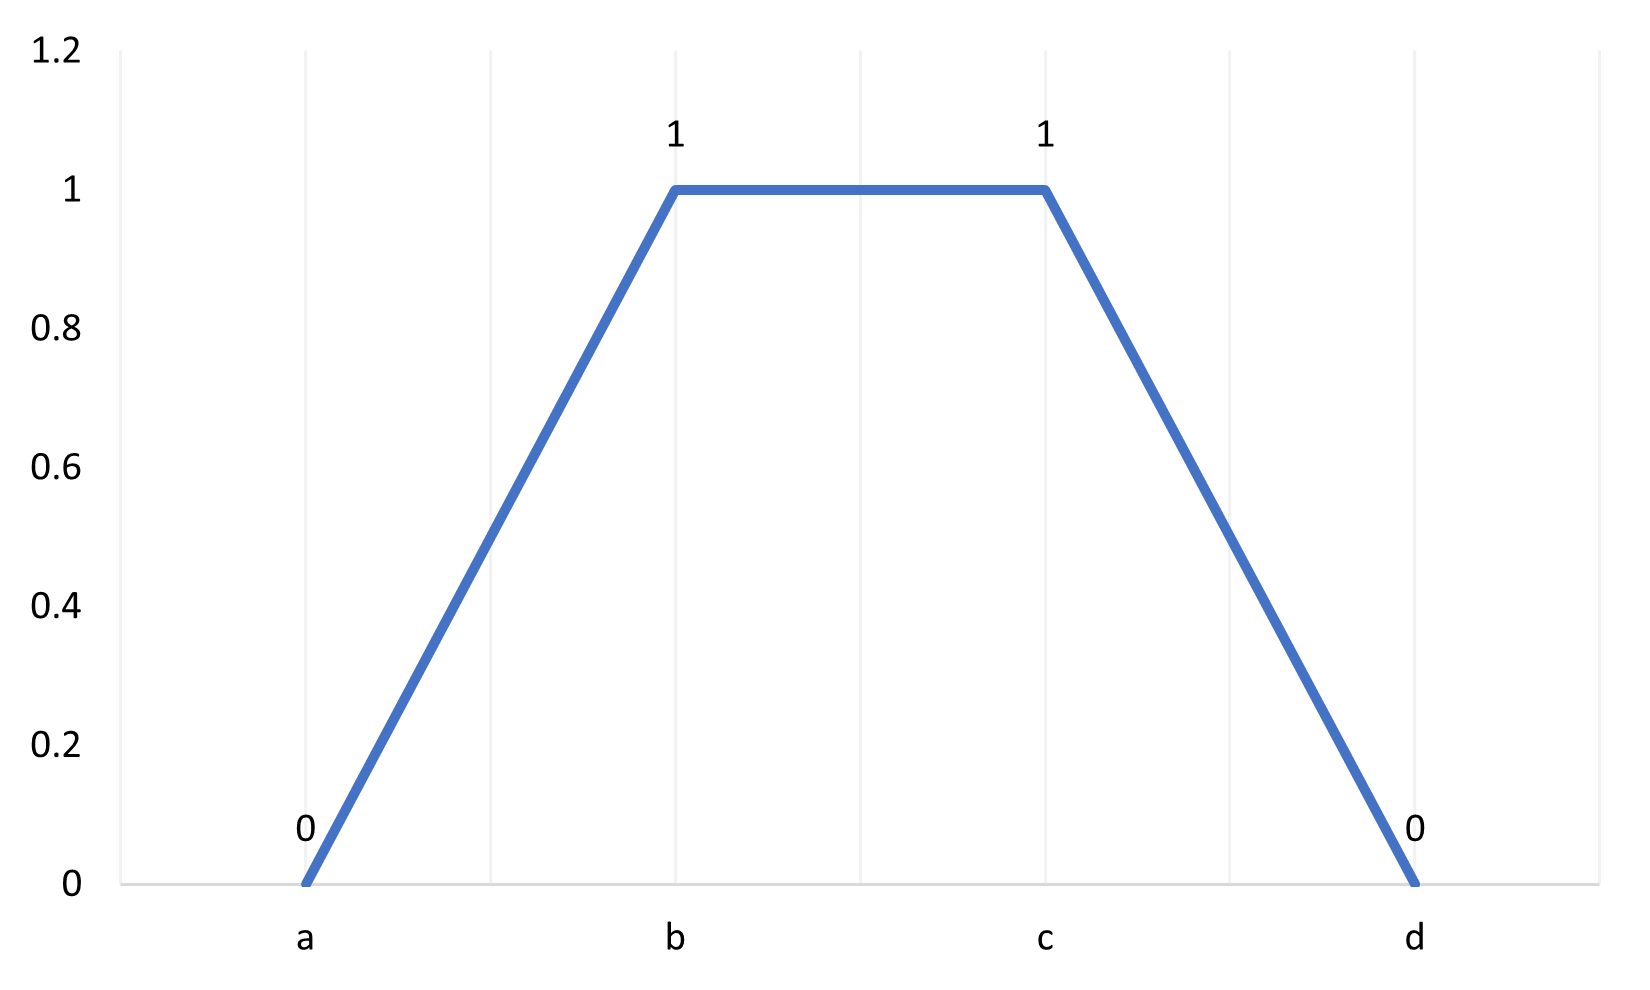
\includegraphics[width=\linewidth]{figs/membership_tixing.png}
      \caption{梯形隶属函数}
      \label{fig:membership_tixing}
    \end{minipage}
    \caption{常用模糊隶属函数}
    \label{fig:membership_function}
  \end{figure}

其中,横轴为任意对象$x$在属性$P$上的取值,纵轴为该对象隶属于该属性的模糊等价类的程度。其中三角隶属函数使少数对象的隶属度取到1,其余对象隶属度小于1。梯形隶属函数适用于落入区间$[b,c]$较多,从而可以使该区间内的对象的隶属度取到1。因而在实践中需要观察数据的分布及特点来确定模糊隶属函数\cite{基于粗糙集和模糊粗糙集的属性约简研究}。

% \begin{Definition}[模糊正域隶属度与模糊依赖度]
% 设$P \subseteq A$为条件属性子集, $Q\subseteq \{d\}$为决策属性子集, $X$是定义在$U$上的模糊集, 对于给定的对象$x$, 定义对象$x$属于模糊正域的隶属度为:

% $$\mu_{\operatorname{POS}_{P}^{R}(Q)}(x)=\sup _{X \in U / Q} \mu_{\underline{P} X}(x).$$

% 模糊条件属性$P$关于模糊决策属性$Q$的依赖度定义为:

% $$\tau_{P}(Q)=\frac{\sum_{x \in U} \mu_{P O S_{P}(Q)}(x)}{|U|} .$$
% \end{Definition}

% \begin{Definition}[正域]
% 设P和Q是在U上诱导等价关系的属性集, 则正域$\operatorname{POS}_{P}(Q)$, 负域$\operatorname{NEG}_{P}(Q)$和边界域$\operatorname{BND}_{P}(Q)$可以定义为:

%     $$\operatorname{POS}_{P}(Q) =\bigcup_{X \in \mathrm{U} / Q} \underline{P} X $$
%     $$\operatorname{NEG}_{P}(Q) =\mathbb{U}-\bigcup_{X \in \mathrm{U} / Q} \overline{P} X $$
%    $$ \operatorname{BND}_{P}(Q) =\bigcup_{X \in \mathrm{U} / Q} \overline{P} X-\bigcup_{X \in \mathrm{U} / Q} \underline{P} X $$

%    正域$\operatorname{POS}_{P}(Q)$包含$U$的所有对象, 这些对象可以使用属性$P$中的信息被分类为$U/Q$的类. 边界域$\operatorname{BND}_{P}(Q)$是可以但不一定可以以这种方式分类的对象的集合. 负域$\operatorname{NEG}_{P}(Q) $是一组不能分类为$U/Q$类的对象. 

% \end{Definition}
% 数据分析中的一个重要问题是发现属性之间的依赖关系。直观地说,如果来自$Q$的所有属性值由来自$P$的属性值唯一确定,那么就说明一组属性$Q$完全取决于一组属性$P$,记作$P \Rightarrow Q$。如果$Q$和$P$的值之间存在函数依赖性,那么$Q$完全依赖于$P$。

\section{属性约简算法}

属性约简算法是一种数据挖掘和特征选择的方法,用于从给定的属性集合中找到最小的子集,该子集保留了原始数据集的重要特征。它的目标是消除冗余和不必要的属性,以便在保持数据集表示能力的同时减少计算复杂性。通过约简属性集合,可以去除冗余的信息、降低存储和计算开销,避免过拟合的问题,同时能够更好地理解和解释数据。属性约简算法的基本思想是评估属性的重要性,根据事先设置好的约简准则选择最具有代表性和区分性的属性。这些准则可能基于信息论、统计学指标、启发式规则等。

粗糙集理论作为一种新的处理不精确、不确定和不完备数据的数学工具,目前已被广泛应用到数据挖掘、模式识别、特征选择等领域。粗糙集理论最主要的一个应用就是属性约简,该理论的成功部分归功于三个方面。首先,只分析数据中隐藏的事实。其次,在数据分析中不需要关于数据的附加信息,例如阈值或特定领域的专家知识。第三,它找到了数据的最小信息表示\cite{2009New}。因此在属性约简的研究中粗糙集有着非常广泛的应用。其中,基于粗糙集的属性方法根据决策表的类型与基于的方法不同都有着不同的分支。如\ref{fig:FuzzyRoughSetFeatureSelection}所示,基于粗糙集方法的属性约简算法主要分为基于不同类型决策信息表与基于不同方法两类。在基于不同方法的类别中,其中一种比较经典且普遍的算法为基于属性重要度的属性约简算法。该方法分别针对集合观与信息观有着两类不同的分支。

\begin{figure}[H]
    \centering
    \resizebox{\textwidth}{!}
    {
    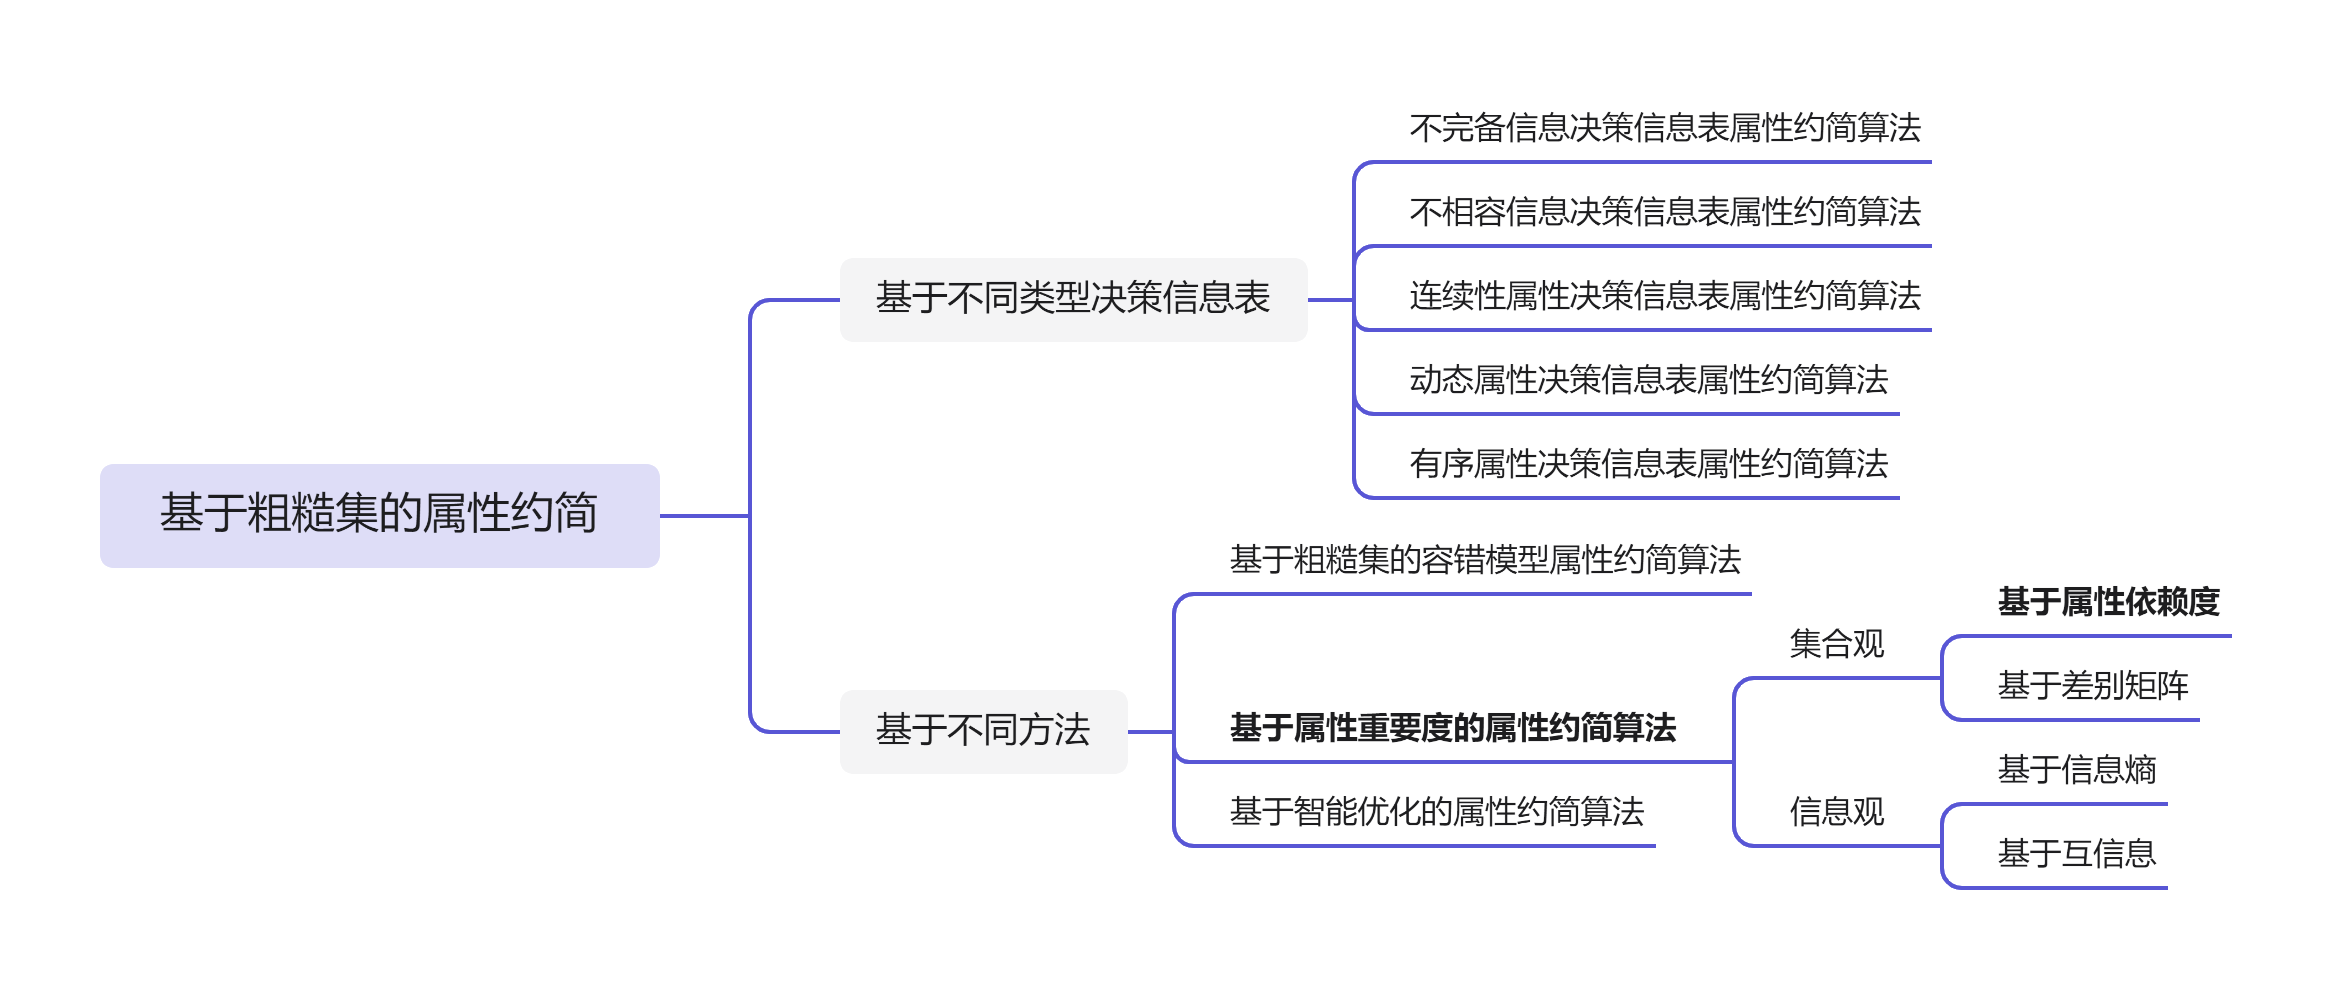
\includegraphics{figs/FuzzyRoughSetFeatureSelection.png}
    }
    \caption{基于粗糙集的属性约简算法}
    \label{fig:FuzzyRoughSetFeatureSelection}
  \end{figure}


由于本文的研究目标是利用粗糙集方法得到影响作物产量的主要影响因素,同时需要分析条件属性对于决策属性的的重要性,因此选择基于属性重要度的属性约简算法作为研究方法,同时选择属性依赖度作为属性重要度的计算方法。然而,经典粗糙集模型只能处理分类数据\cite{2020Information,Jianhua2017Neighbor}。在粮食生产数据数据中,大多数数据都是连续型数据,连续型数据在构造等价类过程中存在着困难。连续型数据往往需要离散化才能被粗糙集方法应用,但是离散化会导致原始数据携带的信息丢失\cite{2022Deep}。而基于模糊粗糙集方法的属性约简算法能够通过利用模糊隶属函数将连续值属性模糊化来刻画模糊等价类,可以克服其对于数据离散化要求的局限。因此,本文选择基于属性重要度的模糊粗糙集属性约简算法作为研究算法,并选择利用模糊依赖度刻画属性重要度,以此来作为特征选择方法对玉米产量影响因素进行分析。由于本文利用粗糙集方法对粮食生产数据进行处理的目的就是为了得到不同属性的重要度,因此在算法上只需要得到各个属性的重要度即可,无需再进行保持正域不变的条件下进行属性约简,因此本文算法仅选取到求出属性重要度为止,后续利用正域不变的条件逐步选出约简数据集的过程不在本文的研究范畴中。由\ref{section:粗糙集基本概念}中的理论知识,参考\cite{基于粗糙集和模糊粗糙集的属性约简研究}中提出的算法,可得到\nameref{alg:FRARAlgorithm}:

\begin{algorithm}[htbp]
    \caption{基于属性重要度的模糊粗糙集属性约简算法} %算法的名字
    \label{alg:FRARAlgorithm}
    \hspace*{0.02in} {\bf 输入:} %算法的输入, \hspace*{0.02in}用来控制位置,同时利用 \\ 进行换行
    信息系统$I=(U,C\cup D)$\\
    \hspace*{0.02in} {\bf 输出:} %算法的结果输出
    属性重要度$sig(C,D)$
    \begin{algorithmic}
        \State 利用模糊隶属函数对决策表进行连续属性模糊化
        \For{$\forall P \in C$} % For 语句,需要和EndFor对应
        \State 计算$P$在不同模糊划分$F_{ik}$中的模糊下近似$\mu_{\underline{P}}(F_{ik})$
        \For{$\forall x \in U$} % For 语句,需要和EndFor对应
                \State 计算每个对象$x$对该条件属性$P$的模糊正域的隶属度$\mu_{\operatorname{POS}}(x)$
        \EndFor
        \State 计算模糊条件属性$P$关于模糊决策属性$D$的模糊依赖度$\tau_{P}(D)$
        \State 得到模糊条件属性$P$关于模糊决策属性$D$的属性重要度$sig(P,D)$
        \EndFor
        \State 得到模糊条件属性集$C$关于模糊决策属性$D$的属性重要度$sig(C,D)$\\
    \Return 属性重要度$sig(C,D)$
    \end{algorithmic}
    \end{algorithm}



    % \begin{algorithm}[htbp]
    %   \caption{基于属性重要度的模糊粗糙集属性约简算法} %算法的名字
    %   \label{alg:FRARAlgorithm}
    %   \hspace*{0.02in} {\bf 输入:} %算法的输入, \hspace*{0.02in}用来控制位置,同时利用 \\ 进行换行
    %   信息系统$I=(U,C\cup D)$\\
    %   \hspace*{0.02in} {\bf 输出:} %算法的结果输出
    %   属性重要度$\operatorname{IMP}$
    %   \begin{algorithmic}
    %       \State 对决策表进行模糊模糊化
    %       \State 
    %       \While{$\operatorname{POS}_{A}(D)=\operatorname{POS}_{R}(D)$}
    %       \For{$\forall a \in C$} % For 语句,需要和EndFor对应
    %       \State 计算条件属性$a$与决策属性$D$的依赖度$DEP$
    %       \State 计算条件属性$a$的不可分辨系数$IND$
    %       \State 计算条件属性$a$的属性重要度$IMP=DEP-IND$
    %       \EndFor
    %       \State 选出属性重要度最大的属性$a'=\underset{a \in A-R}{\operatorname{argmax}}\left\{IMP\right\}$
    %       \State 更新约简属性集$R=R\cup \{a'\}$
    %       \EndWhile\\
    %   \Return $R \in \operatorname{RED}_{D}(A)$
    %   \end{algorithmic}
    %   \end{algorithm}

该算法输入为信息系统$I=(U,C\cup D)$,输出为条件属性集$C$中各个条件属性的属性重要度$sig(C,D)$。算法首先利用模糊隶属函数对决策表中的连续值属性进行模糊化,其中模糊等价类的个数需要事先通过聚类算法对数据进行聚类分析,以便得到恰当的模糊等价类个数,而模糊隶属函数的构造也需要依据数据集的分布及特点选择恰当的模糊隶属函数,一般情况下大都选择常用的三角隶属函数或梯形隶属函数。在得到由模糊隶属函数进行模糊化的决策表的同时也得到了相应的模糊划分$F_{ik}$。然后遍历条件属性集$C$中的每一个条件属性$P$,以计算其对于决策属性$D$的属性重要度$sig(P,D)$。属性重要度$sig(P,D)$由模糊依赖度$\tau_{P}(D)$定义,要计算每个条件属性的模糊依赖度,就要计算论域$U$中每个对象$x$对模糊正域的隶属度$\mu_{\operatorname{POS}}(x)$,要计算模糊正域隶属度$\mu_{\operatorname{POS}}(x)$,就要计算$F_{ik}$在决策属性$D$的模糊正域下的隶属度$\mu_{\operatorname{POS}}(F_{i k})$,因而需要计算$P$在不同模糊划分$F_{ik}$中的模糊下近似$\mu_{\underline{P}}(F_{ik})$。在每个对象$x$对模糊正域的隶属度$\mu_{\operatorname{POS}}(x)$的计算过程中,需要计算每个对象在各个模糊等价类下对每个决策类的隶属度,其中就涉及到$P$在不同模糊划分$F_{ik}$中的模糊下近似$\mu_{\underline{P}}(F_{ik})$。因此,在遍历条件属性集$C$中的每一个条件属性$P$时,先计算$P$在不同模糊划分$F_{ik}$中的模糊下近似$\mu_{\underline{P}}(F_{ik})$,然后为了计算模糊依赖度$\tau_{P}(D)$,遍历论域$U$中的每个对象$x$,计算$x$对模糊正域的隶属度$\mu_{\operatorname{POS}}(x)$。然后计算模糊条件属性$P$关于模糊决策属性$D$的模糊依赖度$\tau_{P}(D)$。进而得到模糊条件属性$P$关于模糊决策属性$D$的属性重要度$sig(P,D)$。在遍历结束后,就得到了模糊条件属性集$C$关于模糊决策属性$D$的属性重要度$sig(C,D)$,输出每个属性的重要度。


其中,对于模糊等价类个数的计算在本文实验中选择了模糊C均值聚类算法,对于模糊隶属函数的选择与构造需要根据数据分布及特点来确定,具体的过程将在\ref{chapter:基于属性重要度的模糊粗糙集属性约简算法}中进一步介绍。



% 为了解决这个问题,Dubois和Prade[12]通过结合模糊集[13]和粗糙集[1]定义了模糊粗糙集。由于模糊粗糙集可以有效降低数据的信息损失,提高模型的分类能力,因此模糊粗糙集及其扩展模型被广泛用于属性约简[14-16]和多属性决策[17,18]。


% 1992年,Kuncheva首次提出了一种使用模糊粗糙集的特征选择方法[38]。利用弱模糊划分方法定义了模糊的正、负和边界区域,提出了特征选择的思想。然而,由于FRS在当时刚刚诞生,它们并没有引起足够的关注。2004年,Jensen等人提出了一种基于FRS[39]的属性约简方法。从那时起,基于FRS的属性约简受到了广泛的关注。根据所使用的不同约简规则,基于FRS的属性约简方法可以大致可分为三类:(1)基于模糊依赖性的,(2)基于模糊不确定性测度的,以及(3)基于模糊辨别矩阵的。


% 现有关于模糊粗糙集的研究主要集中在模糊集的近似上。这些研究已经在[6]中进行了全面的研究和讨论。在[5]中,提出了一项关于模糊粗糙集属性约简的开创性工作。引入了模糊粗糙属性约简的形式化概念,并利用[5]中的依赖函数开发了一种计算约简的算法。



  

% 本文件是示例论文的一部分
% 论文的主文件位于上级目录的 `main.tex`

\chapter{粮食生产模型的建立与分析}

本章主要介绍全文建立的基于粗糙集方法的粮食生产模型,包括研究数据、模型框架、模型方法(特征选择方法、预测模型方法等)
\section{粮食生产数据}
\subsection{研究对象}
根据引言所述,本文选择了我国在2022年受到俄乌冲突影响最大的代表性主要农作物—玉米作为研究对象,通过利用粗糙集与其他经典特征选择方法筛选出影响其产量的主要影响因素,进而对我国农作物的生产与规划做出分析与建议。
\subsection{数据来源}
本文研究数据分别参考了《全国农产品成本收益资料汇编》与《中国农村统计年鉴》中各省农作物的生产数据与农村社会经济生产数据。其中在《全国农产品成本收益资料汇编》中选取了各省玉米历年与生产相关的生产数据,如每亩化肥用量、每亩种子用量等,反映的是作物在生产过程中的资源投入情况。在《中国农村统计年鉴》中选取了各省历年农村基本情况与生产状况的数据,如各省农业机械总动力、各省受灾面积等,反映的是各省农村生产条件与状况。
\subsection{数据范围}
本文研究数据在时间尺度上选择了《全国农产品成本收益资料汇编》与《中国农村统计年鉴》在2004-2021年的数据,空间尺度上选择了以上两个数据集中关于玉米生产所共有的19个主要农业大省的数据,具体见下表:
\[
\text{空间尺度}
\begin{cases}
\text{东北地区:辽宁、吉林、黑龙江}\\
\text{华北地区:河北、山西、内蒙古}\\
\text{华东地区:江苏、安徽、山东}\\
\text{中南地区:河南、湖北}\\
\text{西南地区:四川、重庆、贵州、云南}\\
\text{西北地区:陕西、甘肃、宁夏、新疆}
\end{cases}
\]

\begin{figure}[htbp]
  \centering
  \resizebox{\textwidth}{!}
  {
  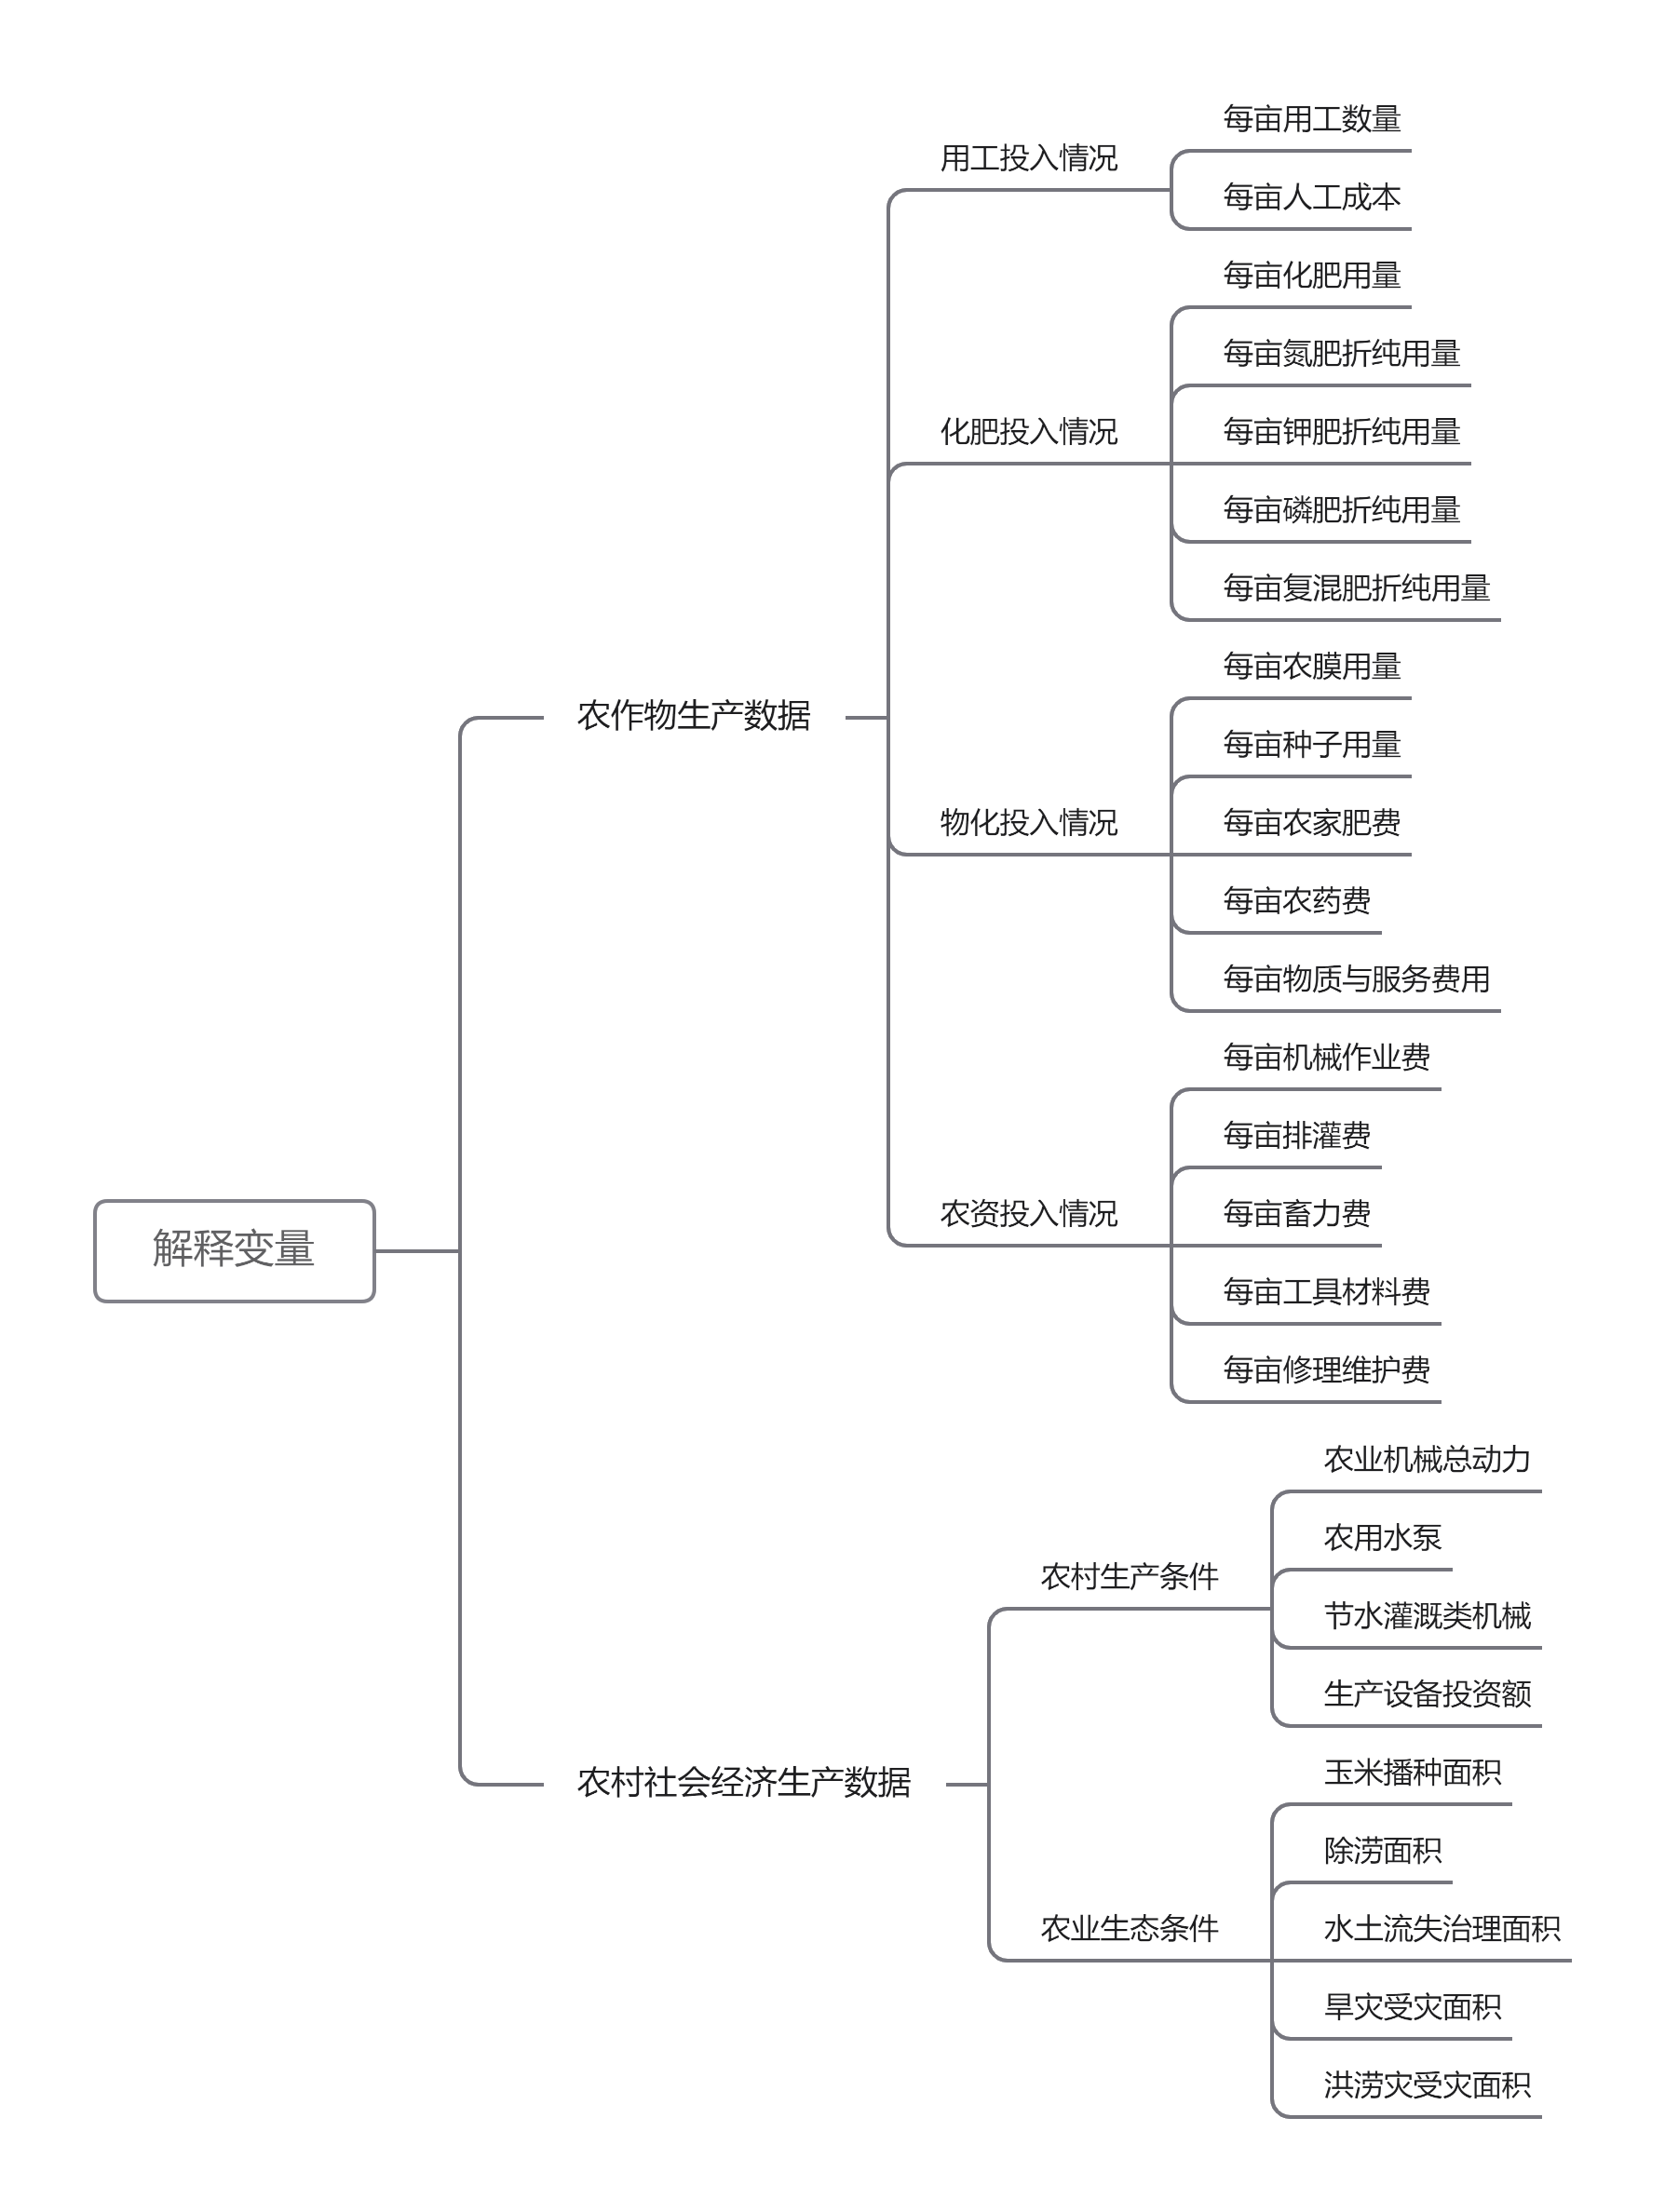
\includegraphics{figs/explanatory_variable.png}
  }
  \caption{26个玉米生产解释变量}
  \label{fig:explanatory_variable}
\end{figure}


\subsection{研究变量}
本文研究中,被解释变量选为各省历年每亩玉米的产量,解释变量共计26个,分别选自《全国农产品成本收益资料汇编》与《中国农村统计年鉴》中与作物生产相关的各方面数据,其中《全国农产品成本收益资料汇编》中选择的解释变量均为各省历年仅投入到每亩玉米土地的数据,而非所有粮食作物的宏观统计数据,所有解释变量见\ref{fig:explanatory_variable}。


% \[
% \text{解释变量}
% \begin{cases}
% \text{  农作物生产数据  }
% \begin{cases}
%   \text{用工投入情况}
%   \begin{cases}
%     \text{每亩用工数量}\\
%     \text{每亩人工成本}
%   \end{cases}\\
%   \text{化肥投入情况}
%   \begin{cases}
%     \text{每亩化肥用量}\\
%     \text{每亩氮肥折纯用量}\\
%     \text{每亩钾肥折纯用量}\\
%     \text{每亩磷肥折纯用量}\\
%     \text{每亩复混肥折纯用量}\\
%   \end{cases}\\
%   \text{物化投入情况}
%   \begin{cases}
%     \text{每亩农膜用量}\\
%     \text{每亩种子用量}\\
%     \text{每亩农家肥费}\\
%     \text{每亩农药费}\\
%     \text{每亩物质与服务费用}
%   \end{cases}\\
%   \text{农资投入情况}
%   \begin{cases}
%     \text{每亩机械作业费}\\
%     \text{每亩排灌费}\\
%     \text{每亩畜力费}\\
%     \text{每亩工具材料费}\\
%     \text{每亩修理维护费}\\
%   \end{cases}\\
%   \end{cases}\\
% \text{农村社会经济生产数据}
% \begin{cases}
% \text{农村生产条件}
% \begin{cases}
%   \text{农业机械总动力}\\
%   \text{农用水泵}\\
%   \text{节水灌溉类机械}\\
%   \text{生产设备投资额}\\
% \end{cases}\\
% \text{农业生态条件}
% \begin{cases}
%   \text{玉米播种面积}\\
%   \text{除涝面积}\\
%   \text{水土流失治理面积}\\
%   \text{旱灾受灾面积}\\
%   \text{洪涝灾受灾面积}\\
% \end{cases}
% \end{cases}
% \end{cases}
% \]




% \DTLloaddb{Data}{data/Data.csv}
% \begin{table}[htbp]
%       \centering
%       \caption{玉米生产数据:陕西省}
%       \label{table:Data}
%       \resizebox{\textwidth}{!}
%       {
%       \csvautobooktabular{data/Data.csv}
%       }
% \end{table}

\subsection{数据预处理}
\label{subsection:DataCleaning}
在本文的研究中,对于某些省份个别年份中出现的空值数据选择了零值填充法进行填充。同时为了构造模糊环境,选择了大多数研究中采取的线性函数归一化方法对数据进行预处理\cite{BestOverview},以便后续利用模糊粗糙集属性约简算法进行特征选择。
\section{粮食生产模型}
本节主要介绍本文建立的粮食生产模型,以便能够利用粮食生产模型对粮食安全进行分析。
\subsection{模型框架}
本模型主要由三个主体部分组成,第一部分为特征选择模型,第二部分为预测模型,第三部分对粮食安全进行可视化分析。第一部分的特征选择模型主要用于对解释变量进行筛选,以便得出最重要的解释变量;第二部分的预测模型主要用于对第一部分特征选择模型的结果进行评估与实验分析,以便分析粗糙集方法相对于其他经典特征选择方法的优劣;第三部分对模糊粗糙集属性约简算法得到的结果进行可视化分析,以便对我国玉米生产及粮食安全提供建议。模型框架见\ref{fig:FoodProductionModel}。


\begin{figure}[htbp]
  \centering
  \resizebox{\textwidth}{!}
  {
  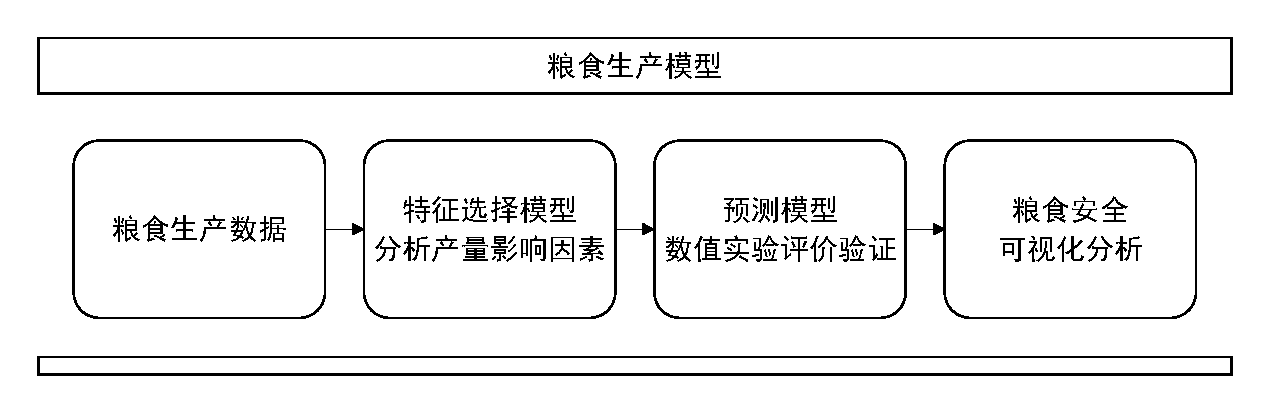
\includegraphics{figs/FoodProductionModel}
  }
  \caption{粮食生产模型框架}
  \label{fig:FoodProductionModel}
\end{figure}


\subsection{特征选择模型}
特征选择模型分别利用了三种不同的特征选择方法:基于属性重要度的模糊粗糙集属性约简算法、基于回归模型的Lasso特征选择算法、基于随机森林模型的随机森林变量重要性算法,通过分别利用以上三种特征选择方法对数据进行特征选择,分别得出不同方法下最重要的10个解释变量,然后再分别将原数据集按照不同特征选择方法得出的特征选择结果进行属性约简,删掉不同方法下重要性排名不在前10的解释变量,分别得到经过三种不同特征选择方法处理后的约简数据集,其中约简后的数据集中只保留了不同特征选择方法下最重要的10个解释变量,以期能够达到在保持分类能力不变的情况下尽可能约简数据集的目的。

\subsection{预测模型}
预测模型在特征选择模型的基础上,通过将不同特征选择模型处理后的约简数据集以及未约简数据集放入预测模型进行预测,以便比较不同数据集在训练误差、训练时间、测试误差、预测精度方面的优劣,进而分析出不同特征选择方法在特征选择方面的差异。

在具体数值实验中,本文选择利用随机森林模型作为预测模型,将各省2004-2020年的约简数据集作为训练数据对模型进行训练,再将各省2021年的粮食单产产量作为预测数据,通过比较预测产量与真实产量之间的差距,进而评估该数据集的预测精度。然而由于预测模型为随机森林模型,理论上特征选择方法中的随机森林变量重要性算法得到的约简数据集对于随机森林预测模型的拟合效果是最好的,因而其在误差、耗时、精度等各方面表现应该较优,因而可以将随机森林变量重要性算法得到的结果作为一个统一的参考,进而可以比较出Lasso算法和粗糙集算法的效果。

\subsection{粮食安全分析}

针对特征选择与预测模型的结果,采用FRAR作为特征选择方法,得到每个省份影响玉米产量的前10个解释变量。并针对相对较为重要的变量从化肥投入情况、成本投入情况、排灌建设情况及机械化建设情况4个方面分别进行了结果可视化,并对特征选择结果进行了分析,为我国玉米生产与粮食安全提供了建议。

%%%%%%%%%%%%%%%%%%%%%%%%%%%%%%%%%%%%%%%%%%%%%%%%%%%%%%%%%%%%%%%%%%%%%%
% \section{插图}

% \subsection{直接插图}
% 使用xelatex命令编译时,\LaTeX{}支持\verb|.pdf|和\verb|.eps|格式的矢量图,
% 也支持\verb|.jpg|、\verb|.png|或\verb|.bmp|格式的位图,当然也可以在\LaTeX{}
% 中直接绘图,关于插图图片推荐的方式有:

% \begin{enumerate}
% \item 使用其它绘图工具绘图生导出或打印成 \verb|pdf| 格式的\emph{矢量图}。
% \item 使用\LaTeX{}的宏包来绘制插图,如 \pkg{Ti\textit{k}Z},它兼容所有 \LaTeX{} 环境,
% 字体能与全文统一,质量最佳,但是需要的学习成本较大。
% 请务必先阅读 \pkg{Ti\textit{k}Z} 文档教程,
% 然后可以去 texample\footnote{\url{http://texample.net/tikz}} 等网站上找类似的例子,
% \item 利用截图工具生成位图,不过\emph{质量堪忧},小心遭批。
% \item 对于现场照片等只能用相机等设备拍照成位图插入,小心遭批。
% \item 最后,一般论文都是\emph{单色印刷}的,请确保插图在黑白打印情况下的清晰度。
% \end{enumerate}

% % \begin{figure}[!htb]
% %   \centering
% %   \newcounter{density}
% %   \setcounter{density}{20}
% %   \begin{tikzpicture}[font=\small]
  \def\couleur{orange}
  \path[coordinate] (0,0) coordinate(A)
              ++( 90:4cm) coordinate(B)
              ++(0:4cm) coordinate(C)
              ++(-90:4cm) coordinate(D);
  \draw (A) node[left] {A}
    (B) node[left] {B}
    (C) node[right] {Point C} --
    (D) node[right,midway,align=left] {边长$a$ \\ 面积和:$S=\frac{50}{9}a^2$ \\ 边长和:$C=\frac{20}{9}(10+\sqrt{82})a$}
    node[right] {点D};
  \draw[fill=\couleur!\thedensity] (A)--(B)--(C)--(D)--cycle;
  \foreach \x in {1,...,40}{%
      \pgfmathsetcounter{density}{\thedensity+25}
      \setcounter{density}{\thedensity}
      \path[coordinate] coordinate(X) at (A){};
      \path[coordinate] (A) -- (B) coordinate[pos=.1](A)
                          -- (C) coordinate[pos=.1](B)
                          -- (D) coordinate[pos=.1](C)
                          -- (X) coordinate[pos=.1](D);
      \draw[fill=\couleur!\thedensity] (A)--(B)--(C)--(D)--cycle;
  }
\end{tikzpicture}

% %   \caption{在\LaTeX{}中直接用Ti\textit{k}Z绘制的矢量图}
% %   \label{fig:tikzrot}
% % \end{figure}

% \begin{figure}[!htb][H]
%   \centering
%   
\includegraphics[width=4.1cm]{nwafu-circle}
%   \caption{CorelDraw绘制导出的校徽PDF矢量图}
%   \label{fig:logo}
% \end{figure}


% \subsection{子图排版}

% 如需要多个子图共用一个题注,需加载额外宏包,可以使用\pkg{subcaption}等宏包实现,
% 如\autoref{fig:sub2}所示。若需要更为复杂的子图控制,个人推荐使用\pkg{floatrow}
% 宏包实现更为复杂和灵活的子图排版中的细节控制。

% \begin{figure}[!htb]
%   \centering
%   \subfloat[左边的大校徽\label{fig:sub1}]{
%     
\includegraphics[width=2.8cm]{nwafu-circle}
%   }\quad
%   \subfloat[短标题:小校徽][小校徽,题注很长,不过请各位放心,它会自动换行\label{fig:sub2}]
%   {
%     
\includegraphics[width=4.6cm]{nwafu-bar}
%   }
%   \caption{用subcaption宏包排版子图}
%   \label{fig:subfigs}
% \end{figure}

% 强烈建议使用\emph{矢量图}图片,获得矢量图的一种方式是是直接使用
% \LaTeX{}的绘制宏包\pkg{Ti\textit{k}Z}、\pkg{pgfplots}等宏包进行绘制,另一
% 种获取矢量图的方式是用Matplotlib、MatLab、Mathematica、Python等工具绘图后
% 导出pdf格式的矢量图。如\ref{fig:plots}所示。

% \begin{figure}[htb]
%   \centering
%   \subfloat[二维图像\label{fig:func}]
%     {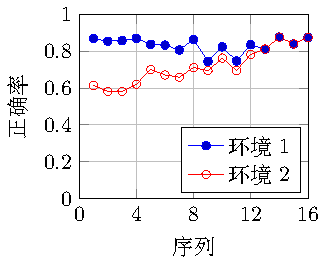
\includegraphics[scale=0.65]{figs/plot_2d}} \qquad
%   \subfloat[三维图像\label{fig:sum}]
%     {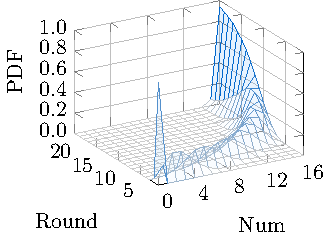
\includegraphics[scale=0.65]{figs/plot_3d}}
%   \caption{利用 \pkg{pgfplot} 绘图}
%   \label{fig:plots}
% \end{figure}
% %

% \subsection{双语题注排版}

% 在研究生学位论文中,需使用双语题注(中文和英文),为此,本模板选用
% \pkg{bicaption}宏包实现双语题注,其效果可以参考\ref{fig:bicap}。当然,
% 也可以使用其它宏包实现双语题注排版,请大家根据情况自行处理。

% \begin{figure}[!htb]
%   \centering
%   
\includegraphics[width=4.2cm]{nwafu-bar}
%   \bicaption{双语题注}{bilingual caption}
%   \label{fig:bicap}
% \end{figure}

% \subsection{超宽插图排版(卧图)}

% 如果需要插入图片超出了页面宽度,建议使用\emph{卧排}的方式实现排版,一种常
% 用的方式是使用 \pkg{lscape}宏包提供的 \env{landscape}环境进行排版。效果参
% 见\ref{fig:fullpage1}。

% \setcounter{subfigure}{0}
% \begin{landscape}
% \vspace*{\fill} % 填充空白
% \begin{figure}[!hb]
%   \centering
%   \subfloat[First caption\label{fig:fp1}]
%     {
\includegraphics[width=.8\textheight]{nwafu-bar}} \\
%   \subfloat[Second caption]
%     {
\includegraphics[height=2cm]{nwafu-bar}}
%   \caption{用\emph{卧排}实现超宽插图排版}
%   \label{fig:fullpage1}
% \end{figure}
% \vspace*{\fill} % 填充空白
% \end{landscape}

% \section{表格}

% \subsection{内置表格排版环境}

% 对于简单的表格,可以使用\LaTeX{}内置的 \env{tabular} 环境实现排版,
% 如\ref{tab:city}。

% \begin{table}[htb]
%   \centering
%   \caption[城市人口]{城市人口数量排名 (source: Wikipedia)\label{tab:city}}
%   \begin{tabular}{lr}
%     \toprule
%     \multicolumn{1}{c}{城市} & \multicolumn{1}{c}{人口} \\
%     \midrule
%     Mexico City              & 20,116,842               \\
%     Shanghai                 & 19,210,000               \\
%     Peking                   & 15,796,450               \\
%     Istanbul                 & 14,160,467               \\
%     \bottomrule
%   \end{tabular}
% \end{table}

% \note{在学位论文中,表格要求采用三线表},因此,需要使用\pkg{booktabs}宏包
% 提供的\cs{toprule}、\cs{midrule}和\cs{bottomrule}分别绘制表格的顶线、中线
% 和底线。

% \subsection{表格浮动体}

% 由于学位论文中表格数量较多,且表格内容(长度)变化较大,当表格过长(一页内)时,
% 可能会带来分页困难,与插图类似,\LaTeX{}引入的\emph{浮动体}机制,可以使表格
% 脱离上下文,自动布置于合适的位置,从而避免在排版中产生留白问题。对于表格,
% 浮动体是通过\env{table}环境实现的。同时,利用\env{table}环境还能够较好地实
% 现插图编号及交叉引用的自动化。

% \subsection{跨页长表格}

% 如果表格内容很多,导致无法放在一页内的话,则需要用 \env{longtable}宏包实现
% 表格的跨页排版,如\ref{tab:performance}所示(数据来自南京航空航天大学毕业论
% 文\LaTeX{}模板)。

% % 定义表中用到的的宏,以简化表格代码并为后续修改提供统一接口
% \def\tabcaption{实验数据}
% \def\tabheadrow{
%   \multirow{2}{*}{测试程序} & \multicolumn{1}{c}{正常运行} &
%    \multicolumn{1}{c}{同步} & \multicolumn{1}{c}{检查点} &
%    \multicolumn{1}{c}{卷回恢复} & \multicolumn{1}{c}{进程迁移} &
%    \multicolumn{1}{c}{检查点} \\
%    & \multicolumn{1}{c}{时间(s)} & \multicolumn{1}{c}{时间(s)} &
%    \multicolumn{1}{c}{时间(s)} & \multicolumn{1}{c}{时间(s)} &
%    \multicolumn{1}{c}{时间(s)} & \multicolumn{1}{c}{文件(KB)} \\
%  }

% % 定义跨页表续表表题
% \def\ctntabcap{
%    \caption* {表~\thetable\hskip1em 实验数据(续)}\\
%    \addlinespace[-3.0ex]
%  }
% % 定义跨页表命令集合
% \def\ctntabcmd{
%    \ctntabcap\\
%    \toprule
%    \tabheadrow
%    \midrule
%    \endhead
%    \midrule
%    \multicolumn{7}{r}{\small 接下页}\\
%    \endfoot
%    \endlastfoot
%  }

% \begin{longtable}[c]{c*{6}{r}}
%   \caption[实验数据]{\tabcaption}\label{tab:performance}\\
%   \toprule
%   \tabheadrow
%   \midrule
%   \endfirsthead
%   \ctntabcmd
%   CG.A.2 & 23.05 & 0.002 & 0.116 & 0.035 & 0.589 & 32491 \\
%   CG.A.4 & 15.06 & 0.003 & 0.067 & 0.021 & 0.351 & 18211 \\
%   CG.A.8 & 13.38 & 0.004 & 0.072 & 0.023 & 0.210 & 9890 \\
%   CG.B.2 & 867.45 & 0.002 & 0.864 & 0.232 & 3.256 & 228562 \\
%   CG.B.4 & 501.61 & 0.003 & 0.438 & 0.136 & 2.075 & 123862 \\
%   CG.B.8 & 384.65 & 0.004 & 0.457 & 0.108 & 1.235 & 63777 \\
%   MG.A.2 & 112.27 & 0.002 & 0.846 & 0.237 & 3.930 & 236473 \\
%   MG.A.4 & 59.84 & 0.003 & 0.442 & 0.128 & 2.070 & 123875 \\
%   MG.A.8 & 31.38 & 0.003 & 0.476 & 0.114 & 1.041 & 60627 \\
%   MG.B.2 & 526.28 & 0.002 & 0.821 & 0.238 & 4.176 & 236635 \\
%   MG.B.4 & 280.11 & 0.003 & 0.432 & 0.130 & 1.706 & 123793 \\
%   MG.B.8 & 148.29 & 0.003 & 0.442 & 0.116 & 0.893 & 60600 \\
%   LU.A.2 & 2116.54 & 0.002 & 0.110 & 0.030 & 0.532 & 28754 \\
%   LU.A.4 & 1102.50 & 0.002 & 0.069 & 0.017 & 0.255 & 14915 \\
%   LU.A.8 & 574.47 & 0.003 & 0.067 & 0.016 & 0.192 & 8655 \\
%   LU.B.2 & 9712.87 & 0.002 & 0.357 & 0.104 & 1.734 & 101975 \\
%   LU.B.4 & 4757.80 & 0.003 & 0.190 & 0.056 & 0.808 & 53522 \\
%   CG.B.2 & 867.45 & 0.002 & 0.864 & 0.232 & 3.256 & 228562 \\
%   CG.B.4 & 501.61 & 0.003 & 0.438 & 0.136 & 2.075 & 123862 \\
%   CG.B.8 & 384.65 & 0.004 & 0.457 & 0.108 & 1.235 & 63777 \\
%   MG.A.2 & 112.27 & 0.002 & 0.846 & 0.237 & 3.930 & 236473 \\
%   MG.A.4 & 59.84 & 0.003 & 0.442 & 0.128 & 2.070 & 123875 \\
%   MG.A.8 & 31.38 & 0.003 & 0.476 & 0.114 & 1.041 & 60627 \\
%   MG.B.2 & 526.28 & 0.002 & 0.821 & 0.238 & 4.176 & 236635 \\
%   MG.B.4 & 280.11 & 0.003 & 0.432 & 0.130 & 1.706 & 123793 \\
%   LU.A.2 & 2116.54 & 0.002 & 0.110 & 0.030 & 0.532 & 28754 \\
%   LU.A.8 & 574.47 & 0.003 & 0.067 & 0.016 & 0.192 & 8655 \\
%   LU.B.2 & 9712.87 & 0.002 & 0.357 & 0.104 & 1.734 & 101975 \\
%   LU.B.8 & 2444.05 & 0.004 & 0.222 & 0.057 & 0.548 & 30134 \\
%   EP.A.2 & 123.81 & 0.002 & 0.010 & 0.003 & 0.074 & 1834 \\
%   EP.A.8 & 31.06 & 0.004 & 0.017 & 0.005 & 0.073 & 1661 \\
%   EP.B.2 & 495.49 & 0.001 & 0.009 & 0.003 & 0.196 & 2011 \\
%   EP.B.8 & 126.74 & 0.003 & 0.017 & 0.005 & 0.083 & 1656 \\
%   \bottomrule
% \end{longtable}

% \subsection{表格的双语题注}

% 在研究生学位论文中,需使用双语题注(中文和英文),为此,本模板选用
% \pkg{bicaption}宏包实现双语题注,其效果可以参考\ref{tab:bicap}。当然,
% 也可以使用其它宏包实现双语题注排版,请大家根据情况自行处理。

% \begin{table}[htb]
%   \centering
%   \bicaption[城市人口]{城市人口数量排名 (source:
%     Wikipedia)\label{tab:bicap}}{Urban population ranking}
%   \begin{tabular}{lr}
%     \toprule
%     \multicolumn{1}{c}{城市} & \multicolumn{1}{c}{人口} \\
%     \midrule
%     Mexico City              & 20,116,842               \\
%     Shanghai                 & 19,210,000               \\
%     Peking                   & 15,796,450               \\
%     Istanbul                 & 14,160,467               \\
%     \bottomrule
%   \end{tabular}
% \end{table}

% \subsection{超宽表格排版(卧表)}

% 如果需要插入超出页面宽度的表格,可以使用\pkg{lscape}宏包提供的 \env{landscape}
% 环境排版\emph{卧表},效果参见\ref{tab:toowidetab}。

% \begin{landscape}
% \vspace*{\fill} % 填充空白
% \begin{table}[!htb]
%   \centering
%   \caption{Laser specifications}
%   \label{tab:toowidetab}
%   \begin{tabular}{ccccccccc}
%     \toprule
%     Wavelength & Model & Package & Emmitter type & Manufacturer & Power (mW) & Iop (mA) & Ith (mA) & Vop (V)\\
%     \midrule
%     405 & DL-7386-101HG & TO-56 & single & sanyo & 50-70 & 70 & 35 & 4.8\\
%     450 & PL 450 & TO-38 & single & osram & 50-90 & 120 & 30 & 5.5\\
%     638 & ML520G54 & TO-56 & single & mitsubishi & 90-100 & 150 & 50 & 2.7\\
%     655 &  DL-5147-242 & TO-56 & single & sanyo & 30-50 & 80 & 40 & 3.8\\
%     \bottomrule
%   \end{tabular}
% \end{table}
% \vspace*{\fill} % 填充空白
% \end{landscape}

% 如果需要插入超宽超长表格,可以使用\pkg{lscape}宏包提供的 \env{landscape}
% 结合\env{longtable}环境排版\emph{跨页卧表},效果参见\ref{tab:landscapeperformance}。

% \begin{landscape} 
%   \begin{longtable}[c]{c*{6}{r}}
%     \caption[实验数据]{\tabcaption}\label{tab:landscapeperformance}\\
%     \toprule
%     \tabheadrow
%     \midrule
%     \endfirsthead
%     \ctntabcmd
%     CG.A.2 & 23.05 & 0.002 & 0.116 & 0.035 & 0.589 & 32491 \\
%     CG.A.4 & 15.06 & 0.003 & 0.067 & 0.021 & 0.351 & 18211 \\
%     CG.A.8 & 13.38 & 0.004 & 0.072 & 0.023 & 0.210 & 9890 \\
%     CG.B.2 & 867.45 & 0.002 & 0.864 & 0.232 & 3.256 & 228562 \\
%     CG.B.4 & 501.61 & 0.003 & 0.438 & 0.136 & 2.075 & 123862 \\
%     CG.B.8 & 384.65 & 0.004 & 0.457 & 0.108 & 1.235 & 63777 \\
%     MG.A.2 & 112.27 & 0.002 & 0.846 & 0.237 & 3.930 & 236473 \\
%     MG.A.4 & 59.84 & 0.003 & 0.442 & 0.128 & 2.070 & 123875 \\
%     MG.A.8 & 31.38 & 0.003 & 0.476 & 0.114 & 1.041 & 60627 \\
%     MG.B.2 & 526.28 & 0.002 & 0.821 & 0.238 & 4.176 & 236635 \\
%     MG.B.4 & 280.11 & 0.003 & 0.432 & 0.130 & 1.706 & 123793 \\
%     MG.B.8 & 148.29 & 0.003 & 0.442 & 0.116 & 0.893 & 60600 \\
%     LU.A.2 & 2116.54 & 0.002 & 0.110 & 0.030 & 0.532 & 28754 \\
%     LU.A.4 & 1102.50 & 0.002 & 0.069 & 0.017 & 0.255 & 14915 \\
%     LU.A.8 & 574.47 & 0.003 & 0.067 & 0.016 & 0.192 & 8655 \\
%     LU.B.2 & 9712.87 & 0.002 & 0.357 & 0.104 & 1.734 & 101975 \\
%     LU.B.4 & 4757.80 & 0.003 & 0.190 & 0.056 & 0.808 & 53522 \\
%     LU.B.8 & 2444.05 & 0.004 & 0.222 & 0.057 & 0.548 & 30134 \\
%     CG.B.2 & 867.45 & 0.002 & 0.864 & 0.232 & 3.256 & 228562 \\
%     CG.B.4 & 501.61 & 0.003 & 0.438 & 0.136 & 2.075 & 123862 \\
%     CG.B.8 & 384.65 & 0.004 & 0.457 & 0.108 & 1.235 & 63777 \\
%     MG.A.2 & 112.27 & 0.002 & 0.846 & 0.237 & 3.930 & 236473 \\
%     MG.A.4 & 59.84 & 0.003 & 0.442 & 0.128 & 2.070 & 123875 \\
%     MG.A.8 & 31.38 & 0.003 & 0.476 & 0.114 & 1.041 & 60627 \\
%     MG.B.2 & 526.28 & 0.002 & 0.821 & 0.238 & 4.176 & 236635 \\
%     MG.B.4 & 280.11 & 0.003 & 0.432 & 0.130 & 1.706 & 123793 \\
%     MG.B.8 & 148.29 & 0.003 & 0.442 & 0.116 & 0.893 & 60600 \\
%     LU.A.2 & 2116.54 & 0.002 & 0.110 & 0.030 & 0.532 & 28754 \\
%     LU.A.4 & 1102.50 & 0.002 & 0.069 & 0.017 & 0.255 & 14915 \\
%     LU.A.8 & 574.47 & 0.003 & 0.067 & 0.016 & 0.192 & 8655 \\
%     LU.B.2 & 9712.87 & 0.002 & 0.357 & 0.104 & 1.734 & 101975 \\
%     LU.B.4 & 4757.80 & 0.003 & 0.190 & 0.056 & 0.808 & 53522 \\
%     LU.B.8 & 2444.05 & 0.004 & 0.222 & 0.057 & 0.548 & 30134 \\
%     EP.A.2 & 123.81 & 0.002 & 0.010 & 0.003 & 0.074 & 1834 \\
%     EP.A.4 & 61.92 & 0.003 & 0.011 & 0.004 & 0.073 & 1743 \\
%     EP.A.8 & 31.06 & 0.004 & 0.017 & 0.005 & 0.073 & 1661 \\
%     EP.B.2 & 495.49 & 0.001 & 0.009 & 0.003 & 0.196 & 2011 \\
%     EP.B.4 & 247.69 & 0.002 & 0.012 & 0.004 & 0.122 & 1663 \\
%     EP.B.8 & 126.74 & 0.003 & 0.017 & 0.005 & 0.083 & 1656 \\
%     \bottomrule
%   \end{longtable}
% \end{landscape}
% \newpage

% \subsection{表格自动生成}

% 也可以结合在\pkg{csvsimple}、\pkg{pgfplotstable}、\pkg{datatool}等宏包直接
% 使用逗号分隔的CSV文件中的数据生成\LaTeX{}表格。\ref{tab:datatooltab} 是将
% \ref{tab:performance}中的数据存储在db.csv文件后,用\pkg{datatool}宏包实现
% \LaTeX 表格排版的一个例子。

% \DTLloaddb{ltab}{data/db.csv}% 可以在之前任何位置载入数据
% \begin{longtable}[c]{c*{6}{r}}
%   \caption[实验数据]{\tabcaption}\label{tab:datatooltab}\\
%   \toprule
%   \tabheadrow
%   \midrule
%   \endfirsthead
%   \ctntabcmd
%   \DTLforeach*{ltab}{\cola=cola, \colb=colb, \colc=colc, \cold=cold,
%                      \cole=cole, \colf=colf, \colg=colg}%
%         {\DTLiffirstrow{}{\tabularnewline}%
%         \cola & \colb & \colc & \cold & \cole & \colf & \colg}\\ % 数据列位置可任意
%   \bottomrule
% \end{longtable}

% 在论文撰写中,应具备协作意识。排版是\LaTeX{}的事,而处理数据一定是
% Excel等软件、R语言等开发语言的强项。这些数据处理的结果,
% 多数都可以非常方便的转存为逗号分隔的CSV数据文件。利用这个CSV数据实现表
% 格自动排版,让各类软件各负其责,通力合作才是高效工作之道。在一个软件里
% 干所有的事,不是好办法。

% 为减轻负担,在\nwafuthesis 模板并未直接引入这些CSV数据处理宏包,如果使用,
% 则需要手动载入需要的宏包,并通过查阅其使用说明学习宏包使用方法。
% %
% % \section{用\pkg{easyfloats}处理浮动体}
% %
% % 使用\LaTeX{}提供的\env{figure}和\env{table}浮动体环境,可以轻松实现浮动体排版。
% % 但如果使用\pkg{easyfloats}宏包,则可以简化浮动体的语法,如所示。其使用细节可以
% % 参考\url{https://latexstudio.net/index/details/index/mid/1181.html}中译说明。
% %
% % \emph{注意}:\pkg{easyfloats}宏包较新(2020.12.20),需要注意更新宏包,
% % 本示例文档中未给出示例代码。

% \section{用tabularray宏包排版表格}

% \pkg{tabularray} 是基于\LaTeX3设计的宏包,它不依赖其它宏包而实现排版,不仅
% 提供了基本表格排版功能,而且采用简便键值列表方式实现了表格的内容与格式分离。
% 该宏包被称为是新一代的表格排版,具体用法可见宏包的说明文档
% (\url{https://mirrors.cqu.edu.cn/CTAN/macros/latex/contrib/tabularray/tabularray.pdf})。
% 耿楠完成了该说明文档的翻译
% (\url{https://gitee.com/nwafu_nan/tabularray-doc-zh-cn/releases/2022A})。

% \subsection{用\env{tblr}环境排版简单表格}

% 可以使用\pkg{tabularray}宏包提供的\env{tblr}环境排版简单表格,
% 如\ref{tab:tblr} 所示。

% \begin{table}[htb]
%   \caption{用tblr环境排版表格}
%   \label{tab:tblr}
%   \begin{tblr}{
%     colspec = lcccc,
%     cell{1}{1} = {r=2}{}, cell{1}{2,4} = {c=2}{},
%     hline{1,Z} = {1pt, solid},
%     hline{3} = {solid},
%     hline{2} = {2-3}{},
%     hline{2} = {4-5}{},
%     cells = {font=\small},
%   }
%     Sample & I & & II & \\
%     & A & B & C & D \\
%     S1 & 5 & 6 & 7 & 8 \\
%     S2 & 6 & 7 & 8 & 5 \\
%     S3 & 7 & 8 & 5 & 6 \\
%   \end{tblr}
% \end{table}

% \subsection{用\env{longtblr}环境排版跨页长表格}

% 可以使用\pkg{tabularray}宏包的\env{longtblr}环境实现长表格的跨页排版,但由
% 于本模板未对其格式进行详细设置,因此,需要使用其\cs{DefTblrTemplate}等命令
% 设置长表格的排版模式模板,建议将其置于导言区,以统一设置长表格排版格式,
% 然后再使用这些模板排版长表格。如\ref{tab:longtblr}所示。

% \DefTblrTemplate{caption-tag}{default}{表\hspace{0.25em}\thetable}
% \DefTblrTemplate{contfoot-text}{default}{接下页}
% \DefTblrTemplate{caption-sep}{default}{\enskip}
% \DefTblrTemplate{conthead-text}{default}{\!(续)}

% \NewTblrTheme{fancy}{
%   \SetTblrStyle{firsthead,mddlehead,lasthead}{font=\centering\small\sffamily}
%   \SetTblrStyle{firstfoot}{font=\small}
%   \SetTblrStyle{middlefoot}{font=\small}
%   \SetTblrStyle{lastfoot}{font=\small}
% }

% \begin{longtblr}[
%   theme = fancy,
%   caption = {一个长长长长长长长长长的表格},
%   entry = {短标题},
%   label = {tab:longtblr},
%   note{a} = {第一个表注。},
%   note{$\dag$} = {第二个长长长长长长长的表注。},
%   remark{注意} = {一些常规说明,一些常规说明,一些常规说明。},
%   remark{来源} = {自力更生,自力更生,自力更生。},
% ]{
%   colspec = {XXX}, width = 0.85\linewidth,
%   rowhead = 1,
%   hline{1,Z} = {1pt, solid},
%   hline{2} = {solid},
%   cells = {font=\small},
% }
%  Head    & Head  & Head    \\
%  Alpha   & Beta  & Gamma   \\
%  Epsilon & Zeta\TblrNote{a}       & Eta    \\
%  Iota    & Kappa\TblrNote{$\dag$} & Lambda \\
%  Nu      & Xi    & Omicron \\
%  Rho     & Sigma & Tau     \\
%  Phi     & Chi   & Psi     \\
%  Alpha   & Beta  & Gamma   \\
%  Epsilon & Zeta  & Eta     \\
%  Iota    & Kappa & Lambda  \\
%  Nu      & Xi    & Omicron \\
%  Rho     & Sigma & Tau     \\
%  Phi     & Chi   & Psi     \\
%  Alpha   & Beta  & Gamma   \\
%  Epsilon & Zeta  & Eta     \\
%  Iota    & Kappa & Lambda  \\
%  Nu      & Xi    & Omicron \\
%  Rho     & Sigma & Tau     \\
%  Phi     & Chi   & Psi     \\
%  Alpha   & Beta  & Gamma   \\
%  Epsilon & Zeta  & Eta     \\
%  Iota    & Kappa & Lambda  \\
%  Nu      & Xi    & Omicron \\
%  Rho     & Sigma & Tau     \\
%  Phi     & Chi   & Psi     \\
%  Alpha   & Beta  & Gamma   \\
%  Epsilon & Zeta  & Eta     \\
%  Iota    & Kappa & Lambda  \\
%  Nu      & Xi    & Omicron \\
%  Rho     & Sigma & Tau     \\
%  Phi     & Chi   & Psi     \\
% \end{longtblr}


% \subsection{用\env{booktabs}环境三线表}

% 如果在导言区使用\cs{UseTblrLibrary}命令引入\pkg{booktabs},则该宏包可以通
% 过\env{booktabs}更为灵活的实现三线表的排版,如\ref{tab:booktabs}所示。

% \begin{table}[htb]
%   \caption{用tblr环境排版表格}
%   \label{tab:booktabs}
%   \begin{booktabs}{
%     colspec = lcccc,
%     cell{1}{1} = {r=2}{}, cell{1}{2,4} = {c=2}{},
%     cells = {font=\small},
%   }
%     \toprule
%     Sample & I & & II & \\
%     \cmidrule[lr]{2-3} \cmidrule[lr]{4-5}
%     & A & B & C & D \\
%     \midrule
%     S1 & 5 & 6 & 7 & 8 \\
%     S2 & 6 & 7 & 8 & 5 \\
%     S3 & 7 & 8 & 5 & 6 \\
%     \bottomrule
%   \end{booktabs}
% \end{table}

% \section{为表格添加数据来源说明}

% 对于学位论文,往往需要为表格添加数据来源说明及必要的其它注释说明。这可以
% 使用\pkg{tabularray}宏包的\env{longtblr}跨页长表格环境(\ref{tab:longtblr})
% 或\env{talltblr}浮动长表格环境实现,也可以通过\pkg{threeparttable}宏包实现。

% \subsection{用tabularray宏包的talltblr环境添加数据来源说明}

% \pkg{tabularray}宏包的\env{talltblr}环境可以实现可浮动长表格,并可以实现表
% 格题注和尾注排版,从而实现为表格添加数据来源说明,如\ref{tab:talltblr}

% \begin{table}[htp]
%   \begin{talltblr}[
%     theme = fancy,
%     caption = {用talltblr为表格添加脚注说明},
%     entry = {短标题},
%     label = {tab:talltblr},
%     note{a} = {第一个表注。},
%     note{$\dag$} = {第二个长长长长长长长的表注。},
%     remark{注意} = {一些常规说明,一些常规说明,一些常规说明。},
%     remark{来源} = {自力更生,自力更生,自力更生。},
%   ]{
%     colspec = {XXX}, width = 0.8\linewidth,
%     hline{1,Z} = {1pt, solid},
%     hline{2} = {solid},
%     cells = {font=\small},
%   }
%     Alpha   & Beta  & Gamma                   \\
%     Epsilon & Zeta  & Eta\TblrNote{a}         \\
%     Iota    & Kappa & Lambda\TblrNote{$\dag$} \\
%   \end{talltblr}
% \end{table}

% \subsection{用threeparttable宏包添加数据来源说明}
% 该宏包用于为表格添加脚注说明,如\ref{tab:threeparttable}。

% \begin{table}[htp]
%   \caption{用threeparttable为表格添加脚注说明}
%   \label{tab:threeparttable}
%   \begin{threeparttable}
%     \begin{tabular}{c c c c}
%       \toprule
%       1st Column & 2nd Colimn & 
%       3rd Colimn & 4th Colimn \\
%       \midrule
%       QWERTY\tnote{1} & test & test & test \\
%       ASDFGH\tnote{2} & test & test & test \\
%       \bottomrule
%     \end{tabular}
%     \begin{tablenotes}
%       \item[1] 它来自太阳人;
%       \item[2] 它来自月亮人
%     \end{tablenotes}
%   \end{threeparttable}
% \end{table}

% \section{图表浮动体}

% 浮动体是\LaTeX{}排版中的一个重要概念,在排版图表时,一定要使用插图和表格浮
% 动体实现排版,并用\cs{caption}命令添加题注以实现自动编号,\enquote{\emph{万万不可}}
% 强制进行手动编号,否则将会失去\enquote{自动化}功能,从而造成不必要的麻烦!

% 在\enquote{lshort-zh-cn.pdf}中有浮动体的详细说明,
% 在\url{https://www.latexstudio.net/archives/9786.html}
% 中也有浮动体使用技巧的说明,希望大家能够认真阅读并理解和掌握其使用方法和
% 技巧。

% 在撰写论文过程中,可以暂时不用考虑浮动体的浮动位置,等完全定稿后,现通过
% 调整图片大小、添加文字占空间、删减文字腾空间等方式细调图表等浮动体位置,
% 从而实现\emph{图表随文}的需求
% (\url{https://ask.latexstudio.net/ask/article/79.html})。

% \note{用浮动体、用浮动体、用浮动体},重要的事要说三遍!一定要避免使用类似
% \enquote{如下图}、\enquote{如右表}等这样的方式撰写学位论文。

% 另外,\env{longtable}和\env{longtblr}长表格环境不可用于浮动体环境。

% \section{数字与国际单位}

% 本模板预加载 \pkg{siunitx} 来格式化文中的内联数字,该宏包有大量可定制的参数,
% 请务必阅读其文档,并在文档导言部分设置格式。

% \begin{itemize}
%   \item 旋转角度为 \ang{90}、\ang{270}
%   \item 分辨率 \numproduct{1920 x 1080} 的像素数量约为 \num{2.07e6}
%   \item 电脑显示器的像素间距为 \SI{1.8}{\nm}、\SI{180}{\um} 还是 \SI{18}{\mm}?
%   \item 重力加速度 $g=\SI{9.8}{\kg\per\square\second}$、
%   $g=\SI[inter-unit-product=\ensuremath{{}\cdot{}}]{9.8}{\kg\per\square\second}$,
%   亦或 $g=\SI[per-mode=symbol]{9.8}{\kg\per\square\second}$
% \end{itemize}

% \section{中英文之间空格}

% 很遗憾,目前 \LaTeX{} 和 \CTeX{} 虽然能处理普通汉字与英文之间的间隔,
% 但是汉字与宏之间的空格仍然需要手工调整,请务必按以下的规则撰写原稿:
% \begin{itemize}
%   \item 如\ref{fig:sub2} 所示:\verb|如\ref{fig:sub2} 所示|,
%       这个宏返回的是\enquote{图 x-xx},所以前面两个汉字之间不能加空格,
%       后面数字与汉字之间必须加空格;
%   \item 距离为 1.7~个天文单位:\verb|距离为 1.7~个天文单位|,前面可以
%       不加空格(\CTeX 会修正),后面必须加 \verb|~| 以防止在 \enquote{1.7}
%       与\enquote{个}之间换行。此时更推荐写成 \SI{1.7}{au}:\verb|\SI{1.7}{au}|。
% \end{itemize}

%%% Local Variables: 
%%% mode: latex
%%% TeX-master: "../main.tex"
%%% End:

% 本文件是示例论文的一部分
% 论文的主文件位于上级目录的 `main.tex`
\chapter{利用特征选择方法分析粮食生产影响因素}
\label{chapter:3}
本章主要介绍粮食生产模型的第一部分—特征选择,通过分别利用不同特征选择方法对数据集进行处理,以便得到不同算法下的约简数据集与重要特征,并比较不同算法的耗时。
\section{特征选择方法}
影响作物产量的因素会有很多,不同因素对作物的产量会有不同的影响,在生产中如果能抓住其中关键的可控因素,那么便可以在可控范围内尽可能提高作物产量。一般来说,在预测作物产量的过程中,模型中包含的特征越多,其便能包含足够的信息提高预测精度。然而特征数量的增加与预测精度的提高之间的关系并不是线性的,盲目增加特征反而可能会增加模型的复杂度,进而造成过拟合,更多的特征可能会引起更多的噪声,甚至可能降低整体模型的精度。

因此,对于特征过多的数据集,对数据进行属性约简便显得尤为重要,利用特征选择方法将数据集中的关键特征保留下来,删去不重要或高度重叠的特征,仅留下对观测变量较大影响的因素,可以达到在不丢失重要数据信息的前提下约简数据集并保留重要特征的目的。

本节介绍三种不同特征选择方法的理论知识与实验流程,以便得出属性约简结果。
\subsection{基于属性重要度的模糊粗糙集属性约简算法}
\label{chapter:基于属性重要度的模糊粗糙集属性约简算法}
对于本文的核心算法,本文以\cite{基于粗糙集和模糊粗糙集的属性约简研究}中提出的基于属性重要度的模糊粗糙集属性约简算法为启发,选择模糊依赖度作为属性重要度。首先利用聚类算法计算模糊等价类的数量,然后构造模糊隶属函数对连续属性进行模糊化,再利用模糊依赖度计算属性的重要度,然后按照属性重要度对属性进行排序,最后留下重要性排名前10的属性作为约简数据集。

在本实验中,由于实验目标仅为得到各个属性的重要度排名,因而在得到属性的模糊依赖度后没有对属性进行约简以便选出最简属性集,直接选取属性重要度排在前10的特征即可作为算法输出结果。

对于模糊等价类个数的确定,采用模糊$C$均值聚类分别对每个省份的数据进行聚类分析,分别得到不同省份的聚类数,为了统一模糊等价类个数,对19各省份的模糊聚类数求平均得到了平均聚类数为2.8421052631578947,因而选择模糊等价类个数为3类。

在确定模糊等价类个数后,就要确定模糊隶属函数了。由于模糊隶属函数的确定需要根据数据分布及特点确定,故实验中对各个属性绘制了箱线图,分别观察其分布特点,发现大部分数据集中在某一个区间内,仅有少部分数据较为分散,因此选择最常用的梯形隶属函数作为模糊隶属函数。然后根据箱线图中显示的25分位线、中位线及75分位线,对各个省份属性分位线进行求平均值,得到数据的平均分布,再根据数据分布特点确定梯形隶属函数的四个决定点分别为0.23、0.37、0.43及0.57。由此构造出三个模糊等价类的模糊隶属函数如\ref{fig:membership_foodsecurity}。

\begin{figure}[htbp]
      \centering
      \resizebox{\textwidth}{!}
      {
      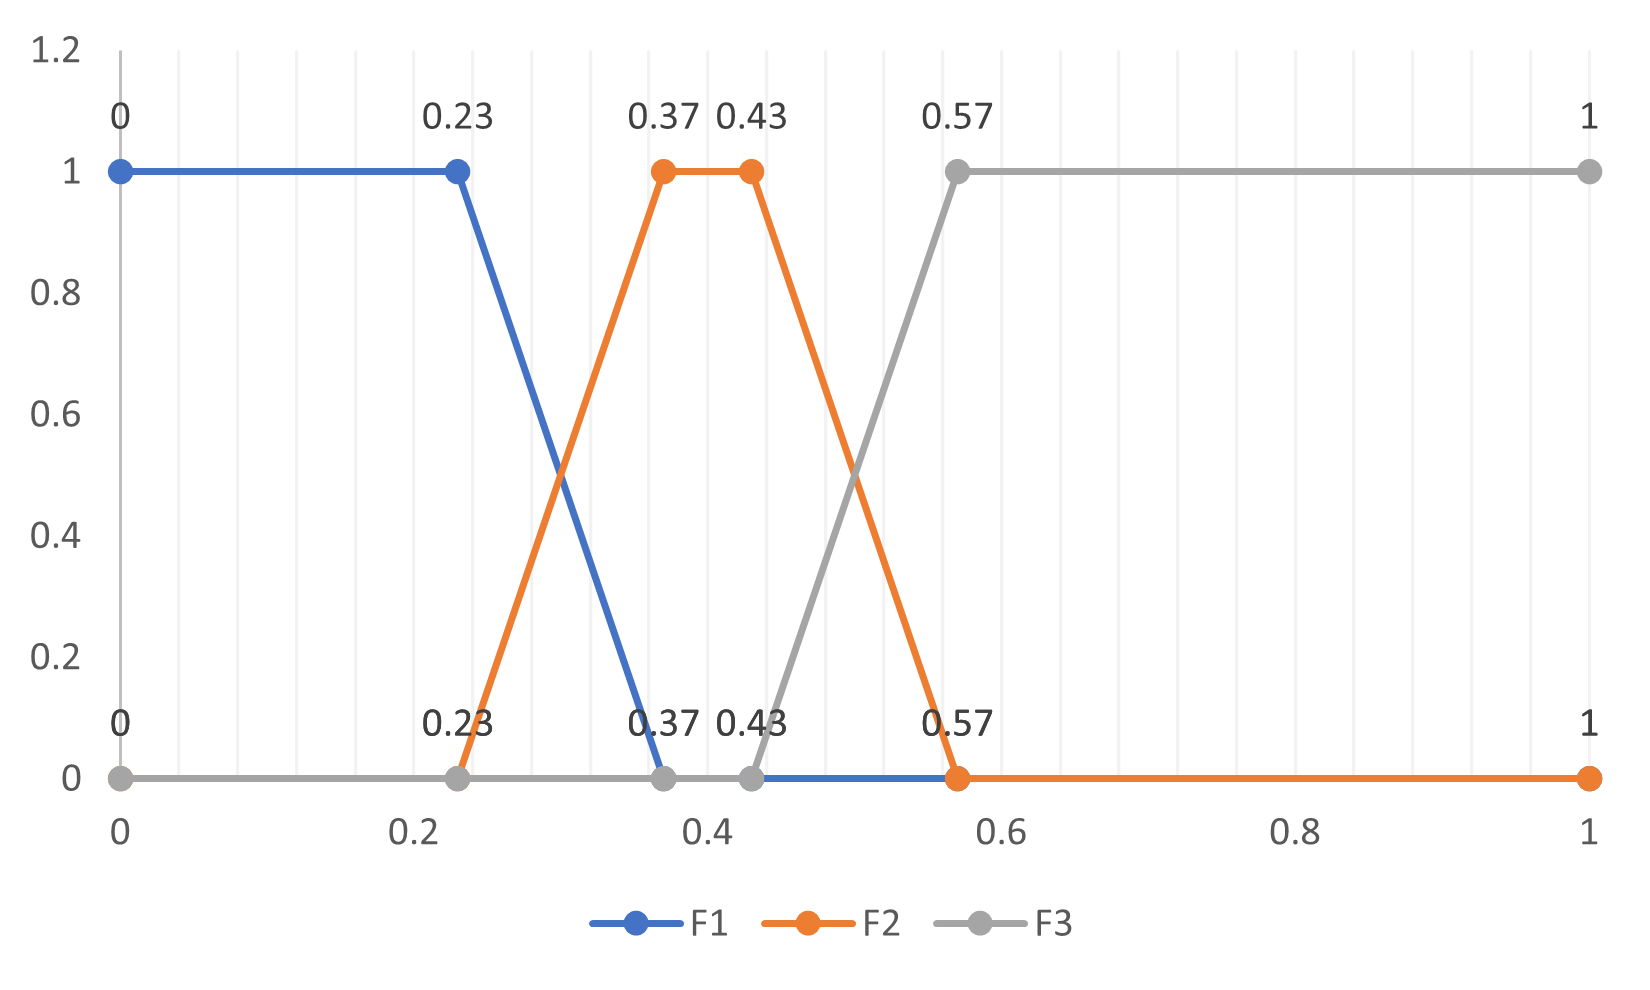
\includegraphics{figs/membership_foodsecurity.png}
      }
      \caption{玉米生产数据模糊隶属函数}
      \label{fig:membership_foodsecurity}
\end{figure}

在确定模糊隶属函数后,按照\ref{chapter:0105}所述的\nameref{alg:FRARAlgorithm}流程,首先构造模糊环境将不同量纲数据归一化到[0,1]区间(在\nameref{subsection:DataCleaning}部分已完成),然后利用\ref{fig:membership_foodsecurity}中的模糊隶属函数将玉米生产数据模糊化,得到三个模糊等价类,然后利用\nameref{def:模糊正域隶属度}计算每个对象对任一条件属性的模糊隶属度,进而由定义\ref{def:模糊依赖度}得到每个条件属性对决策属性的模糊依赖度,最后取该属性的模糊依赖度为其属性重要度,进而得到了每个属性的重要性排名,进而得到该方法下最重要的10个属性。

基于属性重要度的模糊粗糙集属性约简算法作为本文的核心方法,其原理与算法已在\ref{chapter:0105}进行了详尽的阐述。在特征选择过程中以每个省份的粮食生产数据作为一个研究单元,将26个解释变量作为条件属性集,将每亩玉米产量作为决策属性,采用模糊粗糙集属性约简算法进行属性约简,得到每个属性的重要度,计算属性约简耗时,并将每个条件属性的属性重要度作为每个解释变量对玉米产量的影响程度,并按照其属性重要度对属性进行排序,只保留重要性前10的变量作为约简数据集。

% 粗糙集属性约简算法是一种特征选择算法,其基于粗糙集理论,通过删除冗余和不相关的属性,得到一个最小的特征子集,使得该子集可以准确地刻画数据集中的规律和特征,进而达到约简数据集与特征选择的目的。属性约简的目的就是在保证分类准确率的前提下,去除一些无关的条件属性,以减少模型的复杂度和提高模型的泛化能力。\cite{2008Attributes}

% 粗糙集属性约简算法的优点在于具有较好的鲁棒性,能够处理包含不确定性和噪声的数据集,但缺点在于计算复杂度高,且传统的粗糙集属性约简算法只能处理二元属性,无法处理连续属性和模糊属性等不确定性问题。\cite{2020Regional}

% 而基于粗糙集方法的模糊粗糙集属性约简算法作为粗糙集属性约简算法的改进,融合了模糊集合理论和粗糙集理论,能够处理不确定性问题,包括模糊属性和连续属性等,更高的准确性、可靠性及更广泛的应用场景,不仅局限于粗糙集属性约简算法的预测与回归问题。\cite{模糊粗糙集理论研究进展}因在本文实验中需要计算出每个特征的重要性,因此选择基于属性重要度的模糊粗糙集属性约简算法作为研究算法。


\subsection{基于Lasso的特征选择算法}

Lasso(Least Absolute Shrinkage and Selection Operator)是一种线性回归的正则化方法,它在多元线性回归模型的基础上,通过在损失函数中添加$L_1$正则化项来实现特征选择。因添加了$L_1$正则化项的原因,其可以将一些系数收缩为零,从而使得一些系数为零的特征对预测结果没有贡献,进而达到特征选择的效果。下面将从多元线性回归模型开始介绍Lasso的原理。

\subsubsection{多元线性回归模型}
多元线性回归模型是一种用于建模和预测的统计模型,它建立了自变量(特征)和因变量之间的线性关系。假设有一个目标变量(因变量)$Y$和一组自变量(特征)$X_1, X_2,\cdots, X_p$,多元线性回归模型可以表示为:
$$Y=\beta_{0}+\beta_{1} X_{1}+\beta_{2} X_{2}+\ldots+\beta_{p} X_{p}+\varepsilon.$$
其中,$Y$是目标变量的观测值,$\beta_{0}, \beta_{1}, \beta_{2}, \ldots, \beta_{p}$  是模型的系数,表示自变 量对目标变量的影响,$\varepsilon$是误差项,表示模型无法解释的随机误差。

模型的目标是找到最优的系数  $\beta_{0}, \beta_{1}, \beta_{2}, \ldots, \beta_{p} $,使得模型的预测值与实际观测值之间的残差(误差的平方和)最小化。这通常通过最小二乘法来实现,即最小化残差平方和。

然而,多元线性回归模型存在一个问题,即在面对高维数据或特征共线性时,模型的性能可能下降或不稳定。在这种情况下,正则化方法可以用于改善模型的性能和稳定性。Lasso(Least Absolute Shrinkage and Selection Operator)和岭回归(Ridge Regression)都是常见的正则化方法\cite{基于Lasso的我国股票价格影响因素分析}。

\subsubsection{岭回归}

岭回归是多元线性回归的一种扩展方法,通过引入L2正则化项来控制模型的复杂度。L2正则化项是模型系数的平方和乘以一个正则化参数(α),用于惩罚模型系数的大小。岭回归的目标是通过最小化残差平方和和L2正则化项,获得一个系数较小的模型。岭回归的目标函数可以表示为:
$$\min _{\beta_{0}, \beta} \frac{1}{2 n} \sum_{i=1}^{n}\left(y_{i}-\beta_{0}-\sum_{j=1}^{p} x_{i j} \beta_{j}\right)^{2}+\alpha \sum_{j=1}^{p}(\beta_{j})^2.$$
岭回归的$L_2$正则化项对模型系数进行约束,使得模型系数的取值相对较小,从而减小过拟合的风险。与多元线性回归相比,岭回归倾向于得到一个稳定且较简单的模型,而不会将系数完全缩小为零\cite{基于Lasso的我国股票价格影响因素分析}。

\subsubsection{Lasso}
Lasso和岭回归的区别主要在于正则化项的不同。岭回归使用$L_2$正则化,对所有特征进行缩小,适用于具有多个相关特征的问题;Lasso使用$L_1$正则化,可以实现特征选择和稀疏性,适用于具有少量重要特征的问题。Lasso的目标函数为:
$$L(\beta)=\sum_{i=1}^{n}\left(y_{i}-\beta_{0}-\sum_{j=1}^{p} x_{i j} \beta_{j}\right)^{2}+\lambda \sum_{j=1}^{p}\left|\beta_{j}\right|.$$
其中,$n$是样本数,$p$是特征数,$\beta$ 是 $p$ 维系数向量,$\beta_0$ 是截距,$x_{ij}$ 是第 $i$ 个样本第 $j$ 个特征的取值,$y_i$ 是第 $i$ 个样本的目标变量取值,$\lambda$ 是正则化系数。

在存在共线性时,Lasso可能选择其中一个相关特征,而岭回归会将系数平均分配给相关特征。因此Lasso方法的优点在于能够自动选择对目标变量有显著影响的特征,并将其他不重要的特征的系数缩小为零,从而实现特征选择和模型简化。

在Lasso回归中,优化的目标是在保证拟合精度的同时,尽可能使得特征系数之和最小。而正则化系数$\lambda$控制着特征选择的程度,当 $\lambda$ 较大时,意味着正则化罚项的在目标函数中的权重较大,目标函数在优化过程中会因正则化项惩罚较大而使得大部分系数被压缩至零,只有少量的系数会保留,从而实现特征选择的效果\cite{基于Lasso的我国股票价格影响因素分析}。

在Lasso算法实现中,对于Lasso的正则化参数分别选择$\alpha=[0.001, 0.01, 0.1, 1, 10]$,最大迭代次数为1000000。并选用五折交叉验证对模型进行拟合,并计算模型拟合的耗时,选出最佳的模型估计器,并得到其最佳线性系数,那么不同特征对应的系数就是该特征在Lasso模型中的重要度。最后按照最佳线性系数对特征进行排序,并选取前10位特征作为约简数据集。

\subsection{基于随机森林变量重要性的特征选择算法}
随机森林是一种集成学习方法,它由多个决策树组成。每个决策树都是基于不同的随机样本和随机特征训练得到的。在随机森林训练过程中,每个特征都会被分配一个重要性分数,这个分数衡量了该特征对模型预测性能的贡献程度。而特征重要性分数一般有两种计算方法:信息增益和基尼系数。信息增益使用熵和条件熵来计算特征对模型的贡献,基尼系数通过计算特征在样本中出现的概率分布来评估其对模型的影响。在这两种方法中,特征重要性分数越高说明该特征对模型的贡献越大。

基于随机森林变量重要性的特征选择算法通过计算每个特征在随机森林中的重要性分数,按照特征重要性分数从大到小的顺序,逐步选择特征,直到达到预先设定的特征数或特征重要性分数的阈值为止,最终得到的特征集包含对预测结果最有影响的特征。这种方法相对于其他特征选择方法的优点在于其可以同时考虑多个特征之间的互相影响,避免了因单独分析某个特征而忽略了全局其余特征的问题。同时模型具有较好的鲁棒性和泛化能力,可以有效避免模型过拟合问题。
\subsubsection{随机森林模型原理}

随机采样:随机森林的第一步是从原始训练数据集中进行随机采样,构建多个训练子集。采样是有放回地进行的,意味着同一个样本可以在多个子集中出现。通过随机采样,每个训练子集都会略有差异,使得每个子集都具有随机性。这种随机性能够减小模型对训练数据集中的噪声和过拟合的敏感度。

随机特征选择:在随机森林的每个决策树节点进行分裂时,不是使用所有特征,而是随机选择一个特征子集。这样可以减少特征间的相关性,增加模型的多样性。常用的特征选择方法是随机选择$m$个特征,其中$m$是总特征数的平方根或者对数值(取整数部分)。随机特征选择使得每个决策树都只考虑部分特征,增加了模型的多样性。

决策树的构建:对于每个子集和每棵决策树,使用常规的决策树算法(如ID3、CART等)来构建决策树模型。决策树的构建过程中,通过节点的分裂,将样本划分为不同的类别或者进行回归预测。节点的分裂依据是特征的选择,该选择在随机特征选择阶段已经确定。决策树的构建过程会递归进行,直到达到停止条件(如达到最大深度、节点中的样本数小于阈值等)。

预测与集成:在随机森林中,回归问题的预测结果是所有决策树的预测值的平均值。而对于分类问题,采用投票的方式,选择预测结果最多的类别作为最终预测结果。这种集成方式能够平衡不同决策树的预测结果,提高了模型的鲁棒性和准确性。预测与集成过程是随机森林模型的最后一步,通过汇总多个决策树的预测结果来获得最终的预测值或分类结果\cite{随机森林算法优化研究}。
\subsubsection{随机森林变量重要性计算方法}

随机森林通过测量变量在模型中的使用频率和节点分裂时的效果来评估变量的重要性。常用的计算方法有信息增益和基尼系数。

信息增益:随机森林中的每个决策树都可以计算节点分裂时的信息增益,衡量了该特征对于样本分类的贡献程度。通过计算每个特征在所有决策树中的平均信息增益,得到变量的重要性。信息增益越大,说明该特征在随机森林中的重要性越高。

基尼系数:基尼系数是另一种衡量节点分裂的指标,表示了样本被错误分类的概率。计算方式类似于信息增益,通过计算每个特征在所有决策树中的平均基尼系数来评估变量的重要性。基尼系数越小,说明该特征在随机森林中的重要性越高。

通过计算每个特征在所有决策树中的平均信息增益或基尼系数,可以得到变量重要性的排序。较高的变量重要性意味着该特征对模型的预测性能具有更大的贡献\cite{随机森林算法优化研究}。

在随机森林变量重要性算法实现上,设置决策数数量为100,随机种子为42,采用随机森林回归器对玉米生产数据进行训练,得到最佳的随机森林模型,并采用基尼系数计算最佳模型的变量重要性,并按照变量重要性对特征进行排序,得到重要性前10的特征作为约简属性。

\section{对粮食生产数据进行属性约简}
\begin{figure}[htbp]
      \centering
      \resizebox{\textwidth}{!}
      {
      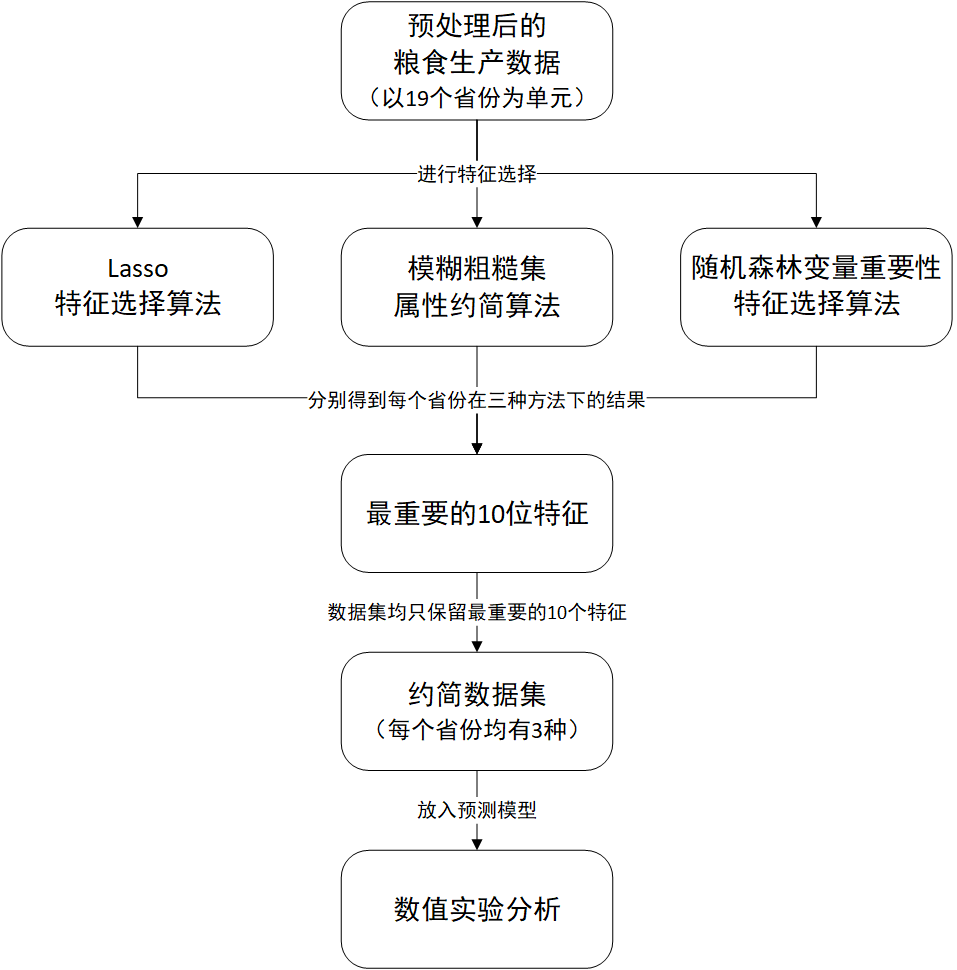
\includegraphics{FeatureSelection}
      }
      \caption{特征选择流程图}
      \label{fig:FeatureSelectionTime}
    \end{figure}
    在特征选择中,分别选择模糊粗糙集属性约简算法(Fuzzy Rough Set Attribute Reduction,以下简记FRAR)、Lasso特征选择算法(Least Absolute Shrinkage and Selection Operator,以下简记Lasso)、随机森林变量重要性特征选择算法(Random Forest,以下简记RF)作为特征选择研究方法,以全国19个省份中每个省份2004-2021年共计26个特征数据为研究对象分别进行特征选择,分别选出每个省份在三种不同方法下最重要的10个特征,并分别计算不同方法的算法耗时。然后对数据集进行属性约简,约简数据集仅保留不同方法下最重要的10位特征,其中每个省份有三份数据集,分别为三种特征选择方法下的约简数据集,之后再对数据集进行数值实验。整体流程图见\ref{fig:FeatureSelectionTime}。
% \begin{algorithm}[htbp]
%       \caption{特征选择算法} %算法的名字
%       \label{alg:FeatureSelectionAlgorithm}
%       \hspace*{0.02in} {\bf 输入:} %算法的输入, \hspace*{0.02in}用来控制位置,同时利用 \\ 进行换行
%       各个省份预处理后的数据AllData\\
%       \hspace*{0.02in} {\bf 输出:} %算法的结果输出
%       各个省份约简后的数据集ReducedData, 特征选择结果ReducedFeatures, 特征选择耗时RunningTime
%       \begin{algorithmic}
%       \For{循环每个省份的数据Data} % For 语句,需要和EndFor对应
%           \State 将Data拆分为特征矩阵X与被解释变量y
%           \State 分别用三种方法进行特征选择
%             \If{FRAR} % If 语句,需要和EndIf对应
%                 \State 计算程序耗时
%                 \State 创建迭代特征的索引     
%                 \State 计算任意两个属性之间的依赖度dep
%                 \State 计算每个属性的不确定度ind
%                 \State 计算每个属性的相对重要度importance=dep-ind
%                 \State 对所有属性按照相对重要度进行排序
%             \ElsIf{Lasso}
%                 \State 选择正则化参数$\alpha$为0.001,0.01,0.1,1,10
%                 \State 最大迭代次数为1000000
%                 \State 交叉验证策略设置为cv=5
%                 \State 计算程序耗时
%                 \State 采用5折交叉验证对Lasso模型进行拟合
%                 \State 选出最佳模型的估计器BestModel与其最佳线性系数coefs
%                 \State 按照最佳线性系数对特征进行排序
%             \ElsIf{RF}
%                 \State 创建随机森林回归器RandomForestRegressor
%                 \State 决策树数量nEstimators设置为100,随机种子为42
%                 \State 计算程序耗时
%                 \State 用随机森林回归器进行训练
%                 \State 提取最佳随机森林模型的特征重要性
%                 \State 按照特征重要性进行排序
%             \EndIf
%           \State 选出排在前10的特征得到特征选择结果ReducedFeatures
%           \State 将原数据集删去未排在重要性前10的特征得到约简数据集ReducedData
%           \State 得到每个省份不同特征选择方法的特征选择耗时RunningTime
%       \EndFor\\
%       \Return 每个省份的约简数据集、特征选择结果及特征选择耗时
%       \end{algorithmic}
%       \end{algorithm}

% 其中,三种特征选择方法进行特征选择的算法实现过程见\nameref{alg:FeatureSelectionAlgorithm},在这里用一层循环实现,循环遍历每个省份的数据,输入数据为excel表格,其中每个sheet存放由\ref{subsection:DataCleaning}进行预处理后的一个省份自2004-2021年的26个解释变量数据。

% 在特征选择方法的算法流程中,模型选择了最常用的参数。对于粗糙集方法选择了基于属性重要度的模糊粗糙集属性约简算法,利用列表推导式分别算出任意两个属性之间的依赖度与每个属性的不确定度,再将依赖度减去不确定度计算出每个属性的相对重要度,最后根据相对重要度对属性进行排序。对于Lasso方法,正则化参数$\alpha$为0.001、0.01、0.1、1、10,最大迭代次数设置为1000000,并采用5折交叉验证进行拟合,得到最佳模型,并导出最佳模型中每个特征的线性系数,再根据线性系数进行排序。对于随机森林模型,决策树数量设置为100,随机种子设置为42,创建随机森林回归器并训练得到最佳模型,提取出最佳模型的特征重要性,再按照特征重要性进行排序。最后得到每个省份在不同特征选择方法下的特征选择结果、特征选择耗时与约简数据集。
\section{特征选择结果}
本节将展示对三种不同特征选择方法的特征选择结果,包括特征选择后的特征与算法耗时,约简数据集将在\ref{chapter:3}中进行数值实验。
\subsection{属性约简后的结果}
每个省份的数据集经过特征选择后,分别得到了不同方法下最重要的10个特征,结果见\ref{table:Feature5_FRAR}(在此仅展示FRAR的前5位特征,其余见附录),并据此数据集进行属性约简,得到各省份在不同方法下的约简数据集,以便后续进行数值实验分析。
\begin{table}[htbp]
      \centering
      \caption{FRAR:各省份前5位特征}
      \label{table:Feature5_FRAR}
      \resizebox{\textwidth}{!}
      {
      \csvautobooktabular{data/ReducedFeatures_FRAR.csv}
      }
\end{table}

\subsection{算法耗时比较}

% 将csv文件载入数据库
\DTLloaddb{RunningTime}{data/RunningTime.csv}
\begin{table}[htbp]
      \centering
      \caption{特征选择算法耗时比较(单位:秒)}
      \label{table:RunningTime}
      \csvautobooktabular{data/RunningTime.csv}
\end{table}

在特征选择过程中,分别计算了各省份在不同算法下的特征选择耗时,其中对三种方法的计时标准进行了统一,计时部分均只有三种特征选择方法的函数调用主体,三个函数输入均为各省的玉米生产数据,输出均为所有变量的重要性,通过统一函数的输入与输出来比较不同算法的耗时。结果如\ref{table:RunningTime}所示。可以看到,Lasso平均耗时大致为随机森林变量重要性方法RF平均耗时的两到三倍,模糊粗糙集属性约简算法FRAR的平均耗时为Lasso的一半,为RF的1.5倍,FRAR方法的耗时较Lasso快,稍慢于RF。

这也说明了模糊粗糙集属性约简算法相较于基于回归方法的Lasso不需要大量的交叉验证进行拟合优化,因而算法效率较Lasso高。而与RF相比,FRAR算法多出的耗时相较于Lasso能够忍受,其耗时大部分花费在对数据进行模糊化过程中的计算模糊隶属度方面,如果能在这方面对代码进行进一步的优化,则其算法效率还可进一步提高。




%%%%%%%%%%%%%%%%%%%%%%%%%%%%%%%%%%%%%%%%%%%%%%%%%%%%%%%%%%%%%%%%%%%%%
% \section{学习资源}

% 对于数学公式的排版在\enquote{lshort-zh-cn.pdf}的第四章给出了基本的使用方法,
% 请大家阅读学习。其内容对大多数人来说已经足够用了,但是如果不能解决问题的话
% 建议大家求助于搜索引擎或者有经验的人,这也不失为一个好办法。

% 常见的几个学习\LaTeX{}数学公式排版的资源链接如下:

% \begin{itemize}
%   \item 数学排版常见问题集:
%         \url{https://www.latexstudio.net/index/details/index/mid/635}
%   \item \pkg{amsmath}手册中译:
%         \url{https://www.latexstudio.net/index/details/index/mid/706}
%   \item \LaTeX{}公式备忘单:
%         \url{https://www.latexstudio.net/index/details/index/mid/1052.html}
% \end{itemize}

% \section{公式排版与注解}

% 按我校学位论文排版要求,公式排版需要行间居中排版,公式编号按照一级标题(章)
% 连续编号(按章)并加小括号,不加导引线。类似这些细节\nwafuthesis{}模板都已进
% 行了设置。在撰写论文中只要将公式置于\env{equation}环境,并用\cs{label}命令
% 添加标签后用\cs{ref}或\cs{eqref}命令引用该公式即可。对于多行公式可以在
% \env{equation}环境中使用\env{aligned}环境实现排版。

% 需要注意的是,公式解释下面的\enquote{式中}两字需要左起顶格编排,后接符号及
% 其解释;解释顺序为先左后右,先上后下;解释与解释之间用中文分号“;”分隔。
% 此时可以用\cs{noindent}命令临时取消首行缩进,在解释完公式符号后,再次正常
% 用空行进行分段便可自动恢复段落首行缩进。

% 例如:勾股定理可以表示为\ref{eq:gougu}

% \begin{equation}
%   a^2+b^2=c^2\label{eq:gougu}
% \end{equation}

% \noindent
% 式中,$a$是一条直角边边长;$b$是另一条直角边边长;$c$是斜边边长。

% 在公式解释结束后,段落缩进应复位至首行缩进2个汉字的模式。

% \section{模板提供的数学环境}

% \nwafuthesis{} 提供了一系列预定义的数学环境,详情见\nwafuthesis{}说明书的表6。
% 其使用样例有以下7种形式。

% \subsection{axiom公理环境}

% \begin{axiom}[欧几里得距离]
% 点$\mathbf{p}$与点$\mathbf{q}$的\textbf{欧几里德距离},是连接两点的线段
% ($\overline{\mathbf{pq}}$)的长度。

% 在笛卡尔坐标系下,如果 $n$维欧几里得空间下的两个点 $\mathbf{p}=(p_1, p_2,
% \dots, p_n)$ 与点$\mathbf{q} = (q_1, q_2, q_3, \dots, q_n)$,那么点$\mathbf{p}$
% 与点$\mathbf{q}$的距离,或者点$\mathbf{q}$与点$\mathbf{p}$的距离,由
% \autoref{equ:1}定义:
% \begin{align}
% d(\mathbf{p},\mathbf{q}) = d(\mathbf{q},\mathbf{p}) & = \sqrt{(q_1-p_1)^2
%                          + (q_2-p_2)^2 + \cdots + (q_n-p_n)^2} \notag \\
% \label{equ:1}
% & = \sqrt{\sum_{i=1}^n (q_i-p_i)^2}
% \end{align}
% \end{axiom}

% \subsection{corollary推论环境}

% \begin{corollary}[欧几里得距离]
% 点$\mathbf{p}$与点$\mathbf{q}$的\textbf{欧几里德距离},是连接两点的线段
% ($\overline{\mathbf{pq}}$)的长度。

% 在笛卡尔坐标系下,如果 $n$维欧几里得空间下的两个点 $\mathbf{p}=(p_1, p_2,
% \dots, p_n)$ 与点$\mathbf{q} = (q_1, q_2, q_3, \dots, q_n)$,那么点$\mathbf{p}$
% 与点$\mathbf{q}$的距离,或者点$\mathbf{q}$与点$\mathbf{p}$的距离,由
% \autoref{equ:2}定义:
% \begin{align}
% d(\mathbf{p},\mathbf{q}) = d(\mathbf{q},\mathbf{p}) & = \sqrt{(q_1-p_1)^2
%                          + (q_2-p_2)^2 + \cdots + (q_n-p_n)^2} \notag \\
% \label{equ:2}
% & = \sqrt{\sum_{i=1}^n (q_i-p_i)^2}
% \end{align}
% \end{corollary}

% \subsection{definition定义环境}

% \begin{definition}[欧几里得距离]
% 点$\mathbf{p}$与点$\mathbf{q}$的\textbf{欧几里德距离},是连接两点的线段
% ($\overline{\mathbf{pq}}$)的长度。

% 在笛卡尔坐标系下,如果 $n$维欧几里得空间下的两个点 $\mathbf{p}=(p_1, p_2,
% \dots, p_n)$ 与点$\mathbf{q} = (q_1, q_2, q_3, \dots, q_n)$,那么点$\mathbf{p}$
% 与点$\mathbf{q}$的距离,或者点$\mathbf{q}$与点$\mathbf{p}$的距离,由
% \autoref{equ:3}定义:
% \begin{align}
% d(\mathbf{p},\mathbf{q}) = d(\mathbf{q},\mathbf{p}) & = \sqrt{(q_1-p_1)^2
%                          + (q_2-p_2)^2 + \cdots + (q_n-p_n)^2} \notag \\
% \label{equ:3}
% & = \sqrt{\sum_{i=1}^n (q_i-p_i)^2}
% \end{align}
% \end{definition}

% \subsection{example示例环境}

% \begin{example}[欧几里得距离]
% 点$\mathbf{p}$与点$\mathbf{q}$的\textbf{欧几里德距离},是连接两点的线段
% ($\overline{\mathbf{pq}}$)的长度。

% 在笛卡尔坐标系下,如果 $n$维欧几里得空间下的两个点 $\mathbf{p}=(p_1, p_2,
% \dots, p_n)$ 与点$\mathbf{q} = (q_1, q_2, q_3, \dots, q_n)$,那么点$\mathbf{p}$
% 与点$\mathbf{q}$的距离,或者点$\mathbf{q}$与点$\mathbf{p}$的距离,由
% \autoref{equ:4}定义:
% \begin{align}
% d(\mathbf{p},\mathbf{q}) = d(\mathbf{q},\mathbf{p}) & = \sqrt{(q_1-p_1)^2
%                          + (q_2-p_2)^2 + \cdots + (q_n-p_n)^2} \notag \\
% \label{equ:4}
% & = \sqrt{\sum_{i=1}^n (q_i-p_i)^2}
% \end{align}
% \end{example}

% \subsection{lemma引理环境}

% \begin{lemma}[欧几里得距离]
% 点$\mathbf{p}$与点$\mathbf{q}$的\textbf{欧几里德距离},是连接两点的线段
% ($\overline{\mathbf{pq}}$)的长度。

% 在笛卡尔坐标系下,如果 $n$维欧几里得空间下的两个点 $\mathbf{p}=(p_1, p_2,
% \dots, p_n)$ 与点$\mathbf{q} = (q_1, q_2, q_3, \dots, q_n)$,那么点$\mathbf{p}$
% 与点$\mathbf{q}$的距离,或者点$\mathbf{q}$与点$\mathbf{p}$的距离,由
% \autoref{equ:5}定义:
% \begin{align}
% d(\mathbf{p},\mathbf{q}) = d(\mathbf{q},\mathbf{p}) & = \sqrt{(q_1-p_1)^2
%                          + (q_2-p_2)^2 + \cdots + (q_n-p_n)^2} \notag \\
% \label{equ:5}
% & = \sqrt{\sum_{i=1}^n (q_i-p_i)^2}
% \end{align}
% \end{lemma}

% \subsection{proof证明环境}

% \begin{proof}[欧几里得距离]
% 点$\mathbf{p}$与点$\mathbf{q}$的\textbf{欧几里德距离},是连接两点的线段
% ($\overline{\mathbf{pq}}$)的长度。

% 在笛卡尔坐标系下,如果 $n$维欧几里得空间下的两个点 $\mathbf{p}=(p_1, p_2,
% \dots, p_n)$ 与点$\mathbf{q} = (q_1, q_2, q_3, \dots, q_n)$,那么点$\mathbf{p}$
% 与点$\mathbf{q}$的距离,或者点$\mathbf{q}$与点$\mathbf{p}$的距离,由
% \autoref{equ:6}定义:
% \begin{align}
% d(\mathbf{p},\mathbf{q}) = d(\mathbf{q},\mathbf{p}) & = \sqrt{(q_1-p_1)^2
%                          + (q_2-p_2)^2 + \cdots + (q_n-p_n)^2} \notag \\
% \label{equ:6}
% & = \sqrt{\sum_{i=1}^n (q_i-p_i)^2}
% \end{align}
% \end{proof}

% 证明与其他定理环境稍有不同, 末尾会有一个 QED 符号。

% \subsection{theorem定理环境}

% \begin{theorem}[欧几里得距离]
% 点$\mathbf{p}$与点$\mathbf{q}$的\textbf{欧几里德距离},是连接两点的线段
% ($\overline{\mathbf{pq}}$)的长度。

% 在笛卡尔坐标系下,如果 $n$维欧几里得空间下的两个点 $\mathbf{p}=(p_1, p_2,
% \dots, p_n)$ 与点$\mathbf{q} = (q_1, q_2, q_3, \dots, q_n)$,那么点$\mathbf{p}$
% 与点$\mathbf{q}$的距离,或者点$\mathbf{q}$与点$\mathbf{p}$的距离,由
% \autoref{equ:7}定义:
% \begin{align}
% d(\mathbf{p},\mathbf{q}) = d(\mathbf{q},\mathbf{p}) & = \sqrt{(q_1-p_1)^2
%                          + (q_2-p_2)^2 + \cdots + (q_n-p_n)^2} \notag \\
% \label{equ:7}
% & = \sqrt{\sum_{i=1}^n (q_i-p_i)^2}
% \end{align}
% \end{theorem}


% \section{交叉引用}

% 与图表一样,公式、定理等也需要采用专用的命令或环境进行排版以实现
% 编号、交叉引用等\emph{自动化}处理,\emph{万万不可}手动编号、引用!


%%% Local Variables: 
%%% mode: latex
%%% TeX-master: "../main.tex"
%%% End:

% 本文件是示例论文的一部分
% 论文的主文件位于上级目录的 `main.tex`
\chapter{利用粮食生产预测模型进行分析与验证}
\label{chapter:4}
本章主要对\ref{chapter:3}中得到的特征选择结果和约简数据集进行数值实验分析,通过将原数据集与约简数据集中2004-2020年的数据投入预测模型进行训练,并预测2021年各省份的产量,再与真实值进行比较,以便通过预测模型结果分析特征选择结果的优劣。
\section{预测模型数值实验}
\begin{figure}[!htb]
  \centering
  \resizebox{\textwidth}{!}
  {
  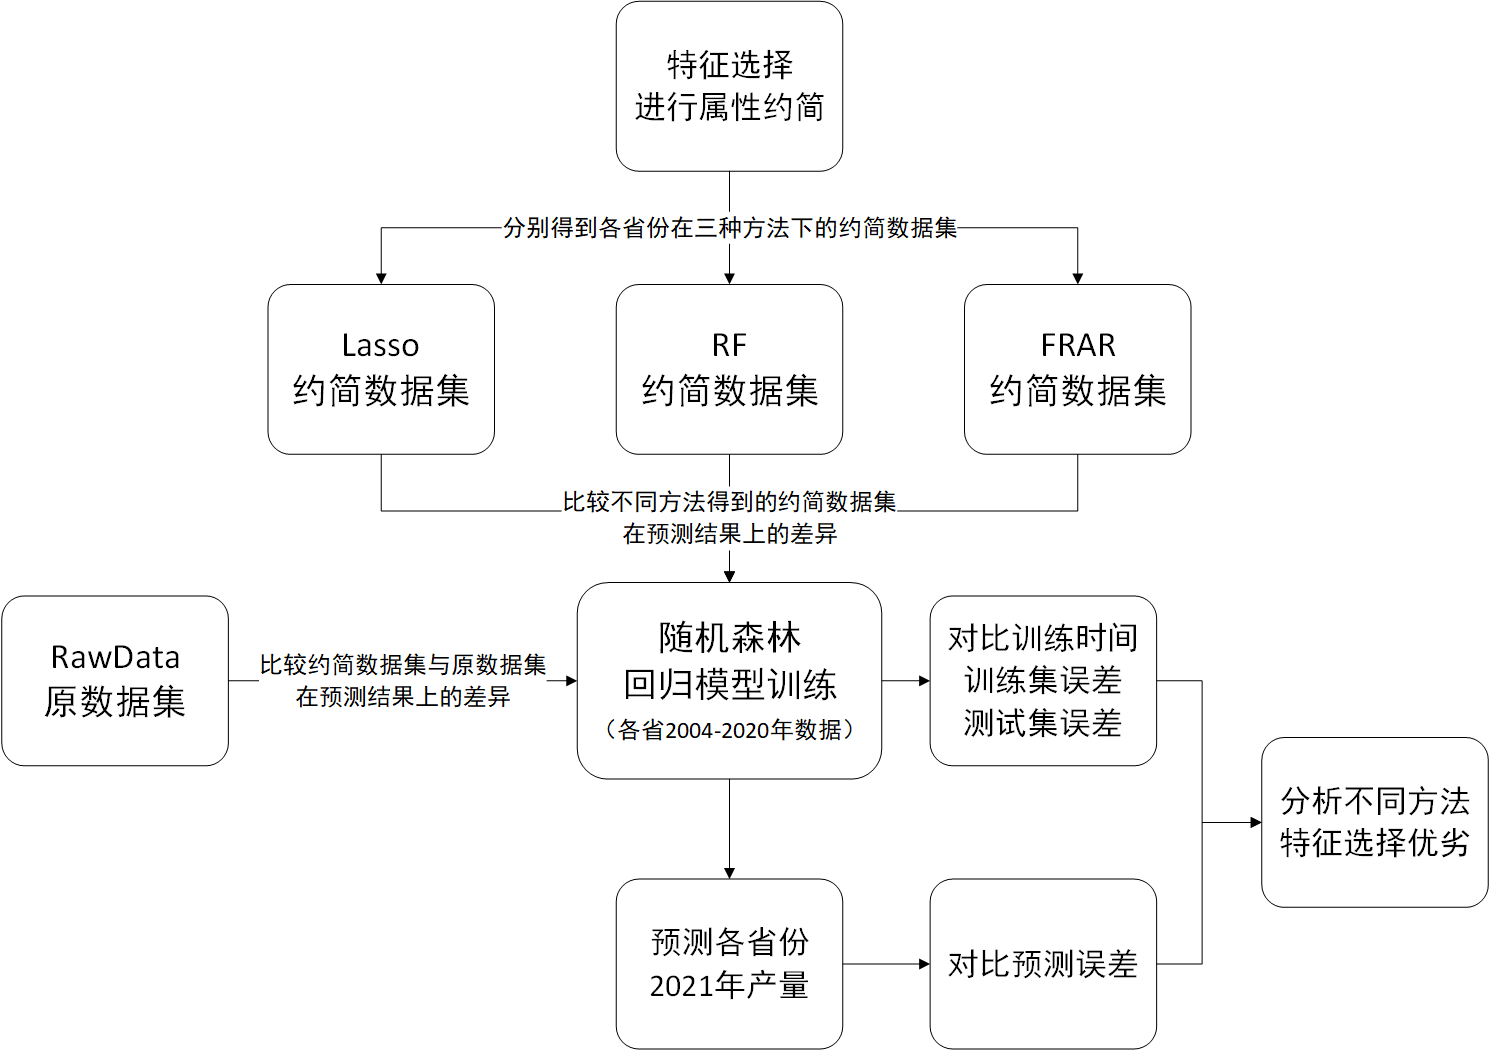
\includegraphics{PredictionVerification}
  }
  \caption{预测模型数值实验流程图}
  \label{fig:PredictionVerification}
\end{figure}

本章预测模型的数值实验主要目标是通过将不同特征选择方法得到的约简数据集放入预测模型,通过预测实验分析得到其模型的拟合效果与泛化能力,进而分析出约简数据集中特征的信息表现能力,以便对三种特征选择方法的特征选择结果进行评价与比较。

对于属性约简的评估方法,针对不同类型数据有着不同的评估方法。对于分类与回归问题,主要有决策树、随机森林、朴素贝叶斯、支持向量机、KNN等方法\cite{BestOverview}。本数值实验选择随机森林回归模型来作为预测模型对数据集进行实验分析。因随机森林变量重要性方法(RF)作为随机森林模型的一部分,其选择出的特征正是随机森林模型中对目标变量贡献最大的,因而将选出的特征放入模型进行试验将具有较优的拟合效果与表现。而随机森林模型自身在预测中本就有着较好的鲁棒性,因而可以将RF方法的实验结果作为一个较优的参考,进而可以据此来评价其余方法在预测模型中的表现,进而分析不同特征选择方法的特征选择效果。

本章数值实验的数据基于\ref{chapter:3}的三种特征选择方法的约简数据集与未约简原数据集,将每省的数据作为一个分析单元,横向对比同一省份不同数据集的预测效果,纵向分析不同省份相同预测模型指标的差异。以每省2004-2020年数据作为数据集,并将数据集按照8:2随机分为训练集与测试集,比较不同数据集在训练时间、训练误差、测试误差方面的差异,进而分析不同数据集在拟合效果方面的不同。然后将各省2021年的数据作为预测变量,预测各省2021年的作物产量,再与真实值比较得出预测误差,分析不同数据集在预测精度方面的优劣,进而得到不同数据集的泛化能力。最后综合比较约简数据集与未约简原数据集在预测模型表现上的差异,分析出在预测前将数据集进行属性约简对预测结果的影响,得到最终的实验分析结果。具体流程见\ref{fig:PredictionVerification}。

% 其中,预测数值实验具体算法流程见\nameref{alg:PredictionAlgorithm},预测模型仍然选为随机森林回归模型,参数设置与\nameref{alg:FeatureSelectionAlgorithm}一致。该算法由两层循环实现,第一层循环遍历所有省份,第二层循环遍历每个省份的四个数据集。在第一层循环中分别取出当前Province在原数据集RawData及及三种不同方法下的约简数据集FRAR、Lasso、RF,并将其合并为一个字典DataDict。然后在第二层循环中分别对字典中的每个数据集应用随机森林回归模型进行拟合,并计算出当前数据集的训练时间TrainTime、训练误差TrainRMSE、测试误差TestRMSE及预测精度PredError,最后再将每个省份在四个不同数据集下的拟合结果保存下来。

% \begin{algorithm}[htbp]
%   \caption{预测模型数值实验算法} %算法的名字
%   \label{alg:PredictionAlgorithm}
%   \hspace*{0.02in} {\bf 输入:} %算法的输入, \hspace*{0.02in}用来控制位置,同时利用 \\ 进行换行
%   所有省份原数据集RawData、三种不同方法下的约简数据集FRARData、LassoData、RFData\\
%   \hspace*{0.02in} {\bf 输出:} %算法的结果输出
%   各个省份在四个不同数据集下的训练时间TrainTime、训练误差TrainRMSE、测试误差TestRMSE及预测精度PredError
%   \begin{algorithmic}
%   \For{循环每个省份Province} % For 语句,需要和EndFor对应
%       \State 分别取出四个数据集中Province省份的数据:RawData、FRAR、Lasso、RF,将其合并为一个字典DataDict
%       \For{循环对字典DataDict中的每个数据集Data进行预测} 
%             \State 将Data拆分为特征矩阵X与被解释变量y
%             \State 按照8:2的比例将数据集随机拆分为训练集与测试集,随机种子为42
%             \State 开始计算训练耗时
%             \State 创建随机森林回归器RandomForestRegressor
%             \State 决策树数量nEstimators设置为100,随机种子为42
%             \State 用随机森林回归器对训练集进行训练
%             \State 结束计算训练耗时并计算训练耗时TrainTime
%             \State 计算训练集均方误差TrainRMSE
%             \State 将测试集放入模型进行测试并计算测试集均方误差TestRMSE
%             \State 预测2021年的玉米产量yPred2021
%             \State 根据2021年真实值与预测值计算二者的偏差PredError
%         \EndFor
%       \State 保存Province在四个数据集下的TrainTime、TrainRMSE、TestRMSE、PredError
%   \EndFor\\
%   \Return 每个省份在四个数据集下的TrainTime、TrainRMSE、TestRMSE、PredError
%   \end{algorithmic}
%   \end{algorithm}

\section{三种特征选择方法的数值实验比较}
本节主要将各省份由三种特征选择方法(Lasso,RF,FRAR)得到的约简数据集与未约简原数据集放入预测模型中进行预测实验,通过比较不同数据集在训练时间、训练集误差、测试集误差、预测值误差方面的差异,以便通过预测结果表现来评价不同特征选择算法在特征选择上的优劣。

\subsection{耗时比较}
在随机森林预测模型训练过程中,计算了各省不同数据集的训练耗时。训练耗时在某种程度上意味着预测模型在训练过程中的学习成本,训练耗时越久,意味着模型在学习数据集特征上的成本越大,数据集所提供的信息越不明显,需要更多次的优化与训练才能学习到足够的信息。其中训练耗时的计算范围为调用sklearn.ensemble库中的RandomForestRegressor函数建立随机森林回归模型,然后利用该模型对已经划分好的训练数据集进行拟合,以此来计算各个数据集在拟合随机森林模型过程的耗时。具体结果见\ref{table:Pred_train_time},从表格中结果可以看出:
\begin{enumerate}
\item 三种约简数据集相较于原数据集在训练时间上确实有所减少,但减少效果上并不是非常显著。
\item RF和FRAR约简数据集在平均训练耗时上较原数据集约快5\% ,Lasso约简数据集平均较原数据集快1\%。
\item Lasso约简数据集对训练耗时基本无提高,FRAR与RF约简数据集在训练耗时方面有一定提高,但不明显。
\end{enumerate}
\DTLloaddb{Pred_train_time}{data/Pred_train_time.csv}
\begin{table}[htbp]
      \centering
      \caption{训练耗时(单位:秒)}
      \label{table:Pred_train_time}
      \csvautobooktabular{data/Pred_train_time.csv}
\end{table}
\subsection{误差比较}
在划分数据集过程中,使用随机数种子42按照8:2的比例将数据分为训练集与测试集。分别计算各省份在不同方法下的训练集均方误差和测试集均方误差,并比较不同数据集在均方误差上的差异。具体训练集均方误差见\ref{table:Pred_train_rmse},测试集均方误差见\ref{table:Pred_test_rmse}。从表格中结果可以得出:
\DTLloaddb{Pred_train_rmse}{data/Pred_train_rmse.csv}
% \begin{table}
%       \centering
%       \caption{训练集误差}
%       \label{table:Pred_train_rmse}
%       \csvautobooktabular{data/Pred_train_rmse.csv}
% \end{table}
\DTLloaddb{Pred_test_rmse}{data/Pred_test_rmse.csv}
% \begin{table}
%       \centering
%       \caption{测试集误差}
%       \label{table:Pred_test_rmse}
%       \csvautobooktabular{data/Pred_test_rmse.csv}
% \end{table}
% \begin{figure}[htbp]
%   \centering
%   \begin{minipage}[t]{0.5\linewidth}
%     \centering
%     \resizebox{\textwidth}{!}
%     {
%     \csvautobooktabular{data/Pred_train_rmse.csv}
%     }
%     \caption{表格 1}
%     \label{fig:table1}
%   \end{minipage}%
%   \begin{minipage}[t]{0.5\linewidth}
%     \centering
%     \resizebox{\textwidth}{!}
%     {
%     \csvautobooktabular{data/Pred_test_rmse.csv}
%     }
%     \caption{表格 2}
%     \label{fig:table2}
%   \end{minipage}
% \end{figure}
\begin{figure*}[htbp]
  \centering
  \subfloat[训练集误差\label{table:Pred_train_rmse}]{
    \resizebox{0.5\textwidth}{!}
    {
    \csvautobooktabular{data/Pred_train_rmse.csv}
    }
  }
  \subfloat[测试集误差\label{table:Pred_test_rmse}]
  {
    \resizebox{0.5\textwidth}{!}
    {
    \csvautobooktabular{data/Pred_test_rmse.csv}
    }
  }
  \caption{数据集均方误差}
  \label{table:Pred_rmse}
\end{figure*}
\begin{enumerate}
  \item RF和FRAR在训练集误差与测试集误差方面均显著优于原数据集,均方误差较原数据集减少了约15\%,而且FRAR在均方误差上非常接近RF,略微大于RF,在拟合效果与泛化能力方面有着与RF接近的表现。
  \item Lasso在训练集误差与测试集误差方面与原数据集基本无较大差异,均方误差减少不到5\%。对于误差的减少程度非常有限,几乎可忽略不计,在拟合效果与泛化能力方面并无显著改进。
  \item 三种方法的约简数据集在模型拟合效果与泛化误差方面确实较原数据集有改进与提高,但Lasso约简数据集的改进效果并不明显。而RF与FRAR的效果较为显著,且FRAR在均方误差上与RF非常接近。
  \end{enumerate}
\subsection{预测精度比较}
每个省份在模型训练结束后,分别对不同数据集预测了2021年的作物产量,并与2021年的作物产量真实值进行了比较,计算了每个省份不同约简数据集的预测相对误差,其中预测相对误差计算公式为:$$\text{预测相对误差}=\frac{\left|\text{预测值}-\text{真实值}\right|}{\text{真实值}}$$
具体预测相对误差见\ref{table:Pred_pred_error}。从表格中结果可以得出:
\begin{enumerate}
  \item Lasso约简数据集在预测精度上相对于原数据集不升反降,在大多数省份中的预测效果不如原数据集精确,预测效果不佳。
  \item RF与FRAR的预测精度相较原数据集有非常大的提高,RF约简数据集预测误差较原数据集减少了约25\%,而FRAR约简数据集预测误差较原数据集减少了20\%。
  \item 预测相对误差代表着模型的泛化能力及预测精度,综合结果看出RF约简数据集的预测效果最佳,FRAR约简数据集预测效果略微低于RF,精度与RF非常接近,Lasso预测效果不升反降。
\end{enumerate}
\DTLloaddb{Pred_pred_error}{data/Pred_pred_error.csv}
\begin{table}[htbp]
      \centering
      \caption{预测相对误差}
      \label{table:Pred_pred_error}
      \csvautobooktabular{data/Pred_pred_error.csv}
\end{table}
\section{数值实验结果分析}
本节主要对不同特征选择方法的数值实验结果进行分析,总结不同特征选择方法的优劣。
\subsection{Lasso}
基于Lasso的特征选择算法是一种较为经典的特征选择算法,经过上节实验分析可以看出,Lasso方法综合在各方面的表现都不如其余方法,具体分析如下:
\begin{enumerate}
  \item 在特征选择时间上,Lasso方法在耗时上最长,特征选择时间最久,算法复杂度最高,所耗费的时间成本最大,高于其余方法。
  \item 在训练耗时上,经过该方法约简后的数据集与原数据集并无较大提高,与其余两种方法有着较大差距,说明其在本文实验中并未明显达到属性约简后简化模型节约训练时间的目的。
  \item 在模型拟合效果上,Lasso数据集的训练集误差与测试集误差较原数据集提高非常有限,基本与原数据集持平,说明在本文实验中经过该方法进行属性约简后的数据集并没有能更好的拟合预测模型,没有达到提高泛化能力的目标。
  \item 在预测精度上,Lasso数据集的预测精度较原数据集不增反降,说明在本文实验中经过Lasso方法进行属性约简后数据集的并不能很好的用于预测,特征选择没有达到提高表现的目标。
  \item 在特征选择能力上,经过Lasso方法约简后的数据集在预测模型中并没有达到其避免过拟合且提高泛化能力的目标,说明在本实验中Lasso方法没有真正起到特征选择的作用,没有选出真正重要的因素,特征选择效果并不佳。
\end{enumerate}
\subsection{RF}
基于随机森林变量重要性的特征选择算法作为本预测模型——随机森林模型的一部分,其数值实验结果理论上应有着最优的表现,具体分析如下:
\begin{enumerate}
  \item 在特征选择时间上,RF方法耗时较Lasso方法快了约三倍,算法复杂度比Lasso方法低,时间成本更低。
  \item 在训练耗时上RF数据集也有着最优的表现,虽平均耗时最短,但未有着非常明显的提升,仅较原数据集提高约5\%,可能与数据集较小使得耗时差异并不明显有关。
  \item 在模型拟合效果上,RF数据集的训练集误差与测试集误差也均为最优,发挥了其作为参考模型的作用,说明在本文实验中RF在特征选择上达到了提高泛化能力及拟合效果最优的目标。
  \item 在预测精度上,RF数据集同样有着最优的表现。说明在本文实验中RF特征选择处理对提高预测模型的预测精度有着较大帮助,并且泛化能力最佳。
  \item 在特征选择能力上,经过RF方法约简的数据集在各方面都有着最优的表现,这与理论上随机森林模型自身选出的最重要的特征对自己预测模型的拟合效果表现较优相符。说明RF方法确实起到了特征选择的作用,且效果最佳,可以将其作为其它方法表现优劣的一个参考,选出的因素有着一定的参考价值。但考虑到预测模型也为随机森林模型,不能确定随机森林变量重要性方法在其余预测模型上也能表现较优,只能在此模型中作为一个衡量Lasso方法与FRAR方法表现的标杆。
\end{enumerate}
\subsection{FRAR}
FRAR方法是本文的核心方法,在数值实验的预测模型中选择随机森林模型,RF约简数据集对于随机森林预测模型拟合最优,可以将RF约简数据集结果作为一个参考,通过比较FRAR数据集与RF数据集的差距,可以衡量其在各方面的表现,具体分析如下:
\begin{enumerate}
  \item 在特征选择时间上,FRAR方法较Lasso提高了一倍,但略慢于RF方法。这也说明基于属性重要度的模糊粗糙集属性约简算法在算法复杂度方面较基于线性回归的Lasso不需要进行复杂的交叉验证拟合,算法绝大部分将时间花费在连续属性模糊化过程中,其余均为取大取小运算,如果能对模糊化部分代码进行优化,还能有着进一步的提高。
  \item 在训练耗时上,FRAR数据集较原数据集有较大提升,仅次于RF数据集,且与RF数据集非常接近,说明在本文实验中FRAR算法能够很好的简化模型并节约训练时间。
  \item 在模型拟合效果上,FRAR数据集的训练集误差与测试集误差均表现较好,且与拟合最优的RF数据集表现极为接近。说明在本文实验中FRAR数据集能够很好的拟合预测模型并具有很强的泛化能力,可以达到与RF相近的表现。
  \item 在预测精度上,FRAR数据集较原数据集减少了20\%的预测相对误差,且较拟合最优的RF数据集在预测相对误差方面仅高了0.002,预测精度有着较优的表现。说明在本文实验中FRAR数据集有着较为出色的泛化能力,且能够准确地用于预测。
  \item 在特征选择能力上,经预测模型数值实验结果可以看出,FRAR方法无论在耗时还是拟合效果上都仅次于RF方法,且均与表现最佳的RF方法非常接近。说明经过FRAR约简后的数据集能够保留最重要的特征,并且达到简化模型提高拟合效果的目的。进而说明在本文实验中FRAR的特征选择效果较优,能够选出重要的特征,且算法复杂度较低。
\end{enumerate}
\subsection{结论}
综合数值实验结果与分析,可以得到如下结论:
\begin{enumerate}
  \item 基于属性重要度的模糊粗糙集属性约简算法(FRAR)在特征选择耗时、效果及约简数据集在预测模型的误差、耗时等方面都仅次于RF方法,且与表现最优的RF方法非常接近,说明模糊粗糙集属性约简算法在特征选择方面有着较大的优势。
  \item 基于Lasso的特征选择算法在各方面表现不佳,与FRAR算法在各方面有着较大的差距。基于随机森林变量重要性的特征选择算法(RF)在各方面表现均最佳,这与理论上随机森林模型自身选出的变量对自己的拟合最优相应,说明其可以作为检验其余两种方法表现的标杆。但本文实验结果也仅展示了其在自身预测模型上的表现,其作为特征选择方法在其他预测模型上的效果表现是否仍会保持最优的效果还有待进一步实验验证,这部分内容就不在本文的讨论范围内了。
  \item 经数值实验验证分析可得,基于属性重要度的模糊粗糙集属性约简算法在特征选择结果上得出的影响各省作物产量的最重要10位因素可以较充分的解释因变量的变化,可以选择其结果做进一步的粮食安全分析。
\end{enumerate}

%%%%%%%%%%%%%%%%%%%%%%%%%%%%%%%%%%%%%%%%%%%%%%%%%%%%%5555



% \section{正文中参考文献的引用}

% 为了规范我校学位论文写作,我校学位论文的参考文献采用采用
% \enquote{著者-出版年}制进行文献的引用与著录。
% \subsection{著者作为引用主语}
% 文中提及著者,在被引用的著者姓名或外国著者姓氏之后用圆括号标注文献出版年,
% 可使用\cs{textcite}、\cs{yearcite}命令或手动模式引用文献,如:

% \begin{center}
%   \begin{minipage}{0.45\textwidth}
%     \small
%     \verb|\textcite{赵耀东1998--}|指出...

%     赵耀东\verb|\yearcite{赵耀东1998--}|指出...

%     赵耀东\verb|(\cite*{赵耀东1998--})|指出...

%     赵耀东\verb|(\citeyear{赵耀东1998--})|指出...
%   \end{minipage}
%   \begin{boxedminipage}{0.45\textwidth}
%     \small
%     \textcite{赵耀东1998--}指出...

%     赵耀东\yearcite{赵耀东1998--}指出...

%     赵耀东(\cite*{赵耀东1998--})指出...

%     赵耀东(\citeyear{赵耀东1998--})指出...
%   \end{boxedminipage}
% \end{center}

% \note{手动模式使用\cs{cite*}或\cs{citeyear}命令时,需要在两端加上小括号。}

% \subsection{提及内容未提及著者}

% 文中只提及所引用的资料内容而未提及著者,则在引文叙述文字之后用圆括号标注著
% 者姓名或外国著者姓氏和出版年份,在著者和年份之间空一格,此时可以使用
% \cs{cite}命令引用文献,如:

% \begin{center}
%   \begin{minipage}{0.45\textwidth}
%     \small
%     孟德尔发现了一个很重要的现象,即红、白花豌豆杂交后的所结种子
%       第二年长出的植株的红白花比例为3:1\verb|\cite{fzx1962}|。%
%   \end{minipage}
%   \begin{boxedminipage}{0.45\textwidth}
%     \small
%     孟德尔发现了一个很重要的现象,即红、白花豌豆杂交后的所结种子
%       第二年长出的植株的红白花比例为3:1\cite{fzx1962}。%
%   \end{boxedminipage}
% \end{center}

% \subsection{同一著者不同年份出版多篇文献}
% 引用同一著者不同年份出版的多篇文献时,后者只注出版年;引用同一著者在同一年
% 份出版的多篇文献时,无论正文还是文末,年份之后用英文小写字母 a、b、c 等加
% 以区别。按年份递增顺序排列,不同文献之间用逗号隔开。此时可以使用\cs{cite}命
% 令引用文献,如:

% \begin{center}
%   \begin{minipage}{0.45\textwidth}
%     \small
%     UML基础和Rose建模教程中给出了大量案例及案例分析\verb|\cite{蔡敏2006a--,蔡敏2006b--}|。%
%   \end{minipage}
%   \begin{boxedminipage}{0.45\textwidth}
%     \small
%     UML基础和Rose建模教程中给出了大量案例及案例分析\cite{蔡敏2006a--,蔡敏2006b--}。%
%   \end{boxedminipage}
% \end{center}

% \subsection{两著者文献}

% 引用两个著者的文献时,两个著者之间加\enquote{和}(中文)或\enquote{and}(英文)。
% 此时可以使用\cs{cite}命令引用文献,如:

% \begin{center}
%   \begin{minipage}{0.45\textwidth}
%     \small
%     利用基于Matlab的计算机仿真\verb|\cite{郭文彬2006--}|,研究了UWB和窄带通讯中
%       的信号共存特性\verb|\cite{Chiani2009-231-254}|。%
%   \end{minipage}
%   \begin{boxedminipage}{0.45\textwidth}
%     \small
%     利用基于Matlab的计算机仿真\cite{郭文彬2006--},研究了UWB和窄带通讯中
%       的信号共存特性\cite{Chiani2009-231-254}。%
%   \end{boxedminipage}
% \end{center}

% \subsection{三个以上著者文献}

% 引用三个以上著者时,只标注第一著者姓名,其后加\enquote{等}(中文)或
% \enquote{et al.}(英文)。此时可以使用\cs{cite}命令引用文献,如:

% \begin{center}
%   \begin{minipage}{0.45\textwidth}
%     \small
%     UML基础和Rose建模教程中详细说明了其基本方法和技巧\verb|\cite{蔡敏2006--}|。

%     你不好好学点\LaTeX{}基本命令还真不行\verb|\cite{r9}|。%
%   \end{minipage}
%   \begin{boxedminipage}{0.45\textwidth}
%     \small
%     UML基础和Rose建模教程中详细说明了其基本方法和技巧\cite{蔡敏2006--}。

%     你不好好学点\LaTeX{}基本命令还真不行\cite{r9}。%
%   \end{boxedminipage}
% \end{center}

% \subsection{同一处引用多篇文献}

% 同一处引用多篇文献时,按著者字母顺序排列,不同著者文献之间用分号隔开。
% 此时可以使用\cs{cite}命令引用文献,注意用逗号分开\texttt{citeKey}就好,如:

% \begin{center}
%   \begin{minipage}{0.45\textwidth}
%     \small
%     同时引用多个文献\verb|\cite{r2,r3,r4,r6}|。%
%   \end{minipage}
%   \begin{boxedminipage}{0.45\textwidth}
%     \small
%     同时引用多个文献\cite{r2,r3,r4,r6}。%
%   \end{boxedminipage}
% \end{center}

% \subsection{多次引用同一著者的同一文献}

% 多次引用同一著者的同一文献,在正文中标注著者与出版年, 并在\enquote{()}内以
% 以冒号形式标注引文页码。此时可以使用\cs{parencite}命令引用文献,注意用可选
% 参数指定引用页码,如:

% \begin{center}
%   \begin{minipage}{0.45\textwidth}
%     \small
%     在文献\verb|\parencite[20-22]{n21}|说了一, 在文献\verb|\parencite[55-60]{n21}|说了二。%
%   \end{minipage}
%   \begin{boxedminipage}{0.45\textwidth}
%     \small
%     在文献\parencite[20-22]{n21}说了一, 在文献\parencite[55-60]{n21}说了二。%
%   \end{boxedminipage}
% \end{center}

% \note{关于著者-出版年样式命令的详细说明可参见胡振震\enquote{符合 GB/T
%   7714-2015 标准的 biblatex 参考文献样式}说明中的例12。}

% \section{参考文献列表}

% 参考文献列表的输出只需要使用命令\cs{printbibliography}进行输出即可,如:

% % 排版参考文献表
% % \printbibliography%

% \section{参考文献数据文件准备}

% \LaTeX 文档中生成参考文献一般都需要准备一个参考文献数据源文件即\enquote{*.bib}
% 文件。这一文件内保存有各条参考文献的信息,具体可以参考biblatex宏包手册和
% biblatex-gb7714-2015样式包手册\cite{胡振震2019}中关于域信息录入的说明。

% 参考文献源文件本质上只是一个文本文件,只是其内容需要遵守BibTeX格式,参考文
% 献源文件可以有多种生成方式,具体可参考\LaTeX{}文档中文参考文献的biblatex 
% 解决方案\parencite[2.2节]{胡振震2016}。

% 本模板采用由胡振震维护的
% \enquote{符合 GB/T 7714-2015 标准的 biblatex 参考文献样式}实现参考文献的编
% 排\cite{胡振震2019},其Github链接为
% \url{https://github.com/hushidong/biblatex-gb7714-2015}。
% 大家也可以通过\TeX~Live的 \verb|texdoc gb7714-2015|命令查看其使用说明。

% 关于著者-出版年样式命令的详细说明可参见胡振震\enquote{符合 GB/T7714-2015 
% 标准的 biblatex 参考文献样式}说明中的中的相关内容
% \parencite[2.2、2.3节]{胡振震2016}。

% \section{交叉引用}
% \note{与图、表、公式、定理等一样,请使用专用命令引用并输出参考文献,以实现
% 参考文献的\emph{自动化}处理,\emph{万万不可}手动编写参考文献}!


%%% Local Variables: 
%%% mode: latex
%%% TeX-master: "../main.tex"
%%% End:

% 本文件是示例论文的一部分
% 论文的主文件位于上级目录的 `main.tex`

\chapter{粮食安全分析}
本章主要针对前两章由FRAR方法得到的各省影响作物产量最重要10位因素进行分析,进而对我国粮食生产及粮食安全提供建议。FRAR方法各省最重要因素如下表:

\begin{table}[!htbp]
    \centering
    \caption{FRAR:各省份最重要特征:1-5}
    \label{table:Feature5_FRAR1}
    \resizebox{\textwidth}{!}
    {
    \csvautobooktabular{data/ReducedFeatures_FRAR.csv}
    }
\end{table}
\setlength{\floatsep}{0pt}
\begin{table}[!htbp]
    \centering
    \caption{FRAR:各省份最重要特征:6-10}
    \label{table:Feature5_FRAR2}
    \resizebox{\textwidth}{!}
    {
    \csvautobooktabular{data/ReducedFeatures_FRAR2.csv}
    }
\end{table}

\section{结果分析}
本节主要从不同方面对玉米生产因素在全国各省的重要性进行比较,以便对我国粮食安全进行分析。

\subsection{化肥投入情况}
化肥一直是农业生产中影响作物产量的重要因素,不同作物根据自身所需的营养物质与土壤的不同也会对不同种类化肥有着不同的需求。\ref{fig:fertilizer_PN}展示了与化肥相关的属性中相对重要的磷肥与钾肥投入情况的重要度。
  \begin{figure}[htb]
    \centering
    \begin{minipage}[t]{0.49\linewidth}
      \centering
      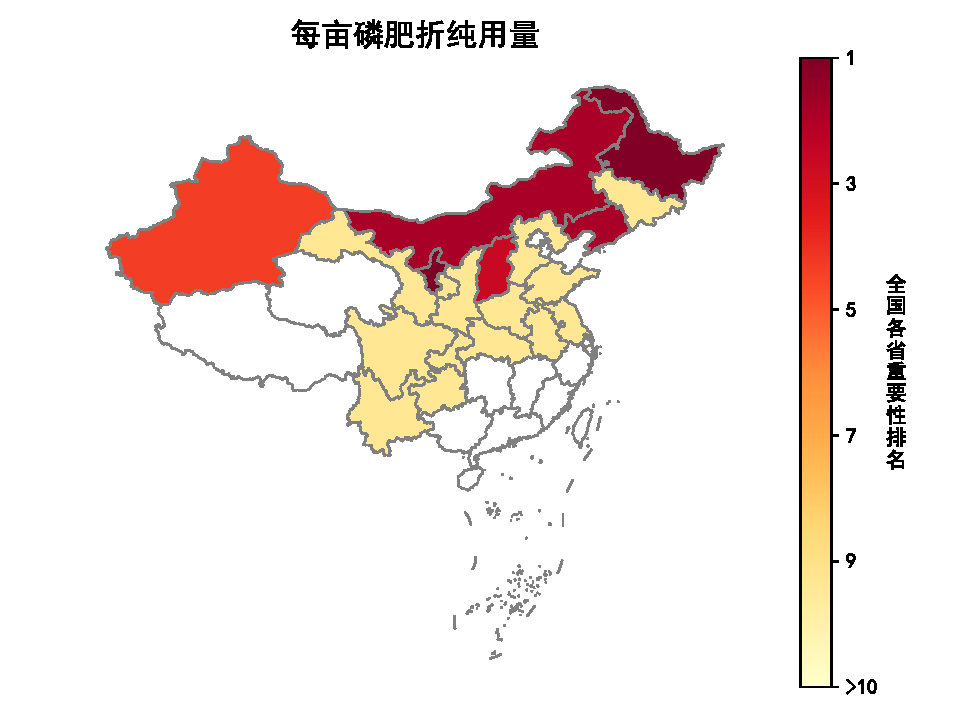
\includegraphics[width=\linewidth]{figs/NPK_P}
      \caption{磷肥}
      \label{fig:fertilizer_P}
    \end{minipage}
    \hfill
    \begin{minipage}[t]{0.49\linewidth}
      \centering
      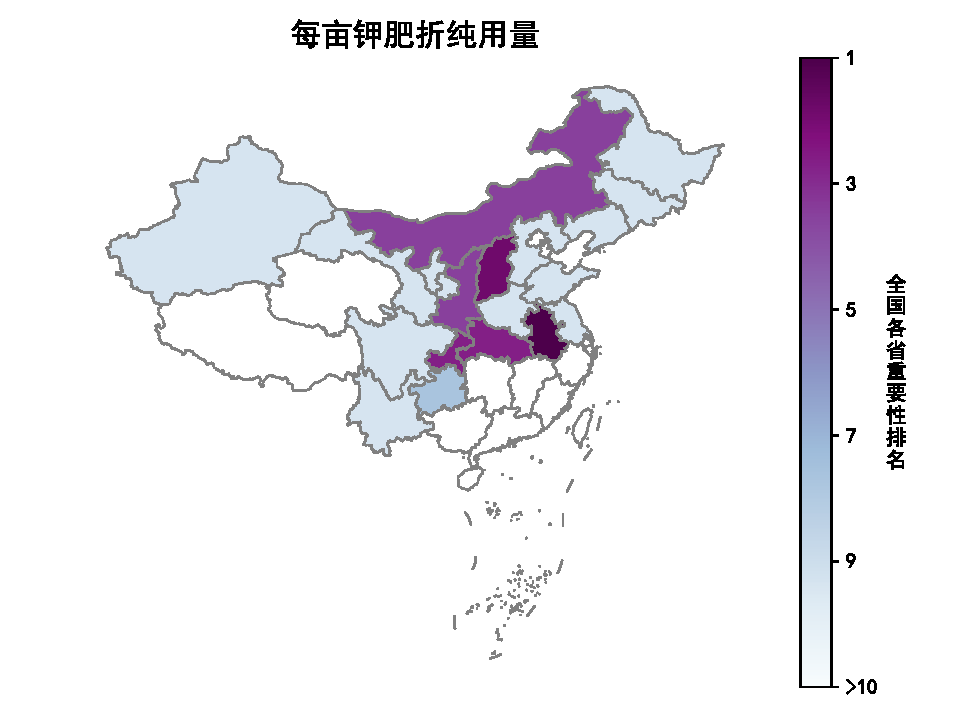
\includegraphics[width=\linewidth]{figs/NPK_K}
      \caption{钾肥}
      \label{fig:fertilizer_K}
    \end{minipage}
    \caption{每亩磷肥与钾肥折纯用量}
    \label{fig:fertilizer_PN}
  \end{figure}

从图中可以看出,磷肥与钾肥主要对个别集中的省份的影响较大。磷肥主要对东北省份及内蒙古、宁夏、山西影响较大,这可能与我国北方土地缺磷有关。钾肥主要对我国安徽、湖北、重庆等中南部地区及山西、陕西、内蒙古等北部省份影响较大。其中,磷肥与钾肥同时对内蒙古和山西玉米产量影响较大。

磷肥与钾肥对玉米产量的影响不同。玉米施用磷素化肥,穗粒数有明显增加。玉米施用钾素化肥增产的主要表现是提高百粒重,增加穗粒数\cite{施用氮磷钾肥对夏玉米产量和品质的影响}。磷肥的施入能够有效提升玉米产量,增加玉米种植经济效益,但过量施入磷肥会导致玉米产量及经济效益降低\cite{磷肥用量对玉米产量的影响}。因此在农业生产中应合理配施磷、钾肥, 促进养分比例的协调供给和保持养分平衡, 使玉米对磷、钾营养元素的吸收增多\cite{磷钾肥配合施用对玉米产量及养分吸收的影响}。在农业生产实践中,不同省份要根据其特定的土壤性质与气候条件,调整合理的磷钾肥使用量。而俄乌两国作为农作物肥料的主要供应国,占全球化肥出口贸易总额的近四分之一。在俄乌冲突导致全球化肥供应紧张的情况下,还应尽量保障图中磷钾肥对玉米生产较为重要的省份的供应充足,以此保障我国粮食生产与安全。


% \subsection{化肥投入情况}
% 化肥一直是农业生产中影响作物产量的重要因素,不同作物根据自身所需的营养物质与土壤的不同也会对不同种类化肥有着不同的需求。下面\ref{fig:fertilizer_PN}是磷肥与钾肥投入情况的重要度。
%   \begin{figure}[htb]
%     \centering
%     \begin{minipage}[t]{0.49\linewidth}
%       \centering
%       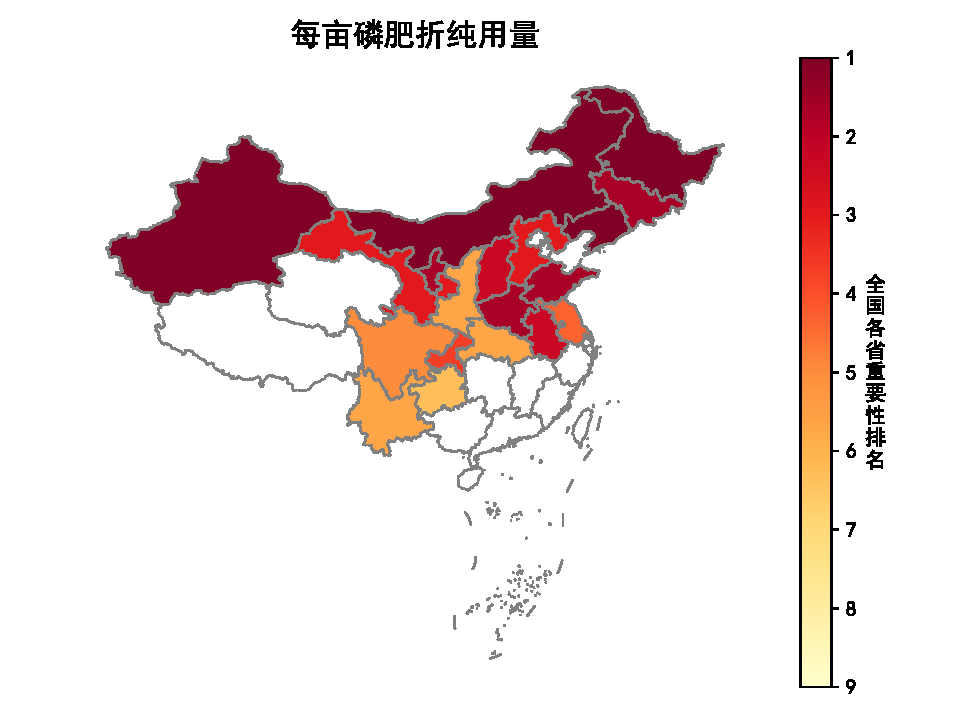
\includegraphics[width=\linewidth]{figs/fertilizer_P.pdf}
%       \caption{磷肥}
%       \label{fig:fertilizer_P}
%     \end{minipage}
%     \hfill
%     \begin{minipage}[t]{0.49\linewidth}
%       \centering
%       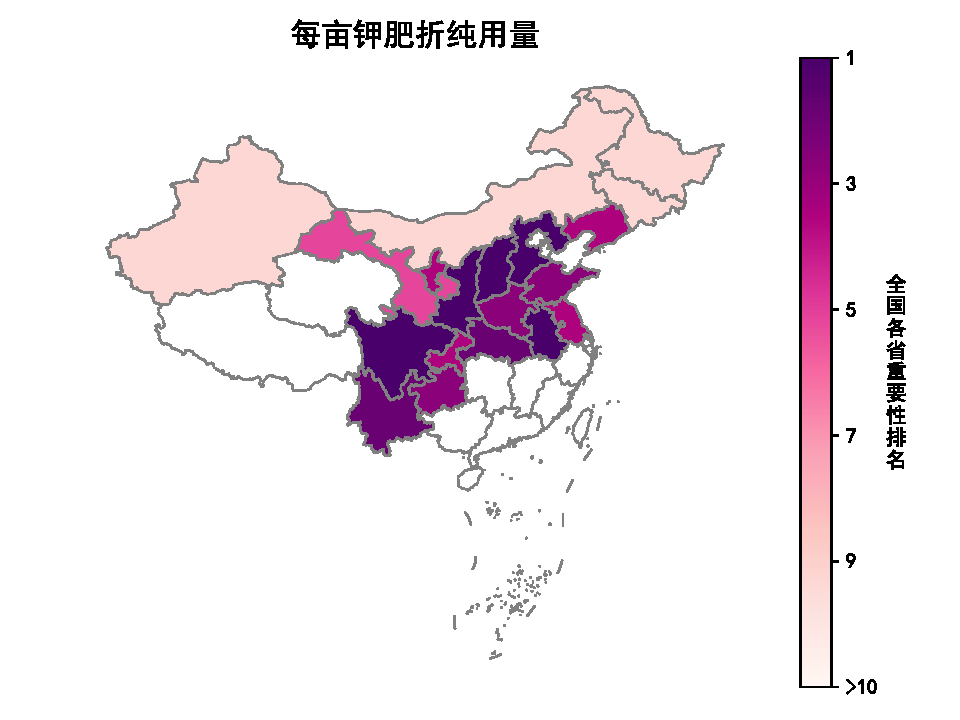
\includegraphics[width=\linewidth]{figs/fertilizer_K.pdf}
%       \caption{钾肥}
%       \label{fig:fertilizer_K}
%     \end{minipage}
%     \caption{每亩磷肥与钾肥折纯用量}
%     \label{fig:fertilizer_PN}
%   \end{figure}

% 从图中可以看出,钾肥与磷肥是影响玉米亩产的重要因素,其中磷肥在我国北方省份的重要程度集中在前3,钾肥在我国南方省份也有着相同的重要程度。而我国由于纬度跨度大地形复杂,南北方土壤的土壤肥力与营养元素含量也有着较大差异,图中结果恰好与我国北方土壤缺磷南方缺钾相应,也从侧面说明了本文实验结果的正确性。

% 图中结果显示在我国19个省份中磷肥钾肥在16个省份中占据了前三名的位置,说明磷肥钾肥在玉米生长过程中起着至关重要的作用,且南北方对两种化肥的需求不同,北方对磷肥需求大而南方对钾肥需求大,在农业生产实践中,南北方不同省份要根据其特定的土壤性质与气候条件,调整合理的磷钾肥使用量。而俄乌两国作为农作物肥料的主要供应国,占全球化肥出口贸易总额的近四分之一。在俄乌冲突导致全球化肥供应紧张的情况下,还应尽量保障北方磷肥与南方钾肥的供应充足,以此来保障我国粮食生产与安全。

% 本文实验数据中除了磷肥钾肥外,还包含了氮肥、复混肥、农家肥,其中\ref{fig:fertilizer_NF}展示了氮肥与农家肥投入情况的重要程度。

% \begin{figure}[htb]
%   \centering
%   \begin{minipage}[t]{0.49\linewidth}
%     \centering
%     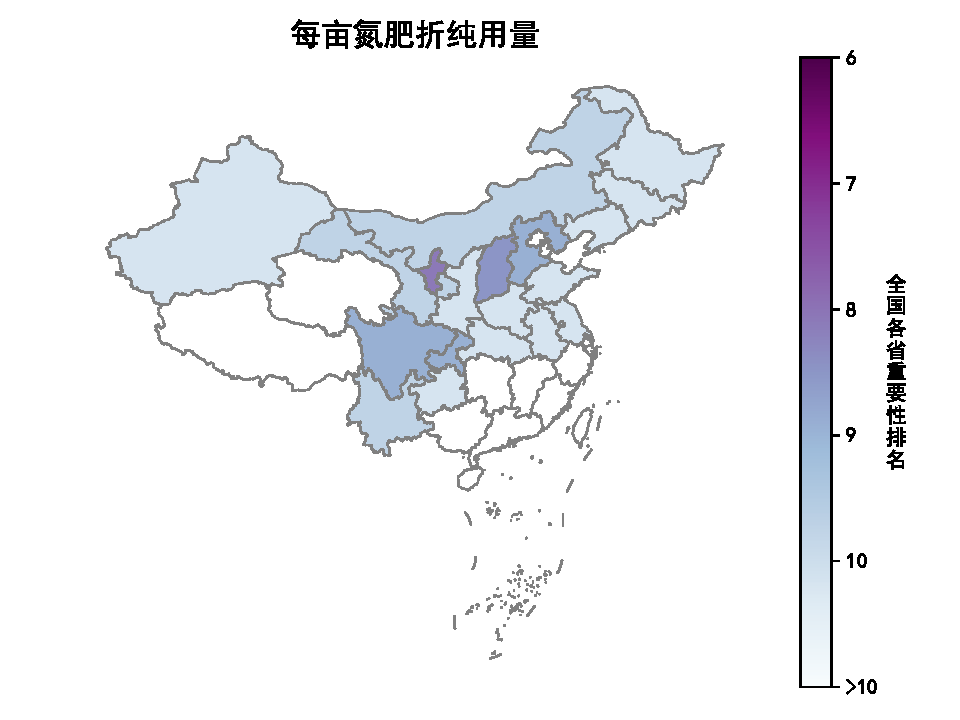
\includegraphics[width=\linewidth]{figs/fertilizer_N.pdf}
%     \caption{氮肥}
%     \label{fig:fertilizer_N}
%   \end{minipage}
%   \hfill
%   \begin{minipage}[t]{0.49\linewidth}
%     \centering
%     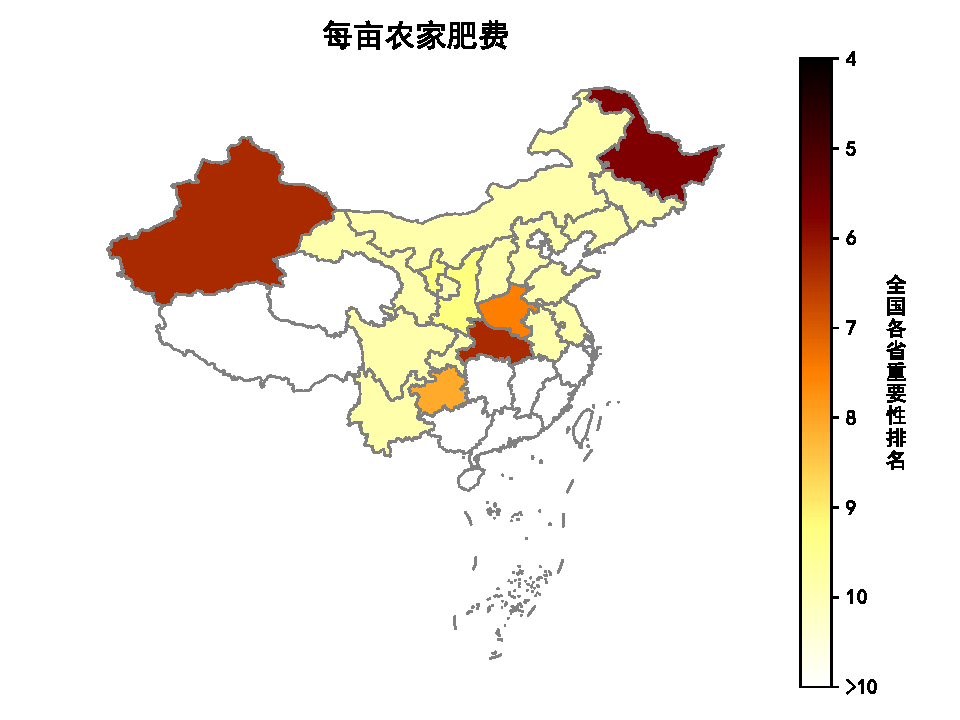
\includegraphics[width=\linewidth]{figs/fertilizer_farmyard.pdf}
%     \caption{农家肥}
%     \label{fig:fertilizer_farmyard}
%   \end{minipage}
%   \caption{每亩氮肥与农家肥折纯用量}
%   \label{fig:fertilizer_NF}

% \end{figure}

% 从图中可以看出,与磷肥钾肥大都集中在重要性前三不同,氮肥在全国重要性大都集中在第10名及以外,这可能是在大多数情况下,我国氮肥水平已经很高了,土壤中的氮素含量已经足够满足玉米生长的需要,过量的氮肥可能会对作物生长产生负面影响,因此氮肥对玉米产量的影响不大,在生产过程中注意适量施用氮肥。\cite{刘明鹏2022氮肥施用对四川紫色土矿质态氮淋失特征及春玉米产量的影响}然而复混肥作为一种混合肥料,其基本功能可以由其余氮磷钾肥相抵,在基本上所有省份中都没有进入重要性前10,对玉米产量并没有特别显著的影响。

% 而农家肥作为有机肥的一种,在实现有机农业、保护土地等方面有着重要的作用,其中以黑龙江黑土地为代表,其在自然条件下富含有机质且肥力高,而长期过度耕作和不合理的施肥方式都会导致土壤质量下降,因此保护黑土地非常重要。对于黑土地的管理和保护需要采取合理的耕作措施和施肥方案,充分利用农家肥等有机肥料可以保持土壤肥力和生产力的稳定,且农家肥在保护黑土地的同时,还能帮助农户节本增效。同理新疆因气候地理原因土地养分相对较少,施用农家肥可提高土地肥力改善土壤结构。因而在黑龙江、新疆等个别省份在农耕中要格外重视农家肥的影响。

% 因此建议农民在施用肥料时,做到因地制宜,根据当地土壤质量和作物需求的不同,适量施用农家肥,达到肥料的最佳配比,提高农业生产的效益和可持续性。

% \subsection{自然灾害}

% \begin{figure}[htb]
%   \centering
%   \begin{minipage}[t]{0.49\linewidth}
%     \centering
%     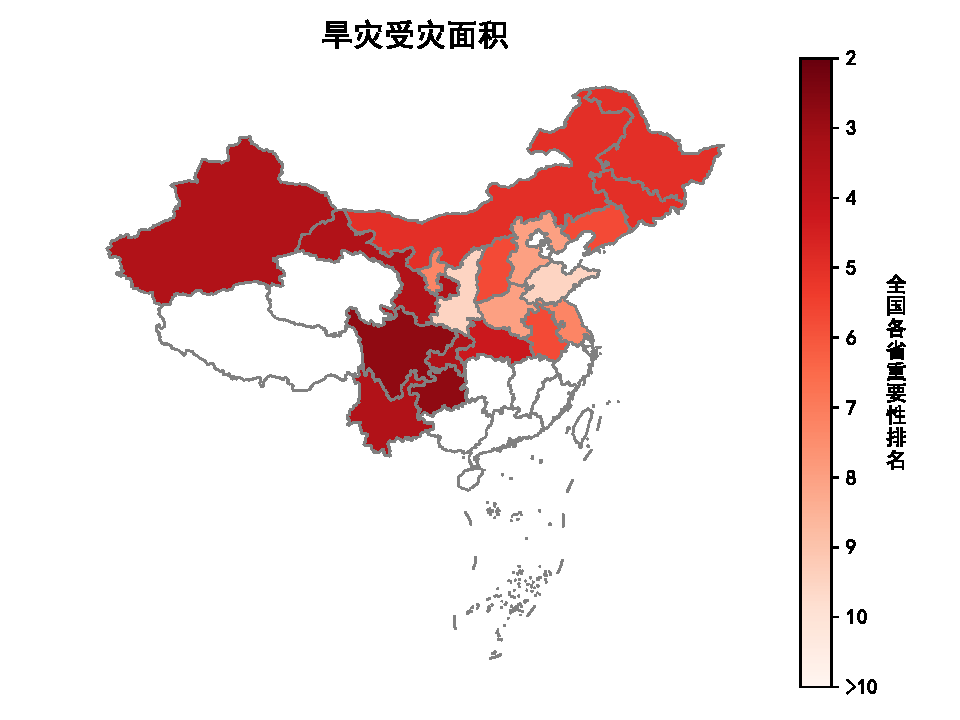
\includegraphics[width=\linewidth]{figs/hazard_drought.pdf}
%     \caption{旱灾}
%     \label{fig:hazard_drought}
%   \end{minipage}
%   \hfill
%   \begin{minipage}[t]{0.49\linewidth}
%     \centering
%     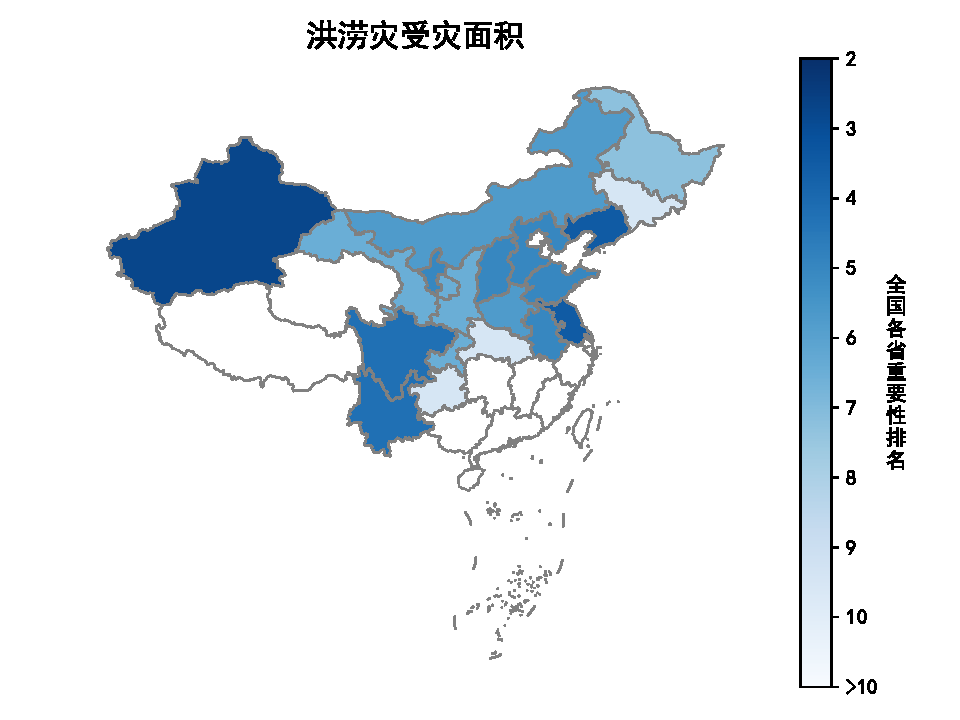
\includegraphics[width=\linewidth]{figs/hazard_flood.pdf}
%     \caption{洪涝灾}
%     \label{fig:hazard_flood}
%   \end{minipage}
%   \caption{旱灾与洪涝受灾面积}
%   \label{fig:hazard}
% \end{figure}

% 自然灾害作为影响作物生长的直接因素,直接影响着受灾地区作物的生长与丰收。而旱灾与洪涝灾害作为最常见的灾害,分析其主要影响区域对于作物种植有着重要意义。\ref{fig:hazard}展示了全国各省旱灾洪灾影响因子的重要性排名。

% 图中结果展示了我国旱灾与洪涝灾害对玉米产量有着非常大的影响,在近一半省份中均排在了重要性前5。其中中国西部的西南农业区受旱灾影响最严重,例如四川、贵州、新疆等地的常年遭遇旱灾,对当地农作物的生长有着较大的影响。此外,我国新疆、西南地区及辽宁江苏等沿海省份受到洪涝灾害影响也较严重,对玉米的生长及产量有着较大的影响。

% 其中四川、云南位于中国西南地区,虽属于亚热带季风气候区域,但由于受到地形和气候的影响,这些地区的降雨量和水资源分布非常不均衡,同时也对排灌设施的建设和维护带来了较大困难,造成了干旱和水灾等自然灾害的频繁发生。对于新疆而言,其地理位置位于亚欧大陆腹地,是典型的内陆干旱地区,旱灾频繁发生,但因其三山夹两盆的特殊地形和独特的自然环境格局,同时较容易受到洪涝灾害的严重影响。\cite{哈斯也提·热合曼2020新疆}

% 对于新疆、四川、云南等省份而言,两种灾害对玉米产量的影响因素基本全排在重要性前4位,说明这两种自然灾害作为影响玉米生产的重要因素,已经对其产量产生了较为严重的负面影响。因此对于容易受到旱灾影响的省份,应加强土地的水分管理,提高灌溉效率,减少土地退化和干旱损失。对于容易受到洪涝灾害影响的省份,建议加强防洪和排灌设施的建设,提高其应急响应能力。因在不同省份旱灾和洪涝灾害对玉米产量的影响各不相同,各省份应根据其本身的气候特点和土地条件,采取相应的防范措施。

\subsection{成本投入情况}
\begin{figure}[htb]
  \centering
  \begin{minipage}[t]{0.49\linewidth}
    \centering
    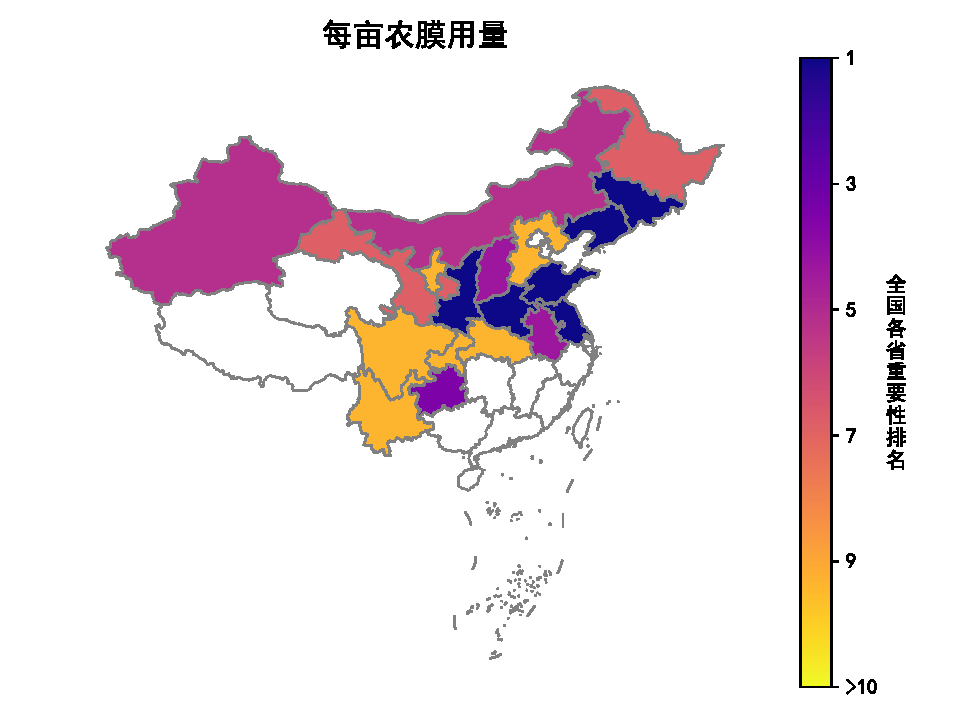
\includegraphics[width=\linewidth]{figs/InputCost_Film}
    \caption{农膜投入}
    \label{fig:InputCost_Film}
  \end{minipage}
  \hfill
  \begin{minipage}[t]{0.49\linewidth}
    \centering
    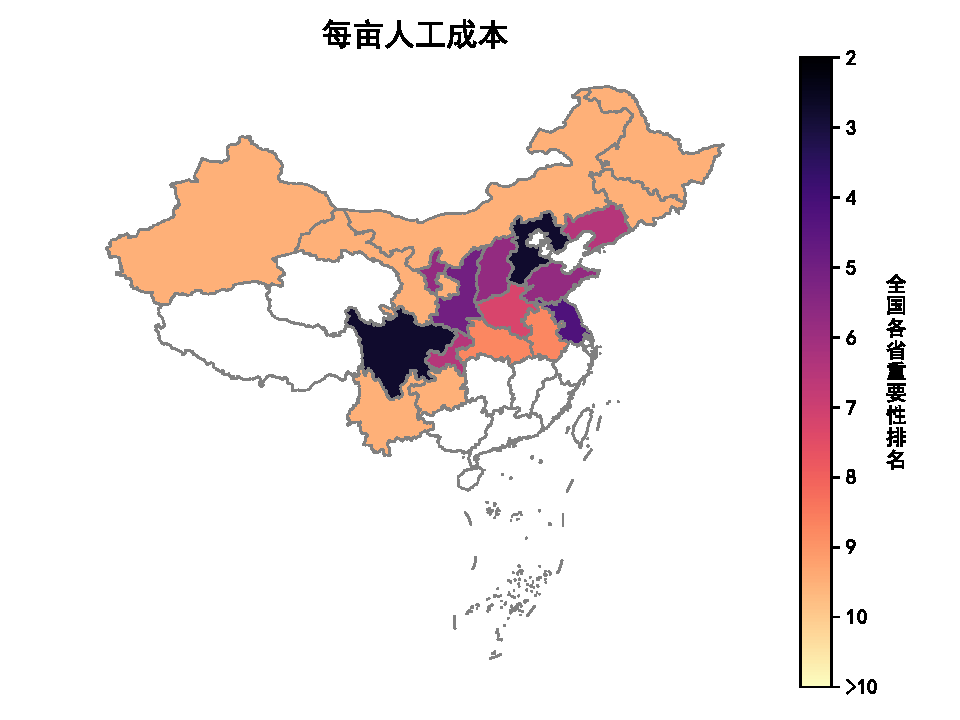
\includegraphics[width=\linewidth]{figs/InputCost_Labor}
    \caption{人工成本}
    \label{fig:InputCost_Labor}
  \end{minipage}
  \caption{成本投入情况}
  \label{fig:input_FL}
\end{figure}

在成本投入情况中,每亩农膜用量与每亩人工成本对玉米产量有着较为重要的影响。因此\ref{fig:input_FL}中展示了这两个变量的重要程度。

20世纪80年代初我国开始应用农作物地膜覆盖技术,地膜覆盖技术可以起到增温保湿作用, 使农作物增产的同时也提高了农产品品质, 为社会带来巨大的经济效益。然而过多的农膜残留在土壤中也增加了清膜成本, 同时又会破坏土壤结构\cite{可降解农膜在玉米上的应用研究}。因此对于每亩农膜用量而言,收成并不一定与用量成正比。如果每亩农膜用量过多,会导致土壤过于密封,通气性差,不利于农作物的根系呼吸,容易发生病虫害,且会阻碍水分和养分的渗透,影响农作物的吸收和利用,同时不可降解农膜还会破坏土壤结构造成环境污染。而如果每亩农膜用量过少,会无法达到良好的保温、保湿、杀菌和抗旱效果,容易导致农作物受到干旱和低温等自然灾害的影响,产量和质量也会受到影响。由\ref{fig:InputCost_Film}可得,我国陕西、河南、内蒙古、新疆等中西部省份可能由于土壤、气候等因素导致水分养分蒸发流失较快,因而适量增加农膜使用可以保持水分、养分和温度。而吉林、辽宁、山东、江苏等东北及沿海地区由于气候湿度等原因,使用农膜可以一定程度上保持温度与湿度,进而提高产量。因而在沿海地区与中西部地区在玉米种植过程中要注意合理使用农膜。

每亩人工成本代表的是农业生产中的劳动力市场情况与农业机械化程度。一般来说每亩人工成本的重要性越高,意味着该地区玉米生产对于人工劳动力的依赖程度越高,农业机械化程度较低,同时说明农业劳动力市场较为匮乏。由\ref{fig:InputCost_Labor}可得,每亩人工成本对四川、河北玉米产量有着很大的影响,对陕西、山东、江苏等中部及沿海省份也有着较大的影响,这与发达省份人工劳动力成本高及农业机械化程度均有关。因而对于劳动力市场人工成本较高的省份应注意提高农业机械化的建设与发展,减少对人工劳动力的依赖;对于地形复杂耕作成本较高的地区,可以通过提高农业机械化水平与加大人工劳动力投入来提高玉米产量。

% \subsection{物化投入情况}
% \begin{figure}[htb]
%   \centering
%   \begin{minipage}[t]{0.49\linewidth}
%     \centering
%     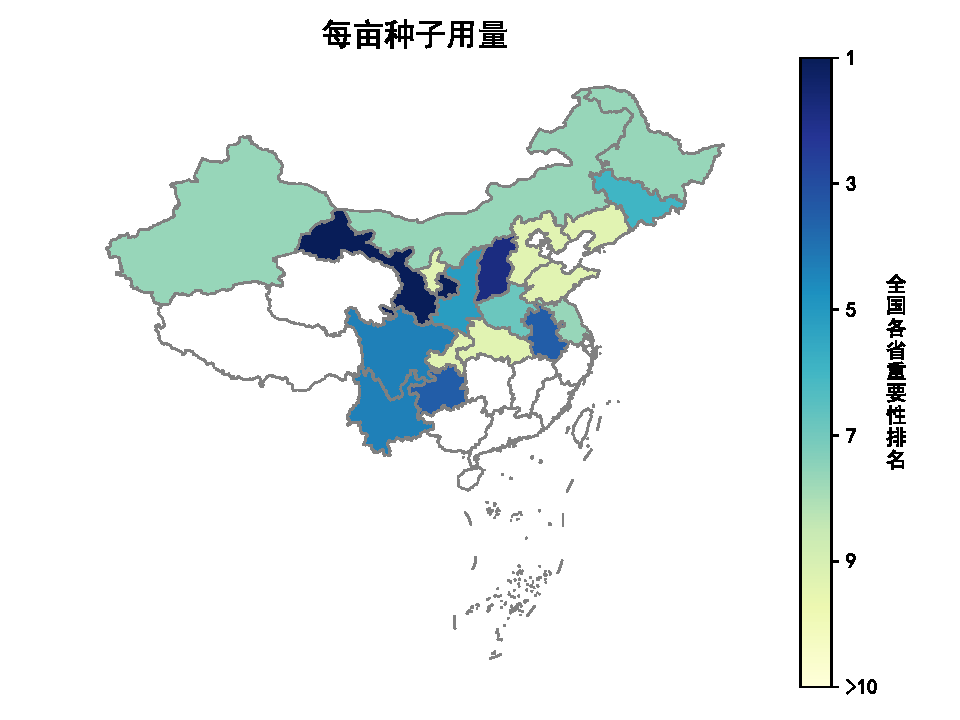
\includegraphics[width=\linewidth]{figs/input_Seeds.pdf}
%     \caption{种子}
%     \label{fig:input_Seeds}
%   \end{minipage}
%   \hfill
%   \begin{minipage}[t]{0.49\linewidth}
%     \centering
%     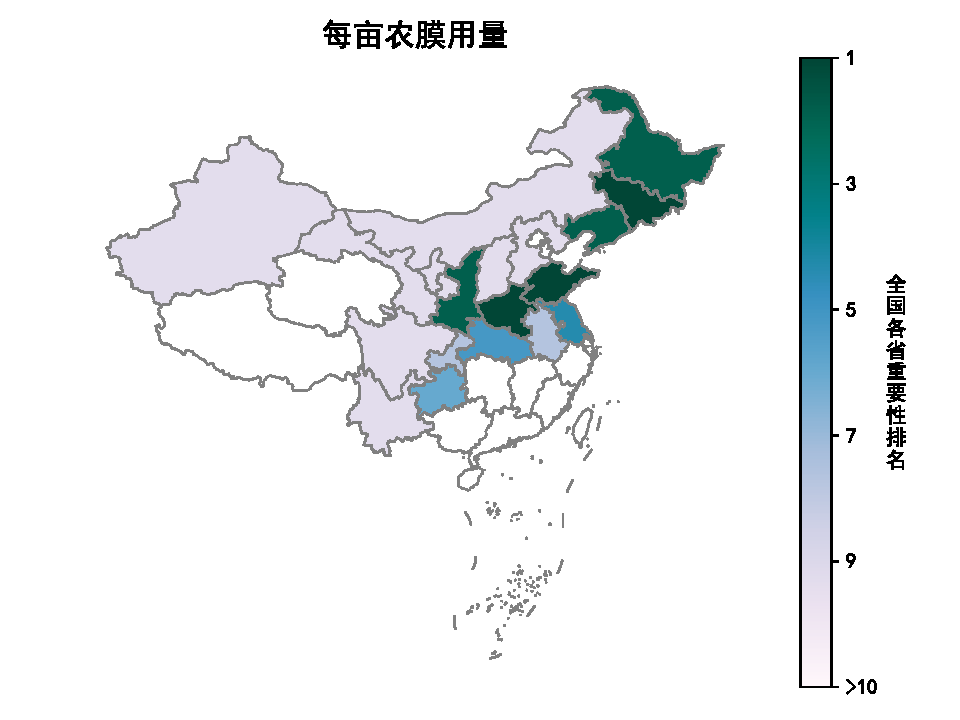
\includegraphics[width=\linewidth]{figs/input_AgriFilm.pdf}
%     \caption{农膜}
%     \label{fig:input_AgriFilm}
%   \end{minipage}
%   \caption{物化投入情况}
%   \label{fig:input_AS}
% \end{figure}

% 在物化投入情况中,仅有每亩种子用量和每亩农膜用量这两个变量在全国各省中具有较为重要的排名。因此\ref{fig:input_AS}中展示了这两个变量的重要程度。而解释变量玉米播种面积在各省重要性排名中均为进入前10,恰好印证了玉米的亩产与播种面积无关。


% 对于每亩种子用量来说,其收成与用量并不是成正比。如果每亩种子用量过多,会导致种植密度过高,单株营养面积小,影响作物之间的空间竞争,从而降低产量和质量,且造成种子浪费增加农民成本。如果种子用量过少,每亩土地难以保证应有的苗数,降低产量的同时还会降低土地利用效率。因而由\ref{fig:input_Seeds}可得甘肃、山西、贵州等中西部地区在玉米种植过程中要进行合理密植,科学选择每亩种子用量。\cite{董云2015填充物与用种量对机械化条播油菜群体质量及产量的影响}


% 对于每亩农膜用量而言,收成也并不一定与用量成正比。如果每亩农膜用量过多,会导致土壤过于密封,通气性差,不利于农作物的根系呼吸,容易发生病虫害,且会阻碍水分和养分的渗透,影响农作物的吸收和利用,同时还会造成环境污染。而如果每亩农膜用量过少,会无法达到良好的保温、保湿、杀菌和抗旱效果,容易导致农作物受到干旱和低温等自然灾害的影响,产量和质量也会受到影响。由\ref{fig:input_AgriFilm}可得,山东、河南、陕西等地区可能由于土壤、气候等因素导致水分养分蒸发流失较快,因而适量增加农膜使用可以保持水分、养分和温度。而东北三省地区较为寒冷,使用农膜可以一定程度上提高土壤温度,进而提高产量。因而在东北三省地区与中原地区在玉米种植过程中要注意合理使用农膜。

\subsection{排灌建设情况}

\begin{figure}[htb]
    \centering
    \begin{minipage}[t]{0.49\linewidth}
      \centering
      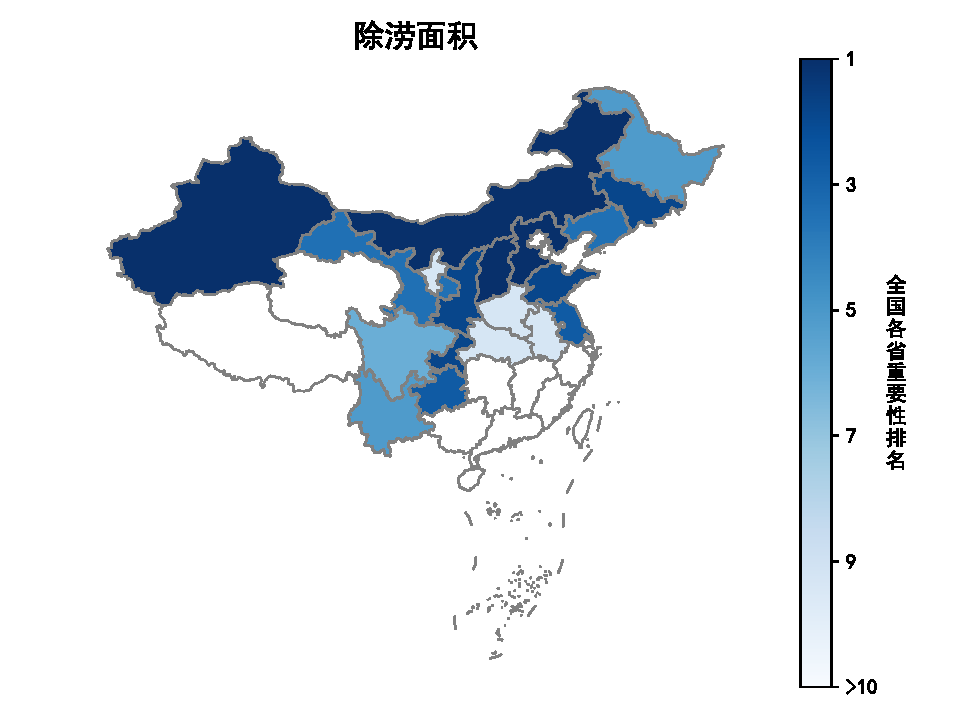
\includegraphics[width=\linewidth]{figs/DrainIrrigate_WaterLogging}
      \caption{除涝面积}
      \label{fig:DrainIrrigate_WaterLogging}
    \end{minipage}
    \hfill
    \begin{minipage}[t]{0.49\linewidth}
      \centering
      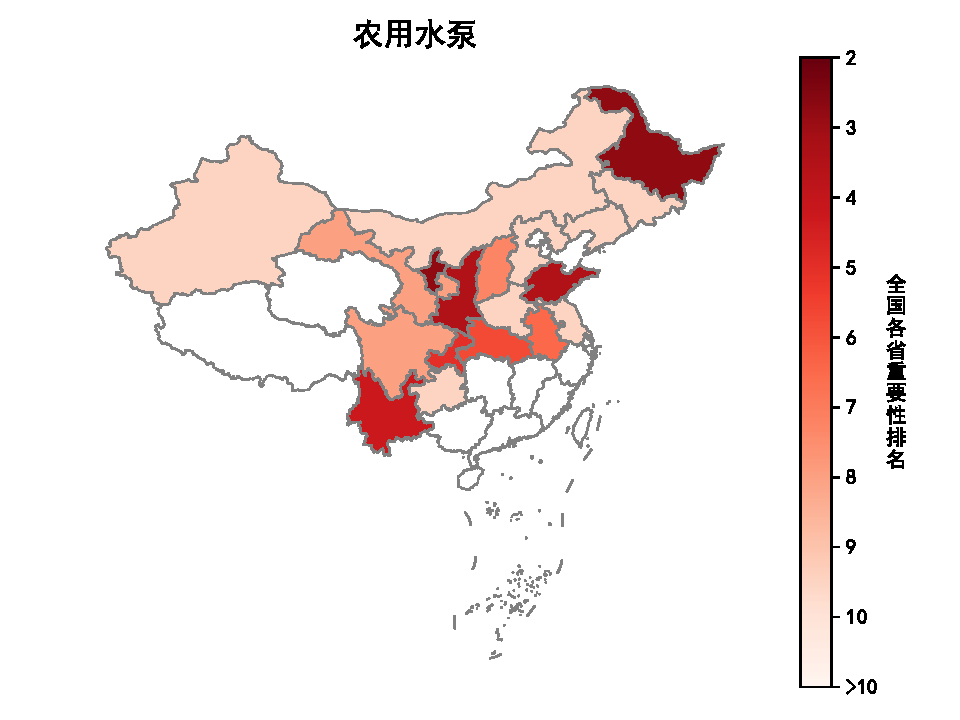
\includegraphics[width=\linewidth]{figs/DrainIrrigate_WaterPump}
      \caption{农用水泵}
      \label{fig:DrainIrrigate_WaterPump}
    \end{minipage}
    \caption{排灌建设情况}
    \label{fig:DrainIrrigate}
  \end{figure}

  在排灌建设情况中,除涝面积代表着排水情况,农用水泵数代表着灌溉情况,因此\ref{fig:DrainIrrigate}中展示了这两个变量的重要程度。

  \ref{fig:DrainIrrigate_WaterLogging}显示除涝面积对于我国新疆、内蒙古、山西、河北等中西部省份及部分沿海省份的玉米生产影响较大,除涝面积的大小对于保护和维持玉米生产的稳定性具有重要作用,增加除涝面积可以减少因洪涝灾害而导致的玉米受灾面积和产量损失。对于受到除涝面积影响大的省份,说明雨涝洪涝在这些省份对于玉米的生长产生了较大的影响,因而在生产过程中格外注意在雨涝洪涝后及时开展除涝补救措施,以减少因雨涝导致的玉米减产\cite{东北三省地区生长季旱涝对春玉米产量的影响}。
  
  而\ref{fig:DrainIrrigate_WaterPump}显示农用水泵对于我国黑龙江、宁夏、陕西、云南、山东等个别省份的玉米生产有较大的影响。农用水泵反映着农业生产中的灌溉水平与规模,对于农用水泵在玉米生产中有着较高重要度的省份,说明该地区因气候环境土壤等原因导致玉米生长对于灌溉设施有着较大的依赖,在玉米生产中这些地区要格外重视灌溉设施的建设与完善,加强灌溉设施的投入力度,优化农田水利设施建设,提高灌溉效率和节水利用,并在旱季加大对玉米的灌溉力度,避免因灌溉不足而导致的减产发生。

  根据排灌建设情况对不同省份玉米产量的影响,可以得出水分对玉米生长有着重要的影响。对于受到影响较大的省份,政府应该加大对这些地区的排灌设施建设和维护力度,提高排灌设施的效率与覆盖面积。对于受到排灌费影响较小的地区,也应加强设施的完善与维护,同时应鼓励农民使用节水灌溉技术,尽可能降低排灌成本与节约用水量。

  \subsection{机械化建设情况}
  \begin{figure}[htb]
      \centering
      \begin{minipage}[t]{0.49\linewidth}
        \centering
        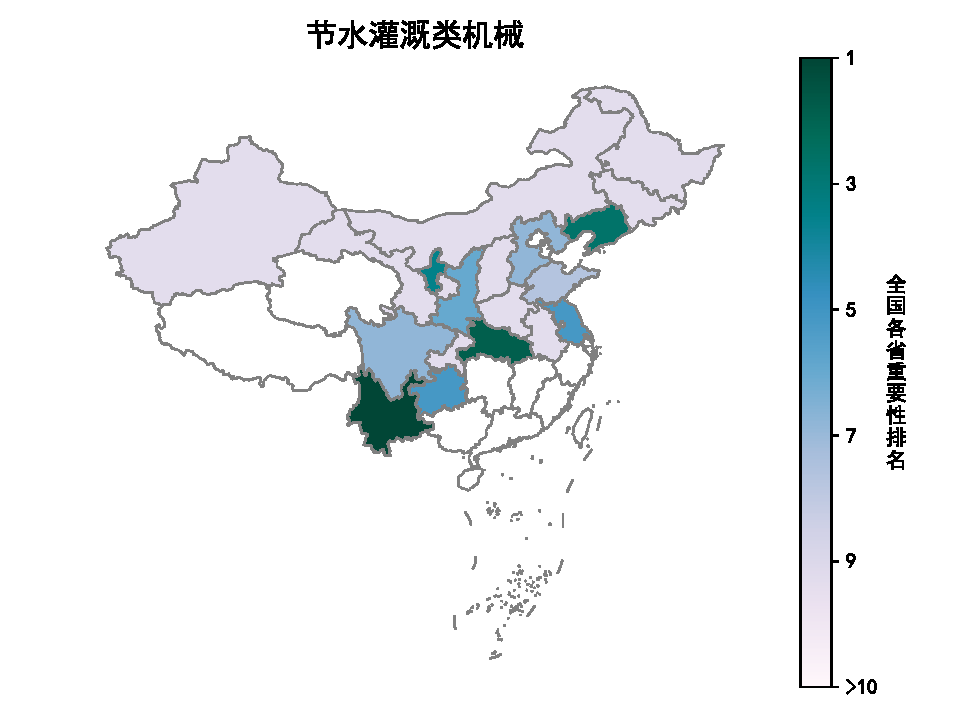
\includegraphics[width=\linewidth]{figs/Mechanization_IrrigationMachinery}
        \caption{灌溉机械}
        \label{fig:Mechanization_IrrigationMachinery}
      \end{minipage}
      \hfill
      \begin{minipage}[t]{0.49\linewidth}
        \centering
        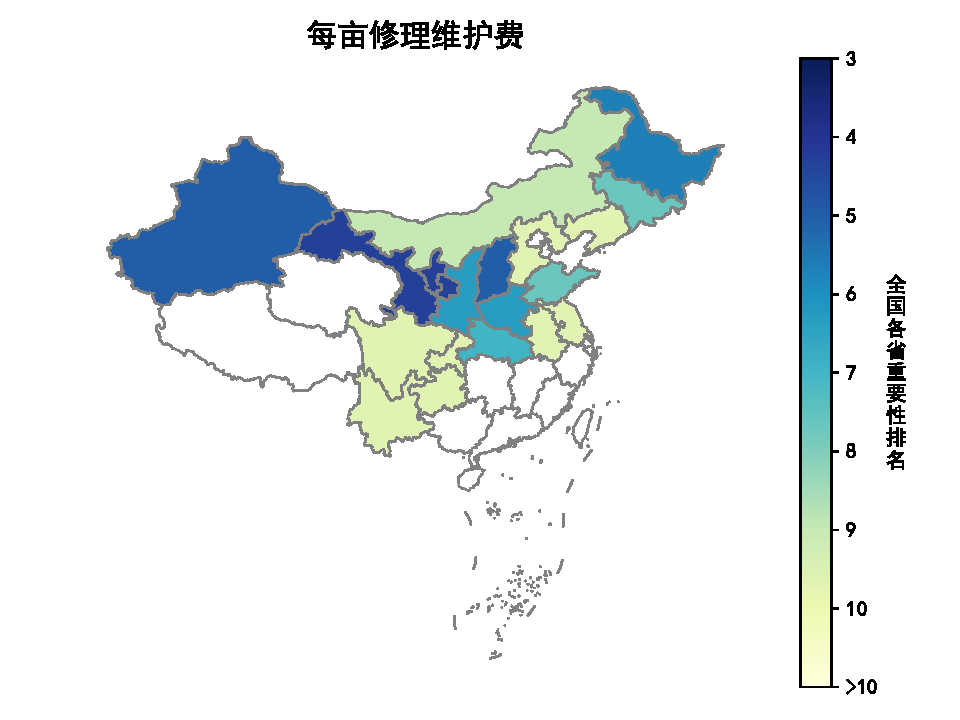
\includegraphics[width=\linewidth]{figs/Mechanization_Repair}
        \caption{修理维护}
        \label{fig:Mechanization_Repair}
      \end{minipage}
      \caption{机械化建设情况}
      \label{fig:Mechanization}
    \end{figure}

在机械化建设情况中,一个地区农用机械拥有量可以反映其农业机械化发展程度。节水灌溉类机械作为农业机械中关键的一部分,是指在农业生产中用于提高灌溉效率、减少用水量的设备和工具。一个地区节水灌溉类机械持有量越多代表着该地区农业灌溉机械化与自动化越发达。每亩修理维护费主要反映了农业机械设备的使用情况和维护保养水平。如果农业机械设备使用频率高、年限长、维护保养不及时,就会导致每亩修理维护费增加。因此节水灌溉机械持有量可以反映某地区机械化的体量与发展程度,而每亩修理维护费可以反映某地区灌溉机械的设备可靠性、生产稳定性及灌溉效率与成本。研究表明我国玉米灌溉属国际较低水平,水分对玉米的生长起着至关重要的作用,是影响玉米最终产量的重要因素,因此, 在进行玉米灌溉时应尽量选择灌溉效果较好的方式进行作业, 节水灌溉机械化播种作业技术就是一种提升玉米出苗率、玉米产量的有效方法\cite{浅谈玉米节水灌溉机械化播种作业技术}。

对于节水灌溉类机械,如\ref{fig:Mechanization_IrrigationMachinery}中结果所示,其对我国云南、湖北、宁夏、辽宁等省份的玉米产量有着较大影响,针对地形复杂与发展相对落后的地区,加强节水灌溉设施建设将有助于提高农业机械化程度,进而显著提高生产效率。针对气候干旱的地区,由于水分对玉米的生长有着重要的作用,因此加大节水灌溉机械的建设力度能够在旱季中保持玉米生长的水分需求,避免了因干旱导致的减产。

对于每亩修理维护费,由\ref{fig:Mechanization_Repair}可以看出,每亩修理维护费对我国甘肃、宁夏、新疆、山西、黑龙江等省份的玉米生产影响较大。每亩修理维护费相较于节水灌溉类机械,可以反映生产设备的质量、维护管理的水平及生产环境的条件。针对这些对玉米生产影响较大的省份,在购买农业机械设备时优先选择质量可靠、耐用性好的设备,并加强农业机械设备的维护管理工作,定期进行检查和保养,同时改善农田环境条件,以减少机械设备在作业过程中的损耗和故障风险。通过减少农业生产中的农业机械的损耗,有助于降低修理维护费用,提高玉米农业生产效益。




% 每亩修理维护费主要反映了农业机械设备的使用情况和维护保养水平。如果农业机械设备使用频率高、年限长、维护保养不及时,就会导致每亩修理维护费增加。

% 由\ref{fig:rural_investment}可以看出,对于沿海地区和川渝地区等发达地区,农业机械设备的使用情况和维护保养水平相对较高,因此每亩修理维护费对玉米产量的影响较低。而对于云南、内蒙古、河南内陆且对农业机械依赖度较大的省份,由于地理位置和自然环境等因素的影响,农业机械设备的使用情况和维护保养水平可能较低,所以每亩修理维护费对玉米产量的影响较大。

% 针对这一结果,我们需要在制定政策时重视农业机械设备的使用和维护保养,促进农业机械化水平的提高,降低每亩修理维护费用,从而提高玉米产量和农民收益。同时,也需要注意发达地区与欠发达地区的差异,有针对性地制定政策,促进农业机械化的均衡发展。

% \subsection{农资投入情况}
% \begin{figure}[htb]
%   \centering
%   \begin{minipage}[t]{0.49\linewidth}
%     \centering
%     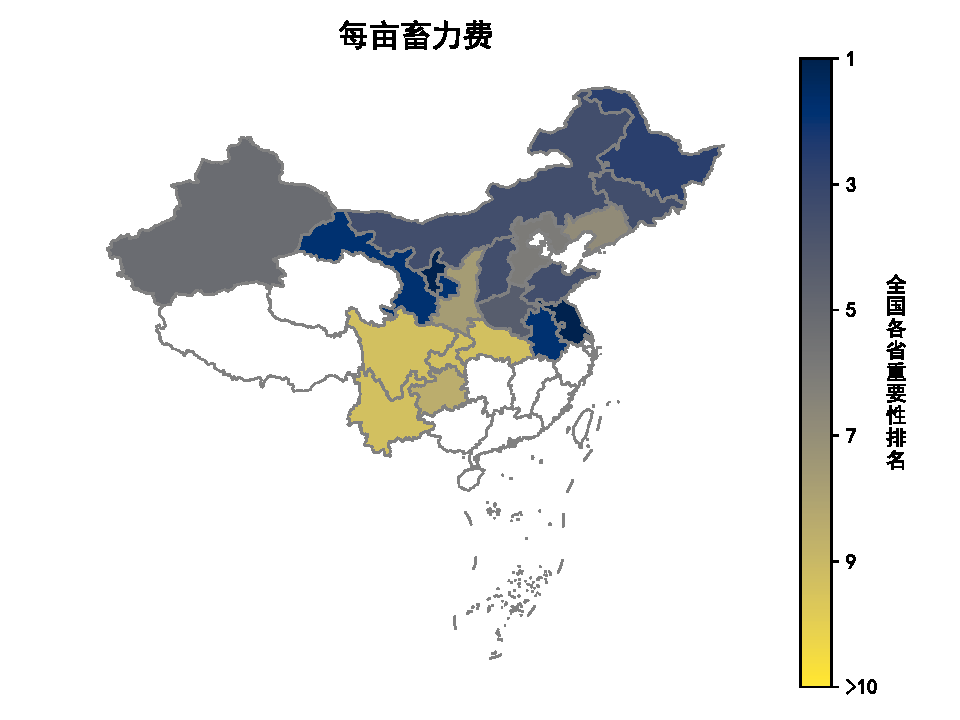
\includegraphics[width=\linewidth]{figs/cost_AniPower.pdf}
%     \caption{畜力费}
%     \label{fig:cost_AniPower}
%   \end{minipage}
%   \hfill
%   \begin{minipage}[t]{0.49\linewidth}
%     \centering
%     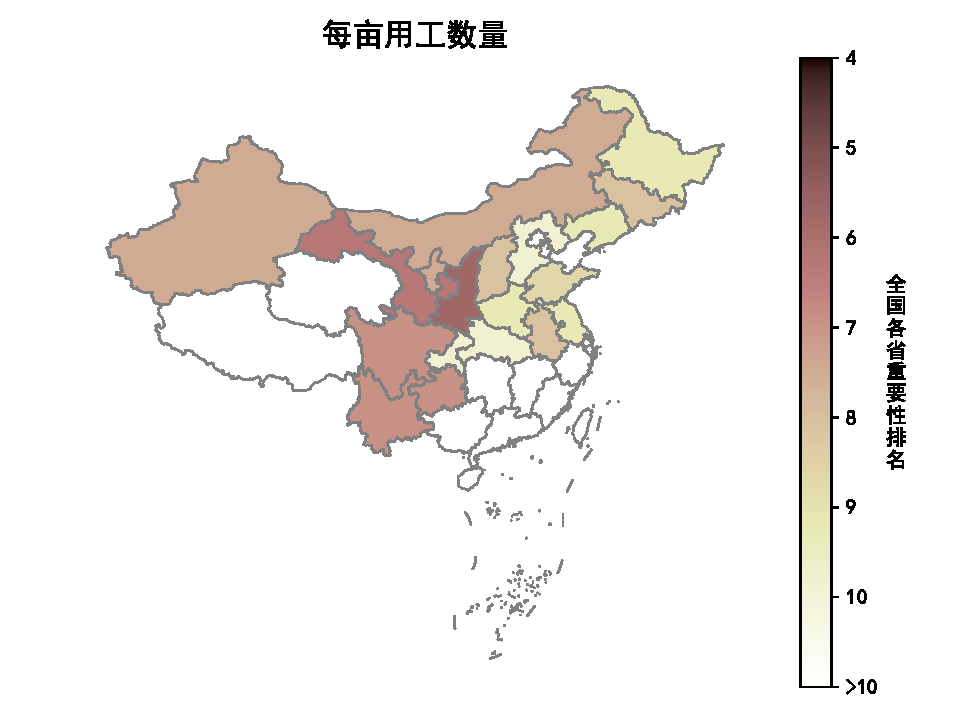
\includegraphics[width=\linewidth]{figs/cost_employ.pdf}
%     \caption{用工数}
%     \label{fig:cost_employ}
%   \end{minipage}\\[1em]
%   \begin{minipage}[t]{0.49\linewidth}
%     \centering
%     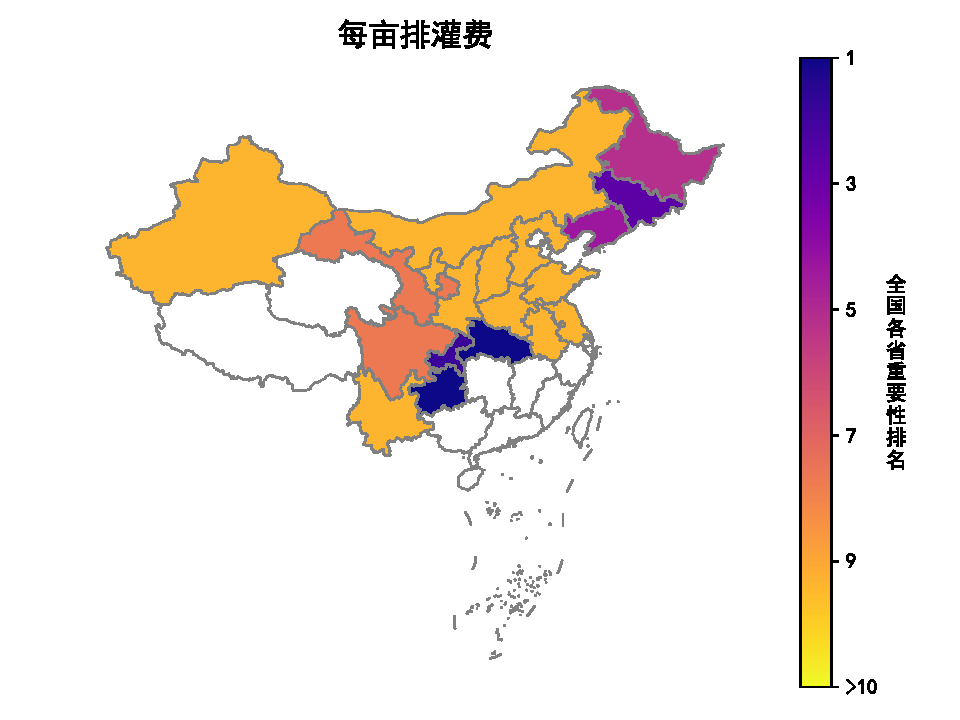
\includegraphics[width=\linewidth]{figs/cost_irrig.pdf}
%     \caption{排灌费}
%     \label{fig:cost_irrig}
%   \end{minipage}
%   \hfill
%   \begin{minipage}[t]{0.49\linewidth}
%     \centering
%     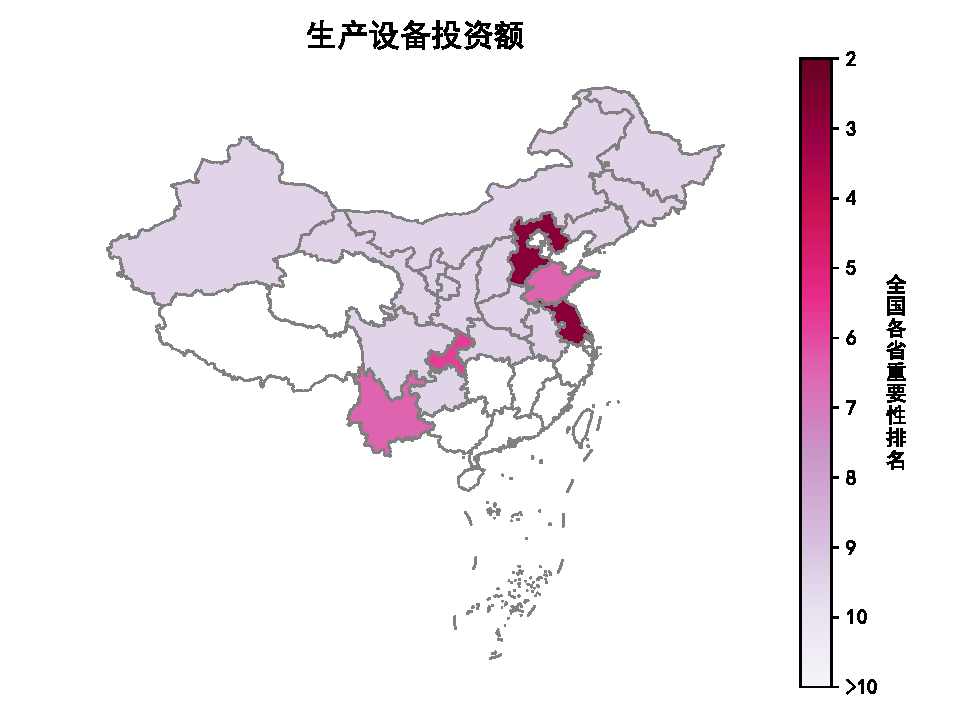
\includegraphics[width=\linewidth]{figs/rural_investment.pdf}
%     \caption{投资额}
%     \label{fig:rural_investment}
%   \end{minipage}
%   \caption{农资投入情况}
%   \label{fig:cost}
% \end{figure}

% 对于生产中投入的农资情况,在大多数省份中并不作为主要影响因素,只在少数省份中占主要影响因素。\ref{fig:cost}展示了相对最重要的4个因素作为分析对象,其余解释变量对玉米产量的影响重要性并不明显。

% \subsubsection{每亩畜力费}
% 每亩畜力费是一个综合的指标,涵盖了使用牲畜、畜力机械以及与其相关的各种费用。这个指标可以帮助了解在农业生产中使用畜力机械和牲畜所需的实际成本,进而对农业生产的投入和效益进行合理的分析。

% 一个地区的畜力费越高代表着其农业生产成本越高,而每亩畜力费在作物产量影响因素中越重要代表着在农业生产活动受到畜力费变化的影响较大,说明农业生产受到生产成本变化较严重。

% 由\ref{fig:cost_AniPower}可以看出,每亩畜力费在全国北方的重要性要远高于南方,考虑到北方地区的气候和土地条件相对于南方地区而言更加干旱,土地更加贫瘠,生产成本较高,因而在统筹农业生产规划的过程中需要注意我国南北方间生产成本的差异。

% \subsubsection{每亩用工数量}

% 每亩用工数量代表的是农业生产中的人工生产成本与人工生产效率,代表着农业生产的劳动力市场情况与农业机械化程度。由\ref{fig:cost_employ}可以明显看出,东部沿海地区普遍重要度较低,西部内陆地区重要度较高,说明由于我国东西部土地类型、气候条件、农业生产方式、农业机械化水平的不同,进而使得东部农业生产人工生产需求较低,西部相对较高。在西部地区农业劳动力的充足程度较低,而东部地区农业劳动力充足程度较高,农村劳动力市场在不同地区间产生了较大差异。

% 因此针对每亩用工数量对玉米产量的影响,应充分考虑地区间劳动力市场的差异,尽量减少我国东西部农村生产水平与生产成本的差异,可以通过推广农业机械化、提高农村生产条件、降低用工成本等减少每亩用工数量对玉米产量的限制,提高生产效率,从而提高玉米产量。

% \subsubsection{每亩排灌费}
% 每亩排灌费是指在农业生产中为了灌溉或排水而支出的费用。灌溉条件的好坏对产量有着重要的影响,同时排灌条件的建设与维护也需要耗费相应的资金与资源。

% 由\ref{fig:cost_irrig}可以看出,由于贵州、湖北、重庆等地区由于地形复杂气候湿润,对灌溉需求较大,灌排设施的建设难度较大,排灌系统建设费用相对较高,使得每亩排灌费对农业生产的影响程度较高。同时由\ref{fig:hazard_drought}中洪涝灾对玉米产量重要程度可得,贵州、湖北、重庆三省的玉米产量受到旱灾影响较为严重,这也间接说明了在这些省份排灌设备对而对于东北三省,气候较为寒冷,灌溉水源主要依靠人工补充,灌排系统对于低温和冻害等的应对需求较高,因此需要较高的排灌费用来保证农田的灌溉和排水,所以每亩排灌费对玉米产量的影响也更大。其他地区因地形或自然环境因素,对排灌需求不大或排灌设施已然完善,每亩排灌费对其玉米产量的影响便相对不特别重要。\cite{zhu2022investigating}

% 根据每亩排灌费对不同省份玉米产量的影响,可以得出排灌设施对农作物产量的重要性。对于受到排灌影响较大的省份,政府应该加大对这些地区的排灌设施建设和维护力度,提高排灌设施的效率与覆盖面积。对于受到排灌费影响较小的地区,也应加强设施的完善与维护,同时应鼓励农民使用节水灌溉技术,尽可能降低排灌成本与节约用水量。

% \subsubsection{生产设备投资额}

% 生产设备投资额是指在农业生产中用于购买和维护各种生产设备的资金支出,如农机具、灌溉设备等。在玉米产量影响因素中,生产设备投资额反映了农村在农业生产中采用现代化生产手段的程度和投入程度。\ref{fig:rural_investment}展示了生产设备投资额对各省玉米产量的影响重要程度。

% 农村生产设备投资额对玉米产量的影响主要与机械化水平、种植方式、技术水平等因素相关。河北、江苏等地区经济发达,农业机械化水平高,技术水平较高,因此农村生产设备投资额对其影响最大。而在其余一些影响不大的地区,可能由于农业现代化程度相对较低,生产设备投资对当地玉米产量提高的潜力仍未被充分发挥。

% 因此,政府还需加大对农村生产设备的投入,促进现代农业的发展,加大农业现代化建设力度,提高农业机械化水平和农业生产自动化程度。同时根据不同地区的实际情况,合理规划农村生产设备的投资方向和数量,确保投入有序和合理。最后还要加强对农业生产设备的研发和技术创新,推广新型农业机械和设备,提高农业生产效率和质量。

% 每亩修理维护费主要反映了农业机械设备的使用情况和维护保养水平。如果农业机械设备使用频率高、年限长、维护保养不及时,就会导致每亩修理维护费增加。

% 由\ref{fig:rural_investment}可以看出,对于沿海地区和川渝地区等发达地区,农业机械设备的使用情况和维护保养水平相对较高,因此每亩修理维护费对玉米产量的影响较低。而对于云南、内蒙古、河南内陆且对农业机械依赖度较大的省份,由于地理位置和自然环境等因素的影响,农业机械设备的使用情况和维护保养水平可能较低,所以每亩修理维护费对玉米产量的影响较大。

% 针对这一结果,我们需要在制定政策时重视农业机械设备的使用和维护保养,促进农业机械化水平的提高,降低每亩修理维护费用,从而提高玉米产量和农民收益。同时,也需要注意发达地区与欠发达地区的差异,有针对性地制定政策,促进农业机械化的均衡发展。

\section{粮食安全结论}
针对以上由基于属性重要度的模糊粗糙集属性约简算法得到的结果及分析,可以得到针对玉米生产及粮食安全的结论如下:
\subsection{结论}
\begin{enumerate}
  \item 磷肥与钾肥主要对个别集中的省份的影响较大。磷肥主要对我国内蒙古、黑龙江、宁夏、辽宁、山西等北部省份影响较大;钾肥主要对安徽、山西、湖北、重庆等中西部省份影响较大。内蒙古与山西同时受到磷肥与钾肥影响较大。
  \item 农业生产中的成本投入也是影响玉米产量的主要因素。每亩农膜用量对我国山东、河南、陕西、江苏、辽宁、吉林等省份的玉米生长影响较大;每亩人工成本则对我国四川、河北、江苏、陕西等省份的玉米生产影响较为显著。
  \item 水分在玉米的生长过程中有着重要的影响。除涝面积对于我国新疆、内蒙古、河北、山西等省份的玉米产量有着很大的影响;农用水泵则对我国黑龙江、宁夏、陕西、山东、云南等省份的玉米生产有着较大的影响。
  \item 机械化建设情况代表着农业生产现代化程度。节水灌溉类机械对我国云南、湖北、辽宁、宁夏等省份的玉米生产有着较大的影响;每亩修理维护费用对我国甘肃、宁夏、山西、新疆等省份有着不同程度的影响。
\end{enumerate}
\subsection{建议}
\begin{enumerate}
  \item 对于化肥施用量,在农业生产中需要因地制宜选择适合当地气候条件和土壤类型的肥料,根据不同地区的土壤养分特点和需求,科学施用磷肥和钾肥。对于受到磷肥钾肥影响较大的省份,建议农民在种植前进行土壤测试和养分评估,了解土壤中磷和钾的含量,以制定合理的施肥方案。并在不同的生长期注意合理施用磷肥和钾肥,避免过量或不足的施肥。同时政府还可以加强农业技术支持和培训,提高农民的施肥技术水平和肥料管理意识,以促进粮食安全和农业可持续发展。
  \item 对于成本投入情况,可以在重点地区积极推广农膜的合理使用和管理,并加强对农民的农业技术支持与培训,提高其农膜利用技术和人工成本控制管理的能力,注意农膜的回收和处理,减少对环境的负面影响。同时对于人工成本较高的省份政府还应推广机械化的建设与发展,利用现代农业机械和技术减少人工劳动,提高劳动生产率,合理安排劳动力的使用,减少玉米生产对人工劳动力的依赖。
  \item 对于排灌建设情况,在除涝面积重要性较高的省份,建议加强防涝工程建设和排水系统的改善,增加除涝面积,修建排水渠道和水利设施,以减少涝灾对玉米生长的不利影响。在农用水泵重要性较高的省份,可以加强对灌溉水资源的管理和技术支持,推广高效节水灌溉技术,合理安排灌溉计划,利用农用水泵提高灌溉水的利用效率。同时,还应加强气象监测和灾害预警,及时采取应对措施,减少自然灾害造成的损失。
  \item 对于机械化建设情况,在节水灌溉类机械重要性较高的省份,应加大对节水灌溉技术的推广和应用。引导农民采用滴灌、喷灌等高效灌溉方式,合理安排灌溉时间和水量,提高灌溉效率,增加玉米产量。在每亩修理与维护费重要性较高的省份,建议加强设备维护与管理,加强农业技术支持和培训,提高农民的技术水平和管理能力。通过培训农民了解最新的节水灌溉技术和设备维护方法,帮助他们更好地应用于实际生产中,提高玉米产量和质量。
\end{enumerate}


%%% Local Variables: 
%%% mode: latex
%%% TeX-master: "../main.tex"
%%% End:

% 本文件是示例论文的一部分
% 论文的主文件位于上级目录的 `main.tex`

\chapter{总结与展望}
本文选择我国受俄乌冲突影响较大的粮食作物—玉米作为研究对象,以粗糙集属性约简方法作为基础,选择了基于属性重要度的模糊粗糙集属性约简算法作为核心算法,建立了分析我国玉米产量影响因素的粮食生产模型,对各省粮食生产数据进行了特征选择,选择出了各省最重要的10个因素,并采用预测模型对特征选择结果进行数值实验分析,以便评价特征选择结果的优劣。最后对特征选择结果进行了可视化结果分析,对我国粮食安全做出了科学建议。

在特征选择部分,本文选择基于属性重要度的模糊粗糙集属性约简算法(FRAR)、基于 Lasso 的特征选择算法与基于随机森林变量重要性的特征选择算法(RF)对各省粮食生产数据进行特征选择,分别选择出各省影响玉米产量的最重要10个因素,发现FRAR方法在耗时上仅为Lasso方法的一半,略慢于RF方法,并通过预测模型数值实验分析特征选择结果的优劣。

在预测模型数值实验中,本文通过比较经由三种不同特征选择方法处理得到的不同约简数据集在预测模型上的表现,分析不同特征选择方法得到的特征选择结果的优劣。得到FRAR约简数据集在训练耗时、训练误差、测试误差和预测精度方面较Lasso约简数据集有着很大的优势,且在表现上非常接近表现最佳的RF约简数据集,说明在本文实验中模糊粗糙集属性约简算法在玉米生产数据的特征选择上有着较大的优势。

对于数值实验结果,本文选择了随机森林回归模型作为预测模型,而特征选择方法其中之一就是随机森林变量重要性方法,该特征选择方法作为随机森林模型的一部分,理论上其特征选择结果应对随机森林预测模型有着较好的拟合度,因而可以将其约简数据集在预测模型中的表现作为一个较优的参考。而FRAR方法在实验结果各方面表现上均非常接近于表现最优的RF方法,进而侧面说明了FRAR方法在特征选择方面的优势。

在结果分析中,本文对FRAR方法的特征选择结果进行了可视化结果分析,分别从化肥投入情况、成本投入情况、排灌建设情况及机械化建设情况四个方面对影响玉米产量的影响因素进行分析,得到了影响各省玉米生产的重要因素,并对我国的粮食安全提供了科学的政策建议。

在未来的工作中,可以再利用聚类算法对不同省份的结果进行聚类,以便找到不同省份间玉米生产的共通性。同时还可以将粗糙集方法应用到其他粮食的产量影响因素的分析中,在特征种类上引入更丰富的解释变量,充分发挥粗糙集方法在处理不确定性数据上的优势,并根据不同的数据集的数据类型选择针对性更强的粗糙集算法,以便得到更准确的特征选择结果,进而对粮食安全进行更准确的分析。
%%% Local Variables: 
%%% mode: latex
%%% TeX-master: "../main.tex"
%%% End:

%
% 打印参考文献列表
\bibmatter*
\printbibliography

% 排版附录,可选
\appendix
% 本文件是示例论文的一部分
% 论文的主文件位于上级目录的 `main.tex`
\chapter{特征选择结果及数据与代码}

\section{特征选择结果}
这里展示Lasso与随机森林变量重要性方法的特征选择排名前10的特征。
\begin{table}[!htbp]
    \centering
    \caption{Lasso:各省份最重要特征:1-5}
    \label{table:Feature5_Lasso1}
    \resizebox{\textwidth}{!}
    {
    \csvautobooktabular{data/ReducedFeatures_Lasso.csv}
    }
\end{table}
\setlength{\floatsep}{0pt}
\begin{table}[!htbp]
    \centering
    \caption{Lasso:各省份最重要特征:6-10}
    \label{table:Feature5_Lasso2}
    \resizebox{\textwidth}{!}
    {
    \csvautobooktabular{data/ReducedFeatures_Lasso2.csv}
    }
\end{table}
\setlength{\floatsep}{0pt}
\begin{table}[!htbp]
    \centering
    \caption{RF:各省份最重要特征:1-5}
    \label{table:Feature5_RF1}
    \resizebox{\textwidth}{!}
    {
    \csvautobooktabular{data/ReducedFeatures_RF.csv}
    }
\end{table}
\setlength{\floatsep}{0pt}
\begin{table}[!htbp]
    \centering
    \caption{RF:各省份最重要特征:6-10}
    \label{table:Feature5_RF2}
    \resizebox{\textwidth}{!}
    {
    \csvautobooktabular{data/ReducedFeatures_RF2.csv}
    }
\end{table}

\section{数据与代码}

由于本文实验数据及代码较多,不宜展示于附录中,故将数据与代码上传至以下网址:

https://github.com/HengbinYu/FoodSecurityAnalysisBasedonRoughSetMethod.git

% 先说结论:{\large\enquote{知网完全支持pdf查重}},学校学院也接收pdf格式的论文,这个无需担心。

% 如果导师只接受Word版论文,那也就没有办法了,你就用Word吧,只要下点功夫,也不是个事。建议大家提前和指导老师进行沟通,以确认能不能提交pdf格式论文。

% \section{批注}
% 在论文撰写过程中,pdf格式的论文,批注是一个问题,如果对\LaTeX 和基于Git的版本管理并不了解,就只能使用Adobe Acrobat、平板手写等软件,对pdf文件本身进行批注,相比于word确实有些麻烦。

% 强烈推荐使用Git\footnote{\url{https://git-scm.com/}}、Beyond Compare\footnote{\url{https://www.scootersoftware.com/}}等工具,辅以\LaTeX 本身的注释进行批注以及版本管理,非常清晰直观,操作也简单。

% \section{毕业设计与毕业论文的区别}
% 这里特别对使用本模板的本科同学们做出提醒,请查看毕业设计基本信息中的毕设类别,共有两类:\enquote{毕业设计}和\enquote{毕业论文}。因此在\verb!\documentclass[]{nwafuthesis}!的选项中需要标明\textbf{Design}(毕业设计)或者\textbf{Paper}(毕业论文),使论文使用正确的封面和独创性声明。

% \section{单面打印\& 双面打印}
% 学校并没有规定论文打印的方式,考虑到部分同学有双面打印的需求,可以在文档选项中使用oneside/twoside来切换单面打印和双面打印。

% \section{封面打印\& 装订}
% 建议大家去指定打印部门打印封面并装订,以免打印装订不合格。

% \section{批注}
% 在论文撰写过程中,pdf格式的论文,批注是一个问题,如果对\LaTeX 和基于Git的版本管理并不了解,就只能使用Adobe Acrobat、平板手写等软件,对pdf文件本身进行批注,相比于word确实有些麻烦。

% 强烈推荐使用Git\footnote{\url{https://git-scm.com/}}、Beyond Compare\footnote{\url{https://www.scootersoftware.com/}}等工具,辅以\LaTeX 本身的注释进行批注以及版本管理,非常清晰直观,操作也简单。

% \section{毕业设计与毕业论文的区别}
% 这里特别对使用本模板的本科同学们做出提醒,请查看毕业设计基本信息中的毕设类别,共有两类:\enquote{毕业设计}和\enquote{毕业论文}。因此在\verb!\documentclass[]{nwafuthesis}!的选项中需要标明\textbf{Design}(毕业设计)或者\textbf{Paper}(毕业论文),使论文使用正确的封面和独创性声明。

% \section{单面打印\& 双面打印}
% 学校并没有规定论文打印的方式,考虑到部分同学有双面打印的需求,可以在文档选项中使用oneside/twoside来切换单面打印和双面打印。

% \section{封面打印\& 装订}
% 建议大家去指定打印部门打印封面并装订,以免打印装订不合格。

% \section{批注}
% 在论文撰写过程中,pdf格式的论文,批注是一个问题,如果对\LaTeX 和基于Git的版本管理并不了解,就只能使用Adobe Acrobat、平板手写等软件,对pdf文件本身进行批注,相比于word确实有些麻烦。

% 强烈推荐使用Git\footnote{\url{https://git-scm.com/}}、Beyond Compare\footnote{\url{https://www.scootersoftware.com/}}等工具,辅以\LaTeX 本身的注释进行批注以及版本管理,非常清晰直观,操作也简单。

% \section{毕业设计与毕业论文的区别}
% 这里特别对使用本模板的本科同学们做出提醒,请查看毕业设计基本信息中的毕设类别,共有两类:\enquote{毕业设计}和\enquote{毕业论文}。因此在\verb!\documentclass[]{nwafuthesis}!的选项中需要标明\textbf{Design}(毕业设计)或者\textbf{Paper}(毕业论文),使论文使用正确的封面和独创性声明。

% \section{单面打印\& 双面打印}
% 学校并没有规定论文打印的方式,考虑到部分同学有双面打印的需求,可以在文档选项中使用oneside/twoside来切换单面打印和双面打印。

% \section{封面打印\& 装订}
% 建议大家去指定打印部门打印封面并装订,以免打印装订不合格。

% \section{批注}
% 在论文撰写过程中,pdf格式的论文,批注是一个问题,如果对\LaTeX 和基于Git的版本管理并不了解,就只能使用Adobe Acrobat、平板手写等软件,对pdf文件本身进行批注,相比于word确实有些麻烦。

% 强烈推荐使用Git\footnote{\url{https://git-scm.com/}}、Beyond Compare\footnote{\url{https://www.scootersoftware.com/}}等工具,辅以\LaTeX 本身的注释进行批注以及版本管理,非常清晰直观,操作也简单。

% \section{毕业设计与毕业论文的区别}
% 这里特别对使用本模板的本科同学们做出提醒,请查看毕业设计基本信息中的毕设类别,共有两类:\enquote{毕业设计}和\enquote{毕业论文}。因此在\verb!\documentclass[]{nwafuthesis}!的选项中需要标明\textbf{Design}(毕业设计)或者\textbf{Paper}(毕业论文),使论文使用正确的封面和独创性声明。

% \section{单面打印\& 双面打印}
% 学校并没有规定论文打印的方式,考虑到部分同学有双面打印的需求,可以在文档选项中使用oneside/twoside来切换单面打印和双面打印。

% \section{封面打印\& 装订}
% 建议大家去指定打印部门打印封面并装订,以免打印装订不合格。

% \section{批注}
% 在论文撰写过程中,pdf格式的论文,批注是一个问题,如果对\LaTeX 和基于Git的版本管理并不了解,就只能使用Adobe Acrobat、平板手写等软件,对pdf文件本身进行批注,相比于word确实有些麻烦。

% 强烈推荐使用Git\footnote{\url{https://git-scm.com/}}、Beyond Compare\footnote{\url{https://www.scootersoftware.com/}}等工具,辅以\LaTeX 本身的注释进行批注以及版本管理,非常清晰直观,操作也简单。

% \section{毕业设计与毕业论文的区别}
% 这里特别对使用本模板的本科同学们做出提醒,请查看毕业设计基本信息中的毕设类别,共有两类:\enquote{毕业设计}和\enquote{毕业论文}。因此在\verb!\documentclass[]{nwafuthesis}!的选项中需要标明\textbf{Design}(毕业设计)或者\textbf{Paper}(毕业论文),使论文使用正确的封面和独创性声明。

% \section{单面打印\& 双面打印}
% 学校并没有规定论文打印的方式,考虑到部分同学有双面打印的需求,可以在文档选项中使用oneside/twoside来切换单面打印和双面打印。

% \section{封面打印\& 装订}
% 建议大家去指定打印部门打印封面并装订,以免打印装订不合格。

% \section{附录的图表}

% 附录中的图表:

% \begin{figure}[htb]
%   \centering
%   
\includegraphics[width=3cm]{nwafu-circle}
%   \caption{一个校徽}
% \end{figure}


% \begin{table}[htb]
%   \centering
%   \caption[城市人口]{城市人口数量排名 (source: Wikipedia)}
%   \begin{tabular}{lr}
%     \toprule
%     城市 & 人口 \\
%     \midrule
%     Mexico City & 20,116,842\\
%     Shanghai & 19,210,000\\
%     Peking & 15,796,450\\
%     Istanbul & 14,160,467\\
%     \bottomrule
%   \end{tabular}
% \end{table}

% \section{附录中的公式}

% 附录中的公式:

% \begin{align}
% d(\mathbf{p},\mathbf{q}) = d(\mathbf{q},\mathbf{p}) & = \sqrt{(q_1-p_1)^2 + (q_2-p_2)^2 + \cdots + (q_n-p_n)^2} \\
% & = \sqrt{\sum_{i=1}^n (q_i-p_i)^2}
% \end{align}

% \chapter{后记}

% \section{吐槽}

% \verb!\begin{轻松+愉快}!

% 做模板过程中遇到的大问题,在于如何正确理解学校对论文格式的要求。
% 虽然有《本科毕业设计(论文)撰写格式要求》、《研究生学位论文撰写要求》,
% 但这些要求依然不够细致,因为那些要求都是假定你用 Word 来写论文的,要求里的内容是 Word 设置的操作方法,
% 所以还要先学习 Word 的排版算法,因此,本模板
% 但还有很多细节部分,因为能力有限,没能实现。

% \verb!\end{愉快+轻松}!

% \section{明天}

% 转眼间n年过去,又到了写毕业论文的时候了,一直想完成我们学校的毕业论文\LaTeX{}模板,今天总算有了一个初稿。

% 目前, \nwafuthesis{} 应该还有相当多的问题,但没有用户的话,由于作者能力有限,很难发现这些问题,
% 还请各位使用 \nwafuthesis{} 的先行者们(Pioneers) 能及时反馈意见和建议。

% 愿所有使用 \nwafuthesis{} 的人,不会被评审老师指责格式问题。

% \section{吐槽}

% \verb!\begin{轻松+愉快}!

% 做模板过程中遇到的大问题,在于如何正确理解学校对论文格式的要求。
% 虽然有《本科毕业设计(论文)撰写格式要求》、《研究生学位论文撰写要求》,
% 但这些要求依然不够细致,因为那些要求都是假定你用 Word 来写论文的,要求里的内容是 Word 设置的操作方法,
% 所以还要先学习 Word 的排版算法,因此,本模板
% 但还有很多细节部分,因为能力有限,没能实现。

% \verb!\end{愉快+轻松}!

% \section{明天}

% 转眼间n年过去,又到了写毕业论文的时候了,一直想完成我们学校的毕业论文\LaTeX{}模板,今天总算有了一个初稿。

% 目前, \nwafuthesis{} 应该还有相当多的问题,但没有用户的话,由于作者能力有限,很难发现这些问题,
% 还请各位使用 \nwafuthesis{} 的先行者们(Pioneers) 能及时反馈意见和建议。

% 愿所有使用 \nwafuthesis{} 的人,不会被评审老师指责格式问题。

% \section{吐槽}

% \verb!\begin{轻松+愉快}!

% 做模板过程中遇到的大问题,在于如何正确理解学校对论文格式的要求。
% 虽然有《本科毕业设计(论文)撰写格式要求》、《研究生学位论文撰写要求》,
% 但这些要求依然不够细致,因为那些要求都是假定你用 Word 来写论文的,要求里的内容是 Word 设置的操作方法,
% 所以还要先学习 Word 的排版算法,因此,本模板
% 但还有很多细节部分,因为能力有限,没能实现。

% \verb!\end{愉快+轻松}!

% \section{明天}

% 转眼间n年过去,又到了写毕业论文的时候了,一直想完成我们学校的毕业论文\LaTeX{}模板,今天总算有了一个初稿。

% 目前, \nwafuthesis{} 应该还有相当多的问题,但没有用户的话,由于作者能力有限,很难发现这些问题,
% 还请各位使用 \nwafuthesis{} 的先行者们(Pioneers) 能及时反馈意见和建议。

% 愿所有使用 \nwafuthesis{} 的人,不会被评审老师指责格式问题。

% \section{吐槽}

% \verb!\begin{轻松+愉快}!

% 做模板过程中遇到的大问题,在于如何正确理解学校对论文格式的要求。
% 虽然有《本科毕业设计(论文)撰写格式要求》、《研究生学位论文撰写要求》,
% 但这些要求依然不够细致,因为那些要求都是假定你用 Word 来写论文的,要求里的内容是 Word 设置的操作方法,
% 所以还要先学习 Word 的排版算法,因此,本模板
% 但还有很多细节部分,因为能力有限,没能实现。

% \verb!\end{愉快+轻松}!

% \section{明天}

% 转眼间n年过去,又到了写毕业论文的时候了,一直想完成我们学校的毕业论文\LaTeX{}模板,今天总算有了一个初稿。

% 目前, \nwafuthesis{} 应该还有相当多的问题,但没有用户的话,由于作者能力有限,很难发现这些问题,
% 还请各位使用 \nwafuthesis{} 的先行者们(Pioneers) 能及时反馈意见和建议。

% 愿所有使用 \nwafuthesis{} 的人,不会被评审老师指责格式问题。

% \section{吐槽}

% \verb!\begin{轻松+愉快}!

% 做模板过程中遇到的大问题,在于如何正确理解学校对论文格式的要求。
% 虽然有《本科毕业设计(论文)撰写格式要求》、《研究生学位论文撰写要求》,
% 但这些要求依然不够细致,因为那些要求都是假定你用 Word 来写论文的,要求里的内容是 Word 设置的操作方法,
% 所以还要先学习 Word 的排版算法,因此,本模板
% 但还有很多细节部分,因为能力有限,没能实现。
% \verb!\end{愉快+轻松}!

% \section{明天}

% 转眼间n年过去,又到了写毕业论文的时候了,一直想完成我们学校的毕业论文\LaTeX{}模板,今天总算有了一个初稿。

% 目前, \nwafuthesis{} 应该还有相当多的问题,但没有用户的话,由于作者能力有限,很难发现这些问题,
% 还请各位使用 \nwafuthesis{} 的先行者们(Pioneers) 能及时反馈意见和建议。

% 愿所有使用 \nwafuthesis{} 的人,不会被评审老师指责格式问题。




% 排版致谢
\backmatter
% 致谢
% 如果使用声明扫描页,将可选参数指定为扫描后的 PDF 文件名,例如:
% \begin{acknowledgement}[scan-statement.pdf]
\begin{acknowledgement}

本科阶段的学习即将结束,在这四年的时间里有收获有遗憾有成功有失败,在此向一直以来帮助过我的老师与同学表示衷心的感谢。

首先感谢我的家人,感谢父母在学习与成长的路上一直陪伴在我身旁,感谢我的父亲对我在学习上的指导与在做人上的教诲,感谢我的母亲含辛茹苦哺育我的成长,感谢姥姥爷爷对我在求学期间的关心与照顾。在此向所有帮助过我的家人表示衷心的感谢。

其次感谢我的指导老师杨斌老师,感谢您在学习上对我的指导,感谢您在求学路上对我的教诲,感谢班主任殷子健老师对我一直以来的照顾与关心,感谢所有专业课老师对我的指导与帮助,一路过来感谢老师们对我在求学做人上的指引与教导。

同时感谢理学院的每一位老师,感谢老师们为我们大学四年的学习和生活提供了全方位的帮助,正是有老师们的帮助我们才能顺利度过大学四年的生活与学习。

最后感谢我的同学与朋友,感谢大家在这四年中对我的陪伴与关心,有大家的陪伴让我的大学时光度过的很轻松快乐。

纵使心中怀有万般感激之情,却皆非千万言语所能表达。再次向所有帮助过我的家人、老师与同学表达衷心的感谢,感谢您们的辛勤付出,祝愿家人身体健康万事如意,祝愿老师阖家欢乐工作顺利。感谢所有关心和帮助过我的人。也向所有的答辩评审委员致以真诚的谢意!

\begin{flushright}
         于恒彬

二〇二三年五月于\quad 杨凌
\end{flushright}
% 研究生的生活即将结束,在这期间收获了很多,有过喜悦,有过成功,有过失败,
% 也有过迷茫,总之成长了许多。很庆幸也很荣幸得到了这么多人的支持和帮助。在此
% 向一直以来指导我的老师、关心我的亲友致以诚挚的感谢。

% 首先,感谢我的博士导师XXX研究员、XXX研究员的悉心指导,
% 二位老师渊博的知识、严谨的治学态度、对科学问题敏锐的洞察力和敬业的工作精神
% 对我有着潜移默化的影响,是我毕生学习的榜样。
% 在论文撰写过程中,二位老师从选题、试验指导和论文修改等方面都给予了许多指导。
% 师恩难表,纵使心中怀有万般感激之情,却皆非千万言语所能表达。
% 再次向恩师XXX老师、XXX老师、XXX老师致以诚挚的谢意,感谢您们的辛勤付出,
% 祝愿恩师阖家欢乐,身体健康,工作顺利。

% 感谢XXX教授、XXX研究员、 XXX研究员、 XXX研究员和XXX研究员
% 等开题指导老师对我的开题报告给予的客观评价与宝贵意见。 
% 感谢XXX教授、  XXX研究员、XX教授和XXX研究员
% 在学位答辩中提出的宝贵意见和建议。

% 感谢XX副研究员、XXX副教授,XX教授,XXX研究员等在论文思路、
% 修改和试验等工作中给予的指点和帮助。感谢XXX老师、XXX高工
% 从我研究生入学伊始便给予的极大帮助与关怀,二位老师为人处世方式
% 和认真负责的工作态度深刻地影响着我。

% 感谢XXXXXXXXX大学XXX博士、XXX博士和XXX博士等在合作工作中开展给予的大力支持与帮助。

% 感谢在学习和生活中帮助过我的同学,
% 感谢XXX、XXX、XXX和XXX等同学们对我的指导和照顾,
% 感谢XXX、XXX,XXX、XXX和XXX等同学们对我的帮助。
% 感谢XXX的同伴们在生活中和学习上给予的关心和帮助。

% 感谢我的家人,感谢我的父亲、母亲、岳父、岳母,
% 在我仿徨和无助的时候给予的鼓励、支持和理解,
% 以及学习和生活无微不至的照顾与关怀,是您们默默付出让我能更好地完成我的学业,
% 祝福您们身体健康,工作顺利, 万事如意。

% 特别感谢我挚爱的妻子XXX女士对于我学习工作的无私支持;
% 执汝手,共同行,莫问风疏雨聚,此后余生,与卿相伴。

% 感谢西北农林科技大学XXX重点实验室、研究生院和教学发展中心等
% 为我提供的良好学习环境和试验条件。

% 特别鸣谢信息工程学院耿楠教授团队开发的\nwafuthesis{}学位论文
% \LaTeX{}模板,该模板为我节约了大量的论文编排时间,使我能够
% 专注于论文内容的思考与组织。同时,在论文写作过程中耿楠教授在\LaTeX{}
% 技术方面给予的全面指导与支持。

% 最后,感谢所有关心和帮助过我的人。也向所有的答辩评审委员致以真诚的谢意!\\

% \begin{flushright}
%          XXX

% 二〇二一年六月于\quad 杨凌
% \end{flushright}

% \newpage

% 我走了很远的路,吃了很多的苦,才将这份博士学位论文送到你的面前。二十二载求学路,一路风雨泥泞,许多不容易。如梦一场,仿佛昨天一家人才团聚过。

% 出生在一个小山坳里,母亲在我十二岁时离家。父亲在家的日子不多,即便在我病得不能自己去医院的时候,也仅是留下勉強够治病的钱后又走了。我十七岁时,他因交通事故离世后,我哭得稀里糊涂,因为再得重病时没有谁来管我了。同年,和我住在一起的婆婆病放,真的无能为力。她照顾我十七年,下葬时却仅是一副薄薄的棺材。另一个家庭成员是老狗小花,为父亲和婆婆守过坟,后因我进城上高中而命不知何时何处所终。如兄长般的计算机启蒙老师邱浩没能看到我的大学录取通知书,对我照顾有加的师母也在不惑之前匆匆离开人世。每次回去看他们,这一座座坟茔都提示着生命的每一分钟都弥足珍贵。

% 人情冷暖,生离死别,固然让人痛苦与无奈,而贫穷则可能让人失去希望。家徒四壁,在煤油灯下写作业或者读书都是晚上最开心的事。如果下雨,保留节目就是用竹笋壳塞瓦缝防漏雨。高中之前的主要经济来源是夜里抓黄鳞、周末钓鱼、养小猪崽和出租水牛,那些年里,方圆十公里的水田和小河都被我用脚测量过无数次。被狗和蛇追,半夜落水,因蓄电瓶进水而摸黑逃回家中;学费没交,黄鳝却被父亲偷卖了,然后买了肉和酒,都是难以避免的事。

% 人后的苦尚且还能克服,人前的尊严却无比脆弱。上课的时候,因拖欠学费而经常被老师叫出教室约谈。雨天湿漉着上课,屁股后面说不定还是泥。夏天光着脚走在滚烫的路上。冬天穿着破旧衣服打着寒颤穿过那条长长的过道领作业本。这些都可能成为压垮骆驼的最后一根稻草。如果不是考试后常能从主席台领奖金,顺便能贴一墙奖状满足最后的虚荣心,我可能早已放弃。

% 身处命运的漩涡,耗尽心力去争取那些可能本就是稀松平常的东西,每次转折都显得那么的身不由己。幸运的是,命运到底还有一丝怜惜。进入高中后,学校免了全部学杂费,胡叔叔一家帮助解决了生活费。进入大学后,计算机终于成了我一生的事业与希望,胃溃疡和胃出血也终与我作别。

% 从家出发坐大巴需要两个半小时才能到县城,一直盼着走出大山。从矩光乡小学、大寅镇中学、仪陇县中学、绵阳市南山中学,到重庆的西南大学,再到中科院自动化所,我也记不清有多少次因为现实的压力而觉得自己快扛不下去了。这一路,信念很简单,把书念下去,然后走出去,不枉活一世。世事难料,未来注定还会面对更为复杂的局面。但因为有了这些点点滴滴,我已经有勇气和耐心面对任何困难和挑战。理想不伟大,只愿年过半百,归来仍是少年,希望还有机会重新认识这个世界,不辜负这一生吃过的苦。最后如果还能做出点让别人生活更美好的事,那这辈子就赚了。

% \vfill
% \begin{flushright}
%   中科院博士\  黄国平
% \end{flushright}
% \vfill


% \newpage

% 子在川上曰,逝者如斯夫,不舍昼夜。自吾去蜀入秦,凡五年矣。昔之来者,翩翩素衣,白马银鞍,谈笑无忌。今将去也,堪堪而立,褐面黄须,肱股生腴。不得少瑜之梦笔,唯学祖狄而闻鸡。心高气傲以格钛二铝铌之物,智短才疏稍致材料加工之知。为此浅陋之文,以资博士之谋,诚不胜惶恐也。

% 初入长安,即为恩师所知遇,幸何如之。恩师曾公,名讳上卫下东,少有才名。师夷西学,以涉重洋,修诸德国,而报故邦。求索未知,惟日孜孜,正襟治学,不尝稍忘。及至聘为教授,时年仅三十有四耳。潜心于经典,焚膏以继晷。学问博如四海,非唯囿于简牍。每亲临工厂,必鱼贯相请,凡所问者莫不相答。尝有经年不解之惑,观之如庖丁之牛,解之以经理,人皆称善,莫不拜服。吾师声名之隆者如此。自吾拜于门下,言传之,身教之,伏九不怠。及其斧正拙笔,字斟之,句酌之,晨昏弗懈。为学莫重于尊师,恩师循循以导,谆谆而教,恩德未可胜计,无论尽报。

% 予以二八之年求学于外,背井辗转已逾十年矣。进不得衣锦还乡,以光门庭,退未尝趋庭鲤对,而事双亲。其为子也,殊不孝也。人之行,莫大于孝。夫致孝者,怀橘卧冰,温衾恣蚊。无报严君之德,何如三迁之恩。吾素远游无方,岁末而归,十数日复去。独见故乡十年无夏,不察父母容颜渐改。父母年逾天命,两鬓霜凝,尤以垂垂之姿,而为版筑之作。每念及斯,愧也,疚也,恨无地也。吾弟求学于成都,学业既成,此诚不胜之喜也。幼时尾从终日,及长而别,少聚多离。愚兄痴长五岁,孝悌两违,贤弟勿见责也。

% 学贵得师,亦贵得友。朋曰共砚,友曰志同。承蒙见遇,铭诸五内。清风明月同唱苏子,高山流水共操五音。刀笔可录春秋,缣帛难表衷言。敬列诸君之名于文末,以表谢忱,倘有阙漏,唯乞见谅耳。

%   感谢 \LaTeX 和 \nwafuthesis,帮我节省了不少时间。

% \vfill
% \begin{flushright}
%   西北工业大学博士\  郑友平
% \end{flushright}
% \vfill

% \newpage


% 东北大学信息科学与工程学院自动化专业2017届毕业生米威名花了三天的时间写了这篇致谢。致谢里,他感谢了母校和师长无微不至的关心与爱护以及母亲含辛茹苦的照顾。米威名现已保研清华大学自动化系。
% 先来欣赏一下理工科大神的文言文致谢吧!

% 致谢:

% 公元二千一七年,岁次丁酉,初夏之月,威名拙论乃告杀青。理微辞穷,未敢称凌云之作,镂心鸟迹,得不效相如之叹?于是凭窗啜饮,寄情遐思。

% 忆余初入东大,未及弱冠,书生意气,挥斥方遒,或废寝以搜读先哲,或忘食而亲验知行。浮云朝露,过隙白驹,距吾始书尔来已春秋有四,于今毕业,年齿已趋而立。户牅之外,万物滋荣,熙来攘往,景致阙如昨日;堂室之内,漫展书卷,激昂文字,然威名早已有苍颜白发矣。

% 文凭两纸霜鬓两行,黄粱一枕功名一场,此皆书生寻常,乏善可陈。然威名身蒙寸草春晖之恩情,春风化雨之陶冶,润物无声之教化,育诲之恩,重胜泰山,虽衔环结草不能报之万一。是以情造文,铭而致谢。

% 威名古襄平人氏,布衣世家,聿修祖德,孝悌累洽。襁褓之时,家徒四壁,父苦工在外,母荆钗持家,亏得亲邻接济方得度日,后父以技长,渐为小康。髫龀入蒙,受教庠序,趋庭鲤对,每日不辍。时吾腹诗三百,音字无差。本就天伦,然世无常,父猝而远去,唯留母子相濡。此近十载,吾母吐哺无稍息,咽苦不颦眉。蓼蓼者莪,匪莪伊蒿,欲报之德,昊天罔极!

% 及吾稍长,志求门楣光耀以报顾复,于是负笈求学,欢会长乖。闻道远行,慈母手线,怜儿夜寒。子在关山外,慈母念他乡。孔子曰,立身行道,以显父母;《诗经》云,夙兴夜寐,无忝尔所生。何有于威名哉!此威名胡跪而叩谢者一也。

% 吾校东大,国之成均。肇于九一八国难之将近,辗转十四载抗战之狼烟。溯源沈水,奄宅奉天。临清朝陪都宫殿之前庭,接民国张氏帅府之后坊。苍松掩路,翠柏当庭。宁图晨钟,央园月朗。俊彦迭代,济济一堂。自强不息以树帜,知行合一以闻章。

% 威名不才,三尺微命。薄德寡智,有辱斯文。母校慈垂,翼我缥囊。沐浴清化,问学课堂。克明畯德,知止后安。吾尝于宁恩承内,望书卷万轴,乃知科学之堂奥,人文之博深。吾尝于何世礼中,聆名家讲学,方觉大师之风范,匠心之精运。吾亦尝漫行于五五,听夜雨梧桐,泠泠作响,感四时寒暑之潜移,觉宇宙天地之苍凉,哀人生往来于须臾,叹砺志奋发以图强。母校恩养,没齿难忘。此威名胡跪而叩谢者二也。

% 余自入东大以来,累受师长教育之恩。恩师张先生云洲,温恭和蔼,德才兼具。于威名之所学,吾师循循善诱,发蒙启蔽,苦心孤诣,鱼渔双授;于威名之修身,吾师以身作则,行端表正,不言之教,桃下之蹊。吾辈性骄,常拒管教,师亦不弃嫌,呕心沥血,方有余今日之成。余心感念,早已视之如父。

% 而于本论文之撰写,自题目选定至文献查阅,自实验设计至机理探撷,自纲路结构至文段末节,皆得吾师贾子熙,导师张涛悉心指点,谢无尽焉。此间感科研之路漫漫,志当上下而求索。亦再恩导师张涛不厌吾愚,允余北面承贽,以沐清华之泽,承先辈弦歌,勉夙愿之怀,此桃李之恩,片纸难详。《诗》曰:赫赫师尹,民具尔瞻。歌曰:云山苍苍,江水泱泱。先生之风,山高水长。艟艨巨舰,非桨舵导引之助不能乘风破浪;北溟鲲鹏,非长风托举之力不能垂翼九天。此威名胡跪而叩谢者三也。

% 诚惶诚恐,飏拜稽首。

% \vfill
% \begin{flushright}
%   东北大学信息科学与工程学院\  米威名
% \end{flushright}
% \vfill




\end{acknowledgement}


% % 个人简历, 本科生可选
% \begin{resume}

  xxxx 年 xx 月 xx 日出生于 xx 省 xx 县。

  xxxx 年 9 月考入 xx 大学 xx 系 xx 专业,xxxx 年 7 月本科毕业并获得 xx 学士学位。

  xxxx 年 9 月免试进入 xx 大学 xx 系攻读 xx 学位至今。

  \researchitem[发表的学术论文] % 发表的和录用的合在一起

  \begin{publications}
    \item Yang Y, Ren T L, Zhang L T, et al. Miniature microphone with silicon-
      based ferroelectric thin films. Integrated Ferroelectrics, 2003,
      52:229-235. (SCI 收录, 检索号:758FZ.)
    \item 杨轶, 张宁欣, 任天令, 等. 硅基铁电微声学器件中薄膜残余应力的研究. 中国机
      械工程, 2005, 16(14):1289-1291. (EI 收录, 检索号:0534931 2907.)
    \item 杨轶, 张宁欣, 任天令, 等. 集成铁电器件中的关键工艺研究. 仪器仪表学报,
      2003, 24(S4):192-193. (EI 源刊.)
    \item Yang Y, Ren T L, Zhu Y P, et al. PMUTs for handwriting recognition. In
      press. (已被 Integrated Ferroelectrics 录用. SCI 源刊.)
    \item Wu X M, Yang Y, Cai J, et al. Measurements of ferroelectric MEMS
      microphones. Integrated Ferroelectrics, 2005, 69:417-429. (SCI 收录, 检索号
      :896KM)
    \item 贾泽, 杨轶, 陈兢, 等. 用于压电和电容微麦克风的体硅腐蚀相关研究. 压电与声
      光, 2006, 28(1):117-119. (EI 收录, 检索号:06129773469)
    \item 伍晓明, 杨轶, 张宁欣, 等. 基于MEMS技术的集成铁电硅微麦克风. 中国集成电路,
      2003, 53:59-61.
  \end{publications}

  \researchitem[发表专利] % 有就写,没有就删除
  \begin{achievements}
    \item 任天令, 杨轶, 朱一平, 等. 硅基铁电微声学传感器畴极化区域控制和电极连接的
      方法: 中国, CN1602118A. (中国专利公开号)
    \item Ren T L, Yang Y, Zhu Y P, et al. Piezoelectric micro acoustic sensor
      based on ferroelectric materials: USA, No.11/215, 102. (美国发明专利申请号)
  \end{achievements}

\end{resume}



\end{document}
